\documentclass[a4paper,12pt]{report}
\usepackage[utf8]{inputenc} % Kodierung
\usepackage[ngerman]{babel} % Sprache
\usepackage{geometry} % to change the page dimensions
\geometry{left=2.5cm, right=2cm, top=3cm, bottom=3cm} % or letterpaper (US) or a5paper or....
% \geometry{margin=2in} % for example, change the margins to 2 inches all round
% \geometry{landscape} % set up the page for landscape
%   read geometry.pdf for detailed page layout information
\usepackage{graphicx}
\usepackage{float}
\usepackage{fancyhdr}
\usepackage[bottom,hang]{footmisc}
\usepackage{tabularx}
\usepackage{setspace} % Paket für Zeilenabstand
\usepackage{acronym} % Paket für Abkürzungsverzeichnis
\usepackage[numbers,square]{natbib} % numbers ist notwendig für alphadin, squar sorgt für eckige Klammern
\usepackage{url}
% um Bilder auf nächster Seite zu erzwingen
\usepackage{afterpage}

%\setlength{\textwidth}{14cm}
%\setlength{\textheight}{25.5cm}
%\setlength{\topmargin}{-2.0cm}
%\setlength{\oddsidemargin}{0cm}
%\setlength{\evensidemargin}{0cm}

\fancypagestyle{plain}{
\fancyhead{}
\renewcommand{\headrulewidth}{0.0pt}}

\pagestyle{fancy}
\renewcommand{\chaptermark}[1]{\markboth{#1}{}}
\fancyhf{}
\fancyhead[R]{}
\fancyhead[L]{\textbf{\nouppercase\leftmark}}
\fancyfoot[R]{\thepage}
\fancyfoot[L]{}
\renewcommand{\headrulewidth}{0.5pt}

% 1.5 facher Zeilenabstand
\onehalfspacing
% weniger Silbentrennung aber dafür mehr Wortzwischenräume
\sloppy
% kleinere Bulletpoints
\renewcommand\labelitemi{{\boldmath$\cdot$}}

% Gleitobjekte top, nicht mitte (http://projekte.dante.de/DanteFAQ/FloatPlatzierung)
\makeatletter
\setlength{\@fptop}{0pt}
\makeatother

\begin{document}

%===================================================================== Titlepage
\begin{titlepage}
\centering
\vfill
{\bfseries\Huge Masterarbeit}\\[2cm]
{\bfseries\Large Modellierung der Qualitätsmanagementprozesse}\\[0.2cm]
{\bfseries\Large für die Marktüberwachung und Vigilanz in der}\\[0.2cm]
{\bfseries\Large Entwicklung von Medizinprodukten unter}\\[0.2cm]
{\bfseries\Large Berücksichtigung der MDR EU 2017/745}\\
\vfill
vorgelegt von
\vfill
{\large Jens Noack}\\
\vfill
in Kooperation mit der\\[1cm]
{\large W.O.M. WORLD OF MEDICINE GmbH}\\[1cm]
\begin{center}
\begin{minipage}[c]{0.3\textwidth}
   
\includegraphics[width  = 3cm]{Images/wom_logo}
  \end{minipage}
\begin{minipage}[c]{0.2\textwidth}
   
\includegraphics[width  = 3cm]{Images/akad_logo}
  \end{minipage}
\end{center}
\vfill
\begin{center}\parbox{0cm}{\begin{tabbing}
xxxxxxxxxx \= xxxxxxxx \kill
Hochschule:\quad\quad\quad\quad\quad\quad\quad\quad\quad \= AKAD Bildungsgesellschaft \\
Studiengang: \> Wirtschaftsingenieurwesen \\
\> Master of Engineering \\
Matrikelnummer: \> 2929271 \\
Erstgutachter: \> Dr. Andrea Herrmann\\
Betreuer Firma: \> Dr. Jan Bischof
\end{tabbing}}
\end{center}
\end{titlepage}

%===================================================================== Kurzfassung
\addcontentsline{toc}{chapter}{Kurzfassung} %sorgt für Eintrag ins Inhaltsverzeichnis
\chapter*{Kurzfassung} %  *-> erstellt unnummeriertes chapter

Kurzfassung


%===================================================================== Verzeichnisse
\tableofcontents %Inhaltsverzeichnis
\listoffigures %Abbildungsverzeichnis
\listoftables %Tabellenverzeichnis
\chapter*{Abkürzungsverzeichnis} %  *-> erstellt unnummeriertes chapter
\begin{acronym}[XXXXX] %Option in eckigen Klammern ist längste Abkürzung
 \acro{BPM}{Business Process Management}
 \acro{BPMI}{Business Process Management Initiative}
 \acro{BPMN}{Business Process Model and Notation}
 \acro{DFV}{Durchführungsverantwortlicher}
 \acro{EPK}{Ereignisgesteuerte Prozesskette}
 \acro{FSCA}{Field Safety Corrective Action}
 \acro{GHTF}{Global Harmonizatino Task Force}
 \acro{IMDRF}{International Medical Device Regulators Forum}
 \acro{ISO}{International Organization for Standardization}
 \acro{IT}{Informationstechnik}
 \acro{MDD}{Medical Device Directive}
 \acro{MDR}{Medical Device Regulation}
 \acro{OMG}{Object Management Group}
 \acro{PLM}{Product Lifecycle Management}
 \acro{PMCF}{Post Market Clinical Follow-Up}
 \acro{PMS}{Post Market Surveillance}
 \acro{QMS}{Qualitätsmanagementsystem}
 \acro{UML}{Unified Modeling Language}
 \acro{WOM}{W.O.M. WORLD OF MEDICINE GmbH}
 \acro{YAWL}{Yet Another Workflow Language}
\end{acronym}

%===================================================================== Einleitung
\chapter{Einleitung}\label{chap:Einleitung}
Rückwirkung auf die Entwicklung der Geräte (Produktion bleibt außen vor) schwerpunktmäßig betrachten
\section{Ziele dieser Arbeit}
\section{Gliederung der Arbeit}

%===================================================================== Chapter 2
\chapter{Grundlagen}\label{chap:Grundlagen}
In diesem Kapitel werden wichtige Grundlagen für das Verständnis der Zusammenhänge und die Einordnung der Bedeutung der folgenden Kapitel vermittelt. Dazu wird zunächst das Themenfeld der Geschäftsprozessmodellierung beleuchtet, wobei mit BPMN 2.0 eine Modellierungssprache vorgestellt wird, die für die Visualisierung und Modellierung von Geschäftsprozessen im Rahmen dieser Arbeit verwendet wird. Anschließend wird der regulatorische Rahmen auf dem Medizinproduktemarkt sowie die dort vorherrschenden Anforderungen an die Qualitätsprozesse nach der Markteinführung vorgestellt.

\section{Analyse, Visualisierung und Modellierung von Geschäftsprozessen}\label{sec:BPM}
Dieses Kapitel beinhaltet einen Überblick über die Grundlagen für das Management von Geschäftsprozessen. Es stellt somit in gewisser Weise das "`Handwerkszeug"' für die gestellte Aufgabe dar, da die Analyse und Anpassung von Geschäftsprozessen einen essentiellen Anteil am Hauptziel dieser Arbeit einnimmt. Zunächst werden dafür die Grundlagen der Prozessmodellierung vorgestellt, bevor mit BPMN 2.0 eine aktuelle Modellierungssprache vorgestellt wird. Diese wird später im Rahmen der Ist-Analyse der aktuellen Prozesse bei der \ac{WOM} zur Visualisierung der Prozesse verwendet wird.
\subsection{Business Process Management}\label{subsec:BPManagement}
Zur Beschreibung von Business Process Management kursieren Definitionen von zahlreichen Autoren \citep[vgl.][S. 1]{Freund2014}. An dieser Stelle wird die sehr passende Definition der European Association of BPM (EABPM) vorgestellt, die in der deutschen Übersetzung des Standardwerkes "`BPM Common Body of Knowledge"' \cite[S. 38ff.]{Eabpm2009} folgendermaßen lautet:

\begin{quote}
Die englische Bezeichnung "`Business Process Management"' oder BPM wird synonym verwendet für Geschäftsprozessmanagement oder auch einfach Prozessmanagement. Als Prozess wird eine Reihe von festgelegten Tätigkeiten (Aktivitäten, Aufgaben) definiert, die von Menschen oder Maschinen ausgeführt werden, um ein oder mehrere Ziele zu erreichen. Letztlich geht es darum, einen Kundennutzen zu schaffen und damit auch für das Unternehmen Wert zu generieren.

Business Process Management (BPM) ist ein systematischer Ansatz, um sowohl automatisierte als auch nicht-automatisierte Prozesse zu erfassen, zu gestalten, auszuführen, zu dokumentieren, zu messen, zu überwachen und zu steuern und damit nachhaltig die mit der Unternehmensstrategie abgestimmten Ziele zu erreichen. BPM umfasst die bewusste und zunehmend IT-unterstützte Bestimmung, Verbesserung, Innovation und Erhaltung von End-to-end-Prozessen.
\end{quote}

Im rein betriebswirtschaftlichen Sinne bezeichnet \ac{BPM} somit die Implementierung einer Managementphilosophie, die Unternehmensprozesse als zentralen Erfolgsfaktor eines Unternehmens betrachtet. In Zeiten von Globalisierung, Digitalisierung und dem damit verbundenen permanent ansteigenden Konkurrenzdruck konzentrieren sich Firmen immer mehr auf ihre eigenen Stärken und nutzen das Geschäftsprozessmanagement zur prozessorientierten Gestaltung der Unternehmensstrukturen. Zu den Hauptaufgaben des \ac{BPM} gehören neben dem Dokumentieren auch das Gestalten und Verbessern von Geschäftsprozessen. Dabei wird im Allgemeinen auf standardisierte Modellierungssprachen zurückgegriffen (z.B. UML, EPK oder BPMN), weswegen die IT-Unterstützung für \ac{BPM} eine große Rolle spielt \citep[vgl.][S. 1ff.]{Becker2009}. 

Mit Hilfe von \ac{BPM} ist es Unternehmen möglich ihre Prozesse zu optimieren, so dass diese weniger kosten und schneller werden, wobei trotzdem die Genauigkeit gesteigert wird. Gut angepasste und "`schlanke"' Prozesse sind zudem flexibler und erlauben schneller auf den Markt zu reagieren. Das Ergebnis sind geringere Kosten und eine höhere Kundenzufriedenheit und somit eine bessere allgemeine Performance des Unternehmens. Der Erfolg und die Nachhaltigkeit dieses Konzeptes wird durch die konsequente Einführung von Metriken zur Bestimmung der Leistungsfähigkeit der Prozesse untermauert. Dies ermöglicht schnelle Anpassungen auf neue Situationen, was bei der heutigen Marktdynamik nahezu überlebenswichtig ist \citep[vgl.][S. 7]{Brocke2014}.

Das prinzipielle Vorgehen bei der Geschäftprozessmodellierung ist in Abbildung \ref{process_management_cycle} dargestellt. Aus der Grundstruktur der Vorgehensweise geht mit der permanenten Überwachung und Anpassung der Prozesse eines der wichtigsten Grundprinzipien der Geschäftsprozessmodellierung hervor \citep[vgl.][S. 11f.]{Brocke2014}. Die Grundlage des Prozesses stellt ein zyklischer Ansatz dar, der an den weitverbreiteten Demingzyklus erinnert. Der Grundstein wird dabei durch die initiale Planung, Umsetzung und Kontrolle des Prozesses gelegt. Die Festlegung der Prozessanforderungen an die Performance lässt sich aus der Messung der aktuellen Performance, der Analyse der Kundenanforderungen und dem Vergleich zu Wettbewerbern generieren. Aus der Abweichung zwischen der aktuellen und der gewünschten Performance lässt sich ein Plan zur Verbesserung des Prozesses erstellen. Anschließend werden eventuell vorhandene Fehler behoben und die Struktur des Prozesses verbessert. Mit der abschließenden Messung des Ergebnisses werden die Startbedingungen für den Folgedurchgang des Prozesses hergestellt. Die permanente Überwachung und Anpassung der Prozesse stellt eines der wichtigsten Grundprinzipien der Geschäftprozessmodellierung dar 
\begin{figure}[ht]
\centering
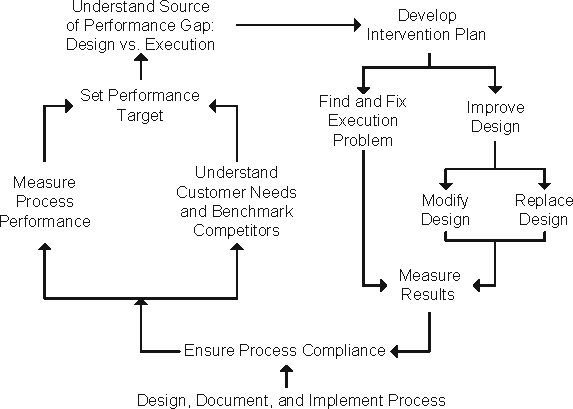
\includegraphics[width=0.8\textwidth]{Images/process_management_cycle.pdf}
\caption[Essentieller Zyklus der Geschäftsprozessmodellierung]{Essentieller Zyklus der Geschäftsprozessmodellierung \citep[S. 5]{Brocke2014}}
\label{process_management_cycle}
\end{figure}
\subsection{Business Process Mapping und Business Process Modeling}\label{subsec:BPMappingModeling}
Die Ermittlung und Visualisierung von Geschäftsprozessen stellt eine Teildisziplin im Management von Geschäftsprozessen dar. Gleichzeitig ist sie der Schlüssel zur Anpassung der Geschäftsprozesse, da ein genaues Verständnis der Abläufe für die Anpassung und Verbesserung unerlässlich sind \cite[vgl.][S. 6]{Jacka2009}. Mit dieser Problemstellung befassen sich sowohl Business Process Mapping als auch Business Process Modeling. Der Unterschied zwischen beiden besteht im wesentlichen in der Zielstellung und der damit verbundenen Abstraktionsebene \cite[vgl.][]{Smartdraw}. Process Mapping zielt im Kern auf die Dokumentation eines bestehenden Prozesses ab, weswegen das Unternehmen auf makroskopischer Sicht analysiert wird. Dabei werden die wesentlichen Funktionen und Rollen bei der Transformation des Inputs zum Output betrachtet. Process Modeling hingegen versucht bestehende Prozesse im Detail zu analysieren, um Engpässe aufzudecken und die Effizienz durch Anpassungen zu steigern \cite[vgl.][]{Appian}. Aus diesem Grund sind die dabei entstehenden Modelle detaillierter. Beide Disziplinen verwenden dabei im Idealfall standardisierte Beschreibungssprachen, wobei sich aus der höheren Detailtiefe beim Process Modeling eine höhere notwendige Komplexität der Beschreibungssprache ergibt. Aufgrund der vielen inhaltlichen und methodischen Überschneidungen der beiden Disziplinen kommt es leider häufig zu Verwechslungen beziehungsweise zur synonymen Verwendung beider Bezeichnungen \cite[vgl.][]{Smartdraw}.

Zu den allgemeinen Vorteilen von Process Mapping zählen die bessere Dokumentation der Prozesse, die Möglichkeit den Prozess grafisch zu visualisieren sowie die komplette Sicht auf die vielen verschiedenen Aspekte eines Prozesses \cite[vgl.][S. 8]{Jacka2009}. Neben diesen offensichtlichen Vorteilen gibt es allerdings noch zahlreiche weitere positive Aspekte, deren Wirkungsweise sich erst auf den zweiten Blick erschließt. Beispielsweise erhöht sich die Transparenz der Unternehmensprozesse, wodurch jeder Prozessteilnehmer seine Rolle im kompletten Kontext besser einschätzen kann. Dadurch wird die Wirkung der eigenen Tätigkeiten wesentlich klarer, was das Stolzgefühl der Mitarbeiter stärkt und so zu einer allgemeinen Steigerung der Mitarbeiterzufriedenheit führt. Zudem kann jeder Teilnehmer wesentlich mehr zur stetigen Verbesserung der Prozesse beitragen, da jedem ein holisitischer Blick auf den Prozess gewährt wird. Ein weiterer positiver Nebeneffekt ist die sich zwangsläufig ergebende Kundenorientierung, da für ein sinnvolles analysieren der Prozesse der Blick auf den für den Kunden generierten Output notwendig ist \cite[vgl.][S. 8-11]{Jacka2009}.

Prinzipiell besitzt auch Process Modeling ähnliche Vorteile, wie die bereits für Process Mapping aufgeführten. Aus der Abstraktionsebene und dem sich daraus ergebenden Detaillierungsgrad ergeben sich jedoch weitere Vorteile. Hierbei ist beispielsweise zu erwähnen, dass die Einarbeitung neuer Mitarbeiter durch die entsprechende Prozessdokumentation leichter fällt und dadurch Zeit eingespart werden kann. Durch die Modellierung der Prozesse entsteht sozusagen ein "`Prozesskatalog"' der auch als zentrales Nachschlagewerk fungieren kann. Zudem erlaubt der Detaillierungsgrad der Prozessmodelle, dass Teilaufgaben automatisiert werden können, was einen großen Vorteil darstellt. Dazu wird eine sogenannten Process Engine verwendet, die für den Nutzer beziehungsweise den Mitarbeiter als Schnittstelle zu genormten Prozessen fungiert. Standardaufgaben, wie beispielsweise das Weiterleiten eines Beurteilungsbogens nach der Prüfung, können dann automatisch durch die \ac{IT} ausgeführt werden \citep[vgl.][S. 2-8]{Freund2014}.

\subsection{BPMN 2.0}\label{subsec:BPMN}
Wie in den vorigen Abschnitten erwähnt wurde, nimmt die Visualisierung von Geschäftsprozessen einen wichtigen Standpunkt ein. \ac{BPMN} wird neben anderen Modellierungssprachen wie YAWL, EPK, Petrinetze, UML speziell im Rahmen des Business Process Modeling verwendet \cite[vgl.][S. 9]{Kossak2014}. Mit der ersten veröffentlichen Version im Jahre 2004 durch die \ac{BPMI} gilt BPMN als einer der jüngeren Vertreter der Prozessmodellierungssprachen. 2005 wurde die \ac{BPMI} durch die \ac{OMG} übernommen, die sich in der IT-Welt bereits durch die Entwicklung und Wartung von UML einen Namen gemacht hat. In der Folge wurde der Standard weiterentwickelt, bis er 2011 in der aktuellsten Version 2.0 verabschiedet werden konnte \citep[vgl.][S. 8f.]{Freund2014}. Die Aufnahme in den ISO 19510:2013 Standard und nicht zuletzt die Pflege der Sprache durch die OMG haben den Stellenwert der BPMN in der Vergangenheit stärken können und ihren Einfluss vergrößert \cite[vgl.][S.10f.]{Kossak2014}. Zudem scheint speziell im Vergleich mit anderen Modellierungssprachen der Fokus und der Blickwinkel der Sprache bei der Modellierung industrieller Prozesse am besten den Forderungen der Unternehmen zu entsprechen \cite[vgl.][S.16]{Kossak2014}. Der Vorteil liegt hier darin, dass BPMN eine angenehme Lösung für den Zielkonflikt zwischen Verständlichkeit für alle Betrachter und notwendiger Komplexität zur Modellierung detaillierter Zusammenhänge darstellt \citep[vgl.][S. 11f.]{Freund2014}.

Obwohl auch BPMN nicht fehlerfrei ist und der Standard teilweise Definitionslücken und Inkonsistenzen aufweist sowie fehlende Standardisierung bei den erstellten Modellen zu Inkompatibilitäten zwischen den verschiedenen Tools führt, erscheint es durchaus wahrscheinlich, dass sich diese Modellierungssprache in naher Zukunft als de facto Standard etablieren wird \cite[vgl.][S.161]{Kossak2014}.

Zur Unterstützung beim Verständnis der folgenden Kapitel folgt ein kurzer Überblick zu den Modellierungselementen und Konzepten von \ac{BPMN} 2.0. Der Standard, der auch die Grundlage für die folgenden Ausführungen bildet, wird von der \ac{OMG} in \citep{OMG2011} definiert.

\subsubsection{Elemente der Modellierung}\label{subsubsec:BPMNElemente}

Mit dem Fokus auf Einfachheit und Nachvollziehbarkeit werden die Elemente in \ac{BPMN} in die folgenden fünf Gruppen unterteilt:
\begin{enumerate}
\item Flussobjekte
\item Verbindende Objekte
\item Artefakte
\item Teilnehmer (Pools und Lanes)
\item Daten
\end{enumerate}
Ihre grafische Darstellung ist in Abbildung \ref{bpmn_basic_elements} zu sehen. Über eine Art visueller Notation in Gruppen ist es möglich, die Klasse oder Funktionalität von Elementen aufgrund ihrer Form einzuschätzen. Beispielsweise werden Ereignisse immer in Form eines Kreises dargestellt, wobei auch die Größendimension der verschiedenen Objekte gleich ist.
\begin{figure}[ht]
\centering
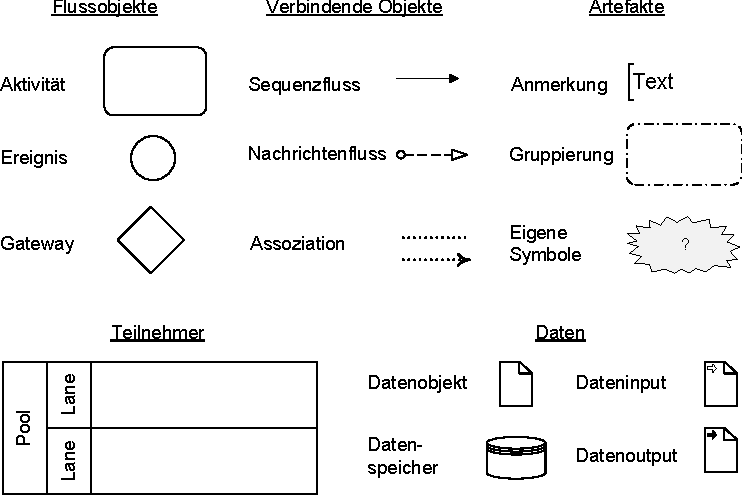
\includegraphics[width=1\textwidth]{Images/bpmn_basic_elements}
\caption[Die Basiselemente der BPMN 2.0]{Die Basiselemente der BPMN 2.0 \citep[S. 23]{Freund2014}}
\label{bpmn_basic_elements}
\end{figure}

Flussobjekte stellen die Kernelemente der Visualisierung dar und beschreiben das Verhalten des Geschäftsprozesses. Dazu unterteilen sich Flussobjekte in Aktivitäten, Ereignisse und Gateways \citep[vgl.][S. 29]{Laliwala2014}. Aktivitäten und Ereignisse erklären sich über ihren Namen sehr gut von allein und stehen somit stellvertretend für durchgeführte Aktionen (Aktivitäten), eintretende Ereignisse oder "`Dinge"', die passieren können. Gateways wiederum stellen bedingte Verzweigungen dar und sind somit essentiell für komplexere Abläufe \citep[vgl.][S. 23]{Freund2014}.

Über den Sequenzfluss wird festgelegt, welche Elemente miteinander verbunden sind  und in welcher Reihenfolge (angezeigt durch die Pfeilrichtung) sie vom Prozess durchlaufen werden. Diese Form des Prozessflusses findet allerdings nur innerhalb eines Pools oder einer Lane statt, weswegen für poolübergreifende Interaktionen Nachrichtenflüsse notwendig sind. Generell werden mit Pools und Lanes verschiedene Rollen, Personen oder andere Entitäten unterschieden und einzelne Elemente durch ihre Position innerhalb einer Lane oder eines Pools den entsprechenden Entitäten zugewiesen. Artefakte sollen zusätzliche Hinweise zum Prozess geben, ohne seine konkrete Ausführung zu verändern. Zur Verbindung von Artefakten mit anderen Objekten werden Assoziationen verwendet. Datenobjekte lassen darauf schließen, welche Daten im Laufe eines Prozesses entstehen oder verwendet werden und lassen sich ebenfalls über Assoziation mit Aktivitäten verknüpfen \citep[vgl.][S. 23f.]{Freund2014}. 
\subsubsection{Diagramm, Prozessmodell und -instanz}\label{subsubsec:BPMNModellInstanz}
Für das eindeutige Verständnis sollten die beiden Begriffe Prozessmodell und Prozessinstanz und der Unterschied zwischen beidem bekannt sein. Ein Prozessmodell beschreibt die modellierte Abbildung der Realität, also eines Prozesses, wovon ein oder mehrere in einem Diagramm enthalten sein können. Von einer Prozessinstanz wird gesprochen, wenn es um eine konkrete Ausführung eines Modells geht. Somit können mehrere Prozessinstanzen vom gleichen Prozessmodell aktiv sein. Man könnte dies auch als einen "`Vorgang"' beschreiben \citep[vgl.][S. 25f.]{Freund2014}.
\subsubsection{Token}\label{subsubsec:BPMNToken}
Das Token ist ein theoretisches Konzept, was bei der Analyse und dem Verständnis eines Prozessmodells hilft. Dabei stellt das Token ein Objekt dar, das in einem Start Event erstellt wird,  das Modell entlang der Fluss- und Verbindungselemente durchläuft und in der Regel durch ein End Event konsumiert wird. Solange ein Token im Prozessmodell "`unterwegs"' ist, bleibt die Instanz aktiv \citep[vgl.][S. 27]{OMG2011}. Gateways besitzen in diesem Zusammenhang eine besondere Bedeutung, da sie abhängig von ihrer Funktion Token vervielfachen oder verringern (konsumieren) können. Wie das Konzept des Tokens bei der Analyse verwendet wird, kann im folgenden Abschnitt bei der Erklärung eines konkreten Beispiels entnommen werden.
\subsubsection{Beispiel}\label{subsubsec:BPMNBeispiel}
Mit Hilfe eines Beispiels soll die Notation der BPMN und das Token-Konzept näher erläutert werden. Aus diesem Grund wurde ein Beispiel aus \citep{OMG2010} gewählt, welches allgemein leicht verständlich ist, aber trotzdem einen guten Querschnitt über die verfügbaren Modellierungselemente der BPMN 2.0 darstellt. Im gewählten Beispiel, das in Abbildung \ref{bpmn_pizza_collaboration} dargestellt wird, wird der Bestell- und Liefervorgang einer Pizza modelliert.
\begin{figure}[ht]
\centering
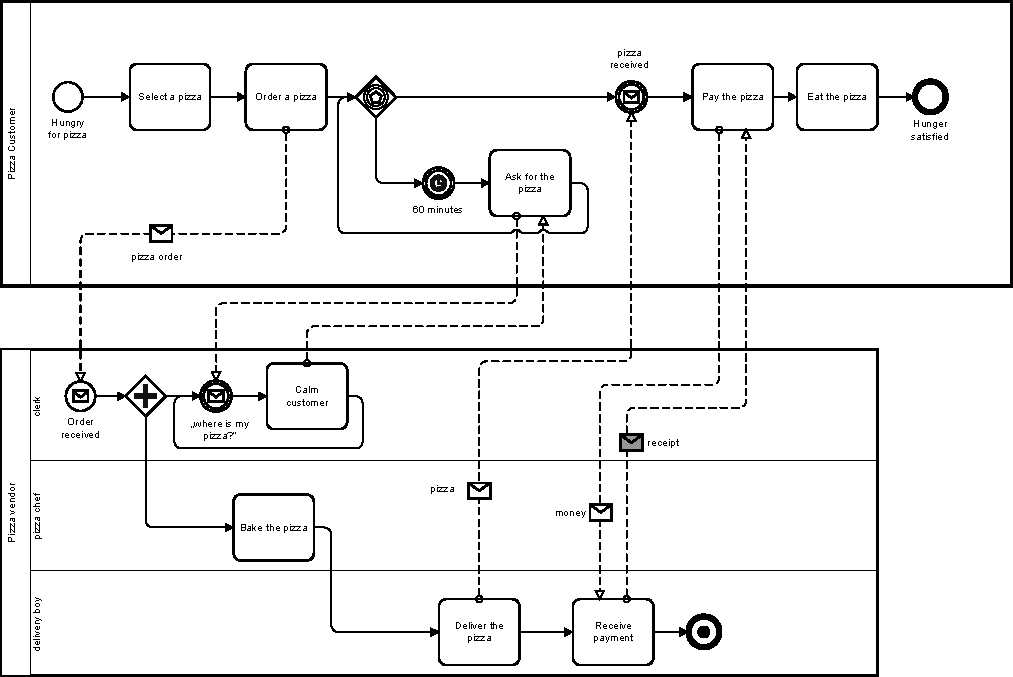
\includegraphics[width=1\textwidth]{Images/pizza_collaboration}
\caption[Bestell- und Liefervorgang einer Pizza]{Bestell- und Liefervorgang einer Pizza \citep[S. 4]{OMG2010}}
\label{bpmn_pizza_collaboration}
\end{figure}

Als erstes fällt auf, dass der gesamte Prozess durch 2 Pools umgesetzt wird. Ein Pool symbolisiert in der BPMN immer eine übergeordnete Instanz, die die darin eingebetteten Lanes steuert. Eine Lane wiederum steht für eine Rolle im Prozess, die entsprechend ihrer Rolle Aufgaben durchführt oder abarbeitet. Diese Denkweise wird von dem Ziel der Automatisierung der Prozesse getrieben, da eine zentrale steuernde Instanz im Kontext eines Prozesses durch eine Process Engine sehr leicht abgelöst werden kann \citep[vgl.][S. 96ff.]{Freund2014}.

Das Startereignis liegt beim Konsumenten der Pizza, der Hunger auf eine Pizza verspürt. An dieser Stelle wird das Token generiert, welches dann zu den nächsten Prozessschritten weiterläuft. Nachdem eine passende Pizza ausgewählt wurde, wird der eigentliche Bestellvorgang ausgelöst. Dazu wird, vermutlich durch einen Anruf oder per Onlinebestellung, eine Nachricht ("`pizza order"') für die Bestellung an den Angestellten des Pizzaverkäufers abgesetzt, was durch den gestrichelten Signalfluss und den Brief angezeigt wird. Anschließend wartet der Kunde auf seine Bestellung. Durch das eventbasierte Gateway wird abhängig vom ersten eingetroffenen Ereignis entweder der Bezahlvorgang eingeleitet (bei Erhalt der Pizza) oder beim Lieferanten nachgefragt, wo die Bestellung bleibt. Das Token verweilt somit im Gateway, bis eines der beiden Ereignisse ausgelöst wird, um dann dem ersten Ereignis zu folgen (XOR-Logik). Für den Bezahlvorgang wird ebenfalls der Austausch von Nachrichten zur Übergabe des Geldes und zum Erhalt der Zahlungsbestätigung verwendet. Anschließend kann der Kunde die Pizza essen und das Token wird im Abschlussevent konsumiert.

Auf der Seite des Pizzaverkäufers signalisiert der Erhalt der Nachricht für die Bestellung den Start. An dieser Stelle wird folglich das Token generiert und läuft in das parallele Gateway. Im parallelen Gateway wird das Token vervielfältigt und es startet auf jeder aus dem Gateway laufenden Prozesslinie ein Token. Eines der Token ist für die Beantwortung der Nachfragen des Kunden zuständig und wartet auf die entsprechende Nachricht, um den Kunden anschließend zu beruhigen. Das zweite Token läuft zum Pizzachef, der die bestellt Pizza bäckt. Danach wird der Prozess beim Botenjungen fortgesetzt, der die Pizza ausliefert und die Bezahlung erhält. Am Ende des Prozesses des Pizzaverkäufers gibt es mit dem Terminierungsereignis noch eine Besonderheit. In diesem Fall reicht ein normales Abschlussereignis nicht aus, da der Prozess ansonsten nie enden würde. Der Grund liegt in dem Zweig, der sich um die Kundennachfragen kümmert. Das Token, das aus dem parallelen Gateway in diese Schleife gestartet ist, kann niemals konsumiert werden, da es selbst nach Auslieferung der Pizza noch auf Nachfragen des Kunden warten würde. Aus diesem Grund wird mit Hilfe des Terminierungsereignisses der gesamte Prozess beendet und alle noch aktiven Token sofort gelöscht.

Nach diesem kurzen Exkurs in die Prozessmodellierung, welcher die Grundlagen für die Methoden und das praktische Vorgehen im Rahmen dieser Arbeit aufgezeigt hat, wird im folgenden Kapitel der rechtliche Rahmen und damit das Hintergrundbild bei der Entwicklung medizinischer Produkte beleuchtet.

\section{Regulatorische Anforderungen für Medizingeräte}\label{sec:RegRequ}
Der Markt für Medizinprodukte gehört zu den stark reglementierten Märkten, in dem Unternehmen speziellen Anforderungen unterliegen. Prinzipiell ist dieses Thema sehr vielschichtig, da die Normen ein recht komplexes Gebilde erstellen, weswegen an dieser Stelle nur eine kurze Zusammenfassung, die für das Verständnis der folgenden Kapitel aber essentiell ist, gegeben werden kann. Im späteren Verlauf dieser Arbeit werden die Anforderungen der Prozesse nach dem Inverkehrbringen aus den gesetzlichen Vorgaben der Europäischen Union abgeleitet und mit dem tatsächlichen aktuellen Prozess verglichen.

Besonders wichtig und interessant ist hierbei die Frage wo die Grenzen dieses Marktes sind und welche Unternehmen und Produkte tatsächlich betroffen sind. Dazu finden sich in der Regel in den Normen und Standards entsprechende Definitionen, die eine Abgrenzung ermöglichen. Folgend ist ein Beispiel der \ac{GHTF} gegeben, welches den Begriff "`medizinisches Gerät (Medical Device)"' erläutert \citep[][S. 6]{GHTF2012}.
\begin{quote}
"`Medical device"' means any instrument, apparatus, implement, machine, appliance, implant, reagent for in vitro use, software, material or other similar or related article, intended by the manufacturer to be used, alone or in combination, for human beings, for one or more of the specific medical purpose(s) of:
\begin{itemize}
\item diagnosis, prevention, monitoring, treatment or alleviation of disease,
\item diagnosis, monitoring, treatment, alleviation of or compensation for an injury,
\item investigation, replacement, modification, or support of the anatomy or of a physiological process,
\item supporting or sustaining life,
\item control of conception,
\item disinfection of medical devices,
\item providing information by means of in vitro examination of specimens derived from the human body;
\end{itemize}
and does not achieve its primary intended action by pharmacological, immunological or metabolic means, in or on the human body, but which may be assisted in its intended function by such means.
\end{quote}

Aus dieser Definition leitet sich für medizinische Geräte eine besondere Verbindung zur Gesundheit des Patienten ab, was einen wesentlichen Unterschied zu anderen Märkten darstellt. Während beispielsweise auf dem Markt für Consumer Electronics die Funktionalität im Fokus des Anwenders und Kunden steht, ist es auf dem Markt für Medizintechnik die Sicherheit des Patienten, die genauso wichtig ist, wie der Kundennutzen beziehungsweise zusammen mit dem Risiko in einem angemessenen Verhältnis stehen muss. Oberstes Anliegen für eine Unternehmung ist jedoch bekanntermaßen in der Regel die Gewinnmaximierung, weswegen hier der Gesetzgeber eine wichtige Rolle übernimmt und die notwendige Sicherheit der Produkte einfordert. Das Ergebnis davon sind Standards und Normen, die vor der Markteinführung eines neuen Produktes erfüllt werden müssen \citep[vgl.][S. 3]{Higson2002}. Als Standard wird eine vereinbarte, wiederholbare Vorgehensweise bezeichnet, die durch ein Dokument festgelegt wird, das durch die Arbeit und Abstimmung eines verantwortlichen Ausschusses erarbeitet wird. Enthalten ist in der Regel eine technische Spezifikation oder andere präzise Kriterien, die als Regel, Richtlinie oder Definition fungieren\citep[vgl.][S. 125-143]{Wong2013}.

Der Einsatz von Normen und Standards in der Medizintechnik ist kein neues Vorgehen, sondern hat sich über die letzten Jahrzehnte etablieren können. Die erste Anforderung zum Einsatz eines Qualitätsmanagementsystems wurde bereits 1976 in den USA eingeführt \citep[vgl.][S. 5]{Higson2002}.
\subsection{Sicherheit medizinischer Geräte}\label{subsec:Safety}
Wie bereits in Kapitel \ref{sec:RegRequ} angesprochen, besitzt die Sicherheit medizinischer Geräte eine besondere Bedeutung. Auch hierfür liefert die \ac{GHTF} eine Definition für eine essentielle Perspektive auf das Thema Sicherheit \citep[][S. 6]{GHTF2012b}.
\begin{quote}
Medical devices should be designed and manufactured in such a way that, when used under the conditions and for the purposes intended and, where applicable, by virtue of the technical knowledge, experience, education or training, and the medical and physical conditions of intended users, they will perform as intended by the manufacturer and not compromise the clinical condition or the safety of patients, or the safety and health of users or, where applicable, other persons, provided that any risks which may be associated with their use constitute acceptable risks when weighed against the benefits to the patient and are compatible with a high level of protection of health and safety.
\end{quote}
Aus dieser Definition geht klar hervor, dass die oberste Pflicht des Herstellers die Sicherstellung der Sicherheit für die Anwender und Patienten ist. Relativiert wird diese Aussage lediglich durch den Zusatz, dass Risiken immer im Verhältnis zum erwarteten Patientennutzen stehen müssen. Ein hohes Risiko für den Patienten ist somit nur akzeptabel, wenn die durchgeführten Aktionen zu einer bedeutenden Verbesserung des Gesundheitszustandes des Patienten führt. Diese Abwägung findet in einem entsprechenden Evaluierungsprozess vor der Markteinführung statt \citep[vgl.][S. 11]{Ramakrishna2015}. 

Absolute Sicherheit kann nicht garantiert werden, da jedes Gerät bis zu einem gewissen Grad ein Risiko in sich trägt und Fehler unter speziellen Umständen auftreten können. Aufgrund unvorhersehbarer Bedingungskonstellationen können Fehler unerwartet und zufällig auftreten, was selbst durch ausgiebige Tests im Vorfeld nicht ausgeschlossen werden kann. Deswegen wird versucht durch Risikobetrachtungen und -analysen die Gerätesicherheit sicherzustellen, indem die vom Gerät ausgehende Bedrohung durch Risikobewertungen abgeschätzt wird. Diese Form der Betrachtung wird auch unter Risikomanagement subsumiert, das sich in der Regel auf die Erfahrung von Experten für Medizintechnik stützt \citep[vgl.][S. 3]{Cheng2003}.

Aber nicht nur der Hersteller medizinischer Geräte allein trägt die Verantwortung für die Sicherheit. Jeder der betroffenen Stakeholder, bestehend aus Hersteller, Regierung, Öffentlichkeit/Patient, Benutzer und Verkäufer, trägt einen Teil zur Gewährleistung der Sicherheit bei. Diese Verantwortung ist in Abbildung \ref{qs_shared_resp} veranschaulicht. Die Rolle des Herstellers ist vermutlich die größte und liegt durch das Design, die Entwicklung und die Produktion des Produktes klar auf der Hand. Die Regierung ist dafür zuständig, dass die in dem jeweiligen Land verfügbaren Geräte sicher und nützlich sind. Der Verkäufer hat als Schnittstelle zwischen Hersteller und Benutzer eine besondere Verantwortung, durch die Überwachung der Konformität zu den regulatorischen Normen und der Bereitstellung des Kundenservice. Der Nutzer des Gerätes wiederum muss sicherstellen, dass er die Funktion des Gerätes erfasst hat und es sicher bedienen kann. Auf den ersten Blick mag es nicht sofort ersichtlich sein, in welcher Weise die Öffentlichkeit und der Patient die Sicherheit beeinflussen können, aber auch der gesellschaftliche Druck auf einen Hersteller zur Erfüllung einer entsprechenden Norm kann am Ende zur Erhöhung der Produktsicherheit beitragen \citep[vgl.][S. 7f.]{Cheng2003}.

TODO: JBI --> vllt. Erwähnung der relevanten Risikonormen?
\begin{figure}[ht]
\centering
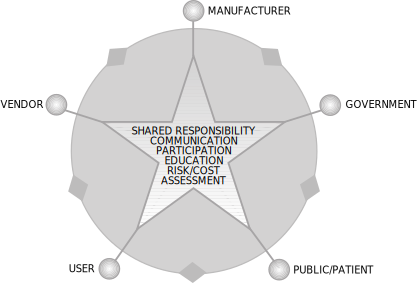
\includegraphics[width=0.8\textwidth]{Images/qs_shared_resp}
\caption[Ideale Bedingungen zur Sicherstellung der Sicherheit medizinischer Geräte]{Ideale Bedingungen zur Sicherstellung der Sicherheit medizinischer Geräte \citep[S. 8]{Cheng2003}}
\label{qs_shared_resp}
\end{figure}
\subsection{Gründe und Bedeutung der Regulierung für Medizinprodukte}\label{subsec:Gruende}
Der Hauptgrund für regulative Normen in der Medizintechnik wurde mit der Verantwortung gegenüber der Patientensicherheit bereits genannt. Dieses Ziel stellt hohe Forderungen an die Hersteller, um die Sicherheit zu gewährleisten. Zur Erfüllung der Anforderungen müssen die Hersteller hohe Aufwände in Kauf nehmen. Interessanterweise hat Regulierung und vor allem Harmonisierung der Normen für die Hersteller aber auch große Vorteile. Durch die Harmonisierung der Normen ist es für die Unternehmen wesentlich einfacher den Marktzugang für ihre Produkte in vielen verschiedenen Ländern zu erreichen. Vor allem im Zeitalter der Globalisierung ist dieser Aspekt sehr wichtig geworden. Würde jeder Gesetzgeber komplett eigene Richtlinien erlassen wäre der Aufwand für die Hersteller immens, wenn sie pro Land und Produkt einen eigenen kompletten Zulassungsprozess durchlaufen müssten.

Mitunter werden Standards eingesetzt, die unter anderem Referenzkriterien schaffen. Erst durch die Festlegung von festen Kennzahlen beziehungsweise messbaren Anforderungen kann die Leistung und Erfüllung von Kriterien transparent werden. Dies ermöglicht danach den Vergleich von Produkten und das Schaffen von Fakten durch die Erfüllung der gestellten Anforderungen. Zudem werden dadurch Informationen bereitgestellt, die die Sicherheit, Verlässlichkeit und Leistung des Produktes oder Services erhöhen. Dies fördert auch für den Nutzer und/oder Patienten die Transparenz über die Gerätecharakteristika. Es kann somit viel besser eingeschätzt werden, welche Eigenschaften ein Produkt hat, und dass für die Bedienung wichtige Anforderungen erfüllt sind, was das Vertrauen bei der Benutzung erhöht. Nebenbei erhält der Konsument die Möglichkeit Produkte eines Herstellers durch die Produkte eines anderen auszutauschen \citep[vgl.][S. 19.]{Cheng2003}.

Zur Prüfung der Konformität mit einem Standard gibt es vier verschiedene Möglichkeiten, die sich jeweils auf verschiedene Abstraktionsebenen beziehen. Die Konformität eines Produktes kann durch direkte Tests sichergestellt werden. Prozesse wiederum können mit Audits geprüft werden, die entweder durch gesonderte Organisationen oder regulatorische Autoritäten durchgeführt werden, die ein entsprechendes Siegel bei Erfüllung vergeben. Ganze Managementsysteme werden auch über Audits geprüft und führen bei Erfüllung der Anforderungen zu Registrierungen in zentralen Karteien (z.B. ISO13485/ISO9001). Die letzte Möglichkeit ist in der Akkreditierung zu sehen, die einer Organisation oder einer Person die formale Erlaubnis erteilen, eine spezielle Aufgabe auszuführen. Ein Beispiel hierfür sind die benannten Stellen in der europäischen Union, die im Medizintechniksektor die Produktkonformitätsprüfung durchführen können, nachdem sie durch eine Autorität des Staates dazu ermächtigt wurden \citep[vgl.][S. 19f]{Cheng2003}.

Prinzipiell kann zwischen verpflichtenden und freiwilligen Standards unterschieden werden. Ein Standard kann durch ein Unternehmen, eine Gesellschaft, Verbände oder ähnliche Institutionen festgelegt werden. Ein Standard kann durch den Gesetzgeber aufgegriffen werden und als verpflichtend eingestuft werden, womit er im jeweiligen Gesetz verankert wird. Die meisten der Standards sind momentan freiwillig, da die Festlegung von Standards als verpflichtende Normen weitreichende Konsequenzen für den globalen Handel hat. Außerdem bedienen die verpflichtenden Vorschriften der Behörden zwar die wesentlichen Sicherheits- und Leistungsprinzipien, dies reicht den Hersteller aber in der Regel nicht aus, da diese noch detailliertere Spezifikationen benötigen. Diesen Detaillierungsgrad können die Behörden aber aufgrund fehlender Ressourcen und Expertise nicht liefern, weswegen freiwillige Standards von den betroffenen Parteien entwickelt werden. Die Vorteile freiwilliger Standards sind vielfältig und liegen beispielsweise darin, dass der Standard von Experten entwickelt wird, die direkten Zugang zu den betroffenen Entitäten besitzen. Zudem wird der weltweite Zugriff auf neue Technologien verbessert, da der Prozess der Harmonisierung der regulatorischen Anforderungen vereinfacht wird. Ein weiterer Vorteil ist darin zu sehen, dass es viel einfacher ist, einen Standard zu aktualisieren, als die Gesetzgebung anzupassen. Die Anpassung des Standards obliegt dem Zusammenschluss von Experten, der ihn entwickelt hat \citep[vgl.][S. 19-22]{Cheng2003}.

Ein Beispiel für eine Organisation, die sich mit der Festlegung von freiwilligen Standards beschäftigt ist das \ac{IMDRF}, das 2012 die \ac{GHTF} abgelöst hat. Das \ac{IMDRF} beschäftigt sich beispielsweise damit fundamentale Definitionen und Frameworks für die Entwicklung medizinischer Geräte zu erarbeiten \citep[vgl.][]{Hall2014}.
\subsection{Überblick über die wichtigsten Standards}\label{subsec:UeberblickStandard}
In Zeiten der Globalisierung wäre es für die Hersteller undenkbar, für jedes Land eine separate Prüfung der Konformität nach nationalem Recht durchzuführen, weswegen von der Industrie Standardisierung gefordert wird \citep[vgl.][S. 6]{Higson2002}. Weltweit gibt es viele verschiedene Organisationen, die sich mit der Normierung beschäftigen und Standards verabschieden. Allerdings ist vorher meist nicht klar, welcher Standard sich durchsetzt und sich im Markt etablieren kann. Zu den wichtigsten Vertretern zählen die ausgearbeiteten Standards der \ac{ISO}. Abbildung \ref{iso_standards} liefert einen Überblick über die wichtigsten Normen für medizinische Geräte.
\begin{figure}[ht]
\centering
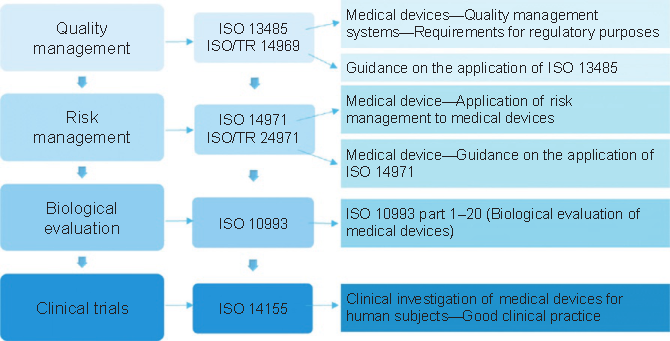
\includegraphics[width=1\textwidth]{Images/iso_standards}
\caption[ISO Standards für medizinische Geräte]{ISO Standards für medizinische Geräte \citep[S. 16]{Ramakrishna2015}}
\label{iso_standards}
\end{figure}
Diese Standards bilden häufig die Grundlage für die Erstellung nationaler Normen. Dabei kann der entsprechende Standard entweder als verpflichtend festgelegt werden oder er wird in eigene Vorschriften des Gesetzgebers überführt, was in Abbildung \ref{iso_standards_adaption} gut erkannt werden kann.
\begin{figure}[ht]
\centering
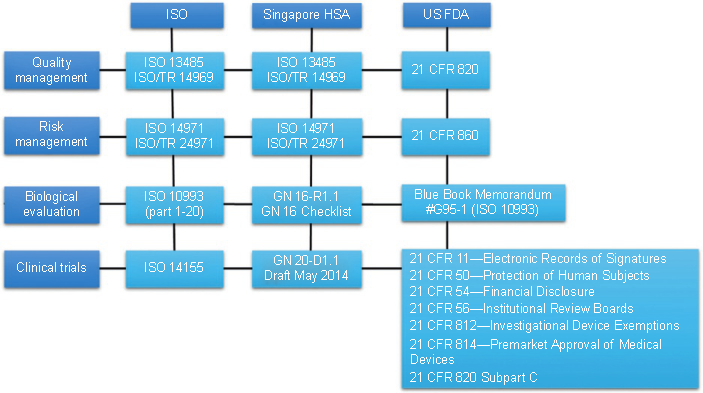
\includegraphics[width=1\textwidth]{Images/iso_standards_adaption}
\caption[Standards und Normen für medizinische Geräte]{Standards und Normen für medizinische Geräte \citep[S. 16]{Ramakrishna2015}}
\label{iso_standards_adaption}
\end{figure}

Zu den wichtigsten nationalen Vertretern mit umfassendem Regulierungssystem zählen \citep[vgl.][S. 14]{Ramakrishna2015}:
\begin{itemize}
\item USA (Food \& Drug Administration(FDA), Center for Devices \& Radiological Health (CDRH))
\item Kanada (Therapeutic Products Directorate)
\item EU (European Commission Directorate, Mitgliedsstaaten)
\item Japan (Ministry of Health, Labour \& Welfare (MHLW), Pharmaceuticals \& Medical Devices Agency (PMDA))
\item Australien (Therapeutic Goods Administration (TGA))
\item China (China Food \& Drug Administration (CFDA))
\item Indien (Drug Controller General of India (DCGI), Central Drugs Standard Control Organization (CDSCO))
\item Singapur (Health Science Authority (HSA))
\end{itemize}

Ein Vorgehen, das sich bei all diesen Vertretern bewährt hat, ist die Einteilung der medizinischen Geräte in verschiedene Risikoklassen, was über den Grad der Kontrollmechanismen und die damit verbundenen Anforderungen an die Hersteller entscheidet (siehe Abbildung \ref{classification_meddev}).
\begin{figure}[ht]
\centering
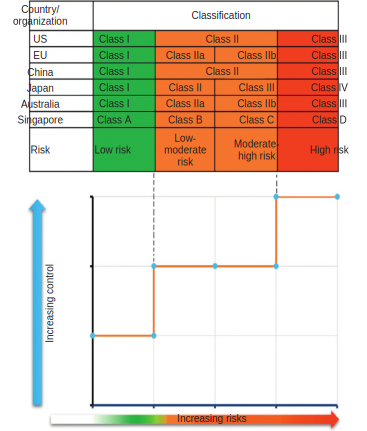
\includegraphics[width=0.7\textwidth]{Images/classification_meddev}
\caption[Einteilung medizinischer Geräte in verschiedene Risikoklassen]{Einteilung medizinischer Geräte in verschiedene Risikoklassen \citep[S. 22]{Ramakrishna2015}}
\label{classification_meddev}
\end{figure}

Diese Arbeit beschäftigt sich im Kern mit den Anforderungen der \ac{MDR} 2017/745, die von der Europäischen Kommission erstellt wurde. Der Fokus liegt somit auf den Regeln in Europa und nicht auf den Statuten der FDA, obwohl diese aktuell aufgrund der Tatsache, dass der Markt in den USA das größte finanzielle Volumen aufweist \citep[vgl.][S. 8]{ITA2016}, weltweit die vermutlich wichtigste Rolle einnimmt.

Die Situation auf dem europäischen Markt ist etwas komplexer als in den USA, da die FDA in den USA als Regierungsunternehmen direkte Befugnisse besitzt. In der EU gibt es neben dem Hersteller insgesamt drei verschiedene Rollen, die für die Regulierung relevant sind. Die Zusammenhänge zwischen europäischer Kommission, staatlicher Behörde, benannter Stelle und Hersteller sind in Abbildung \ref{regulativ_structure_eu} dargestellt. Daraus ist ersichtlich, dass die benannte Stelle für den Hersteller eine sehr wichtige Rolle einnimmt, da sie zum einen den Hersteller überwacht und zum anderen die erstellten Produkte prüft. Die benannten Stellen wiederum werden durch die staatlichen Behörden zugelassen und kontrolliert. Die Europäische Kommission als oberste Instanz legt die zu erfüllenden Normen fest, die von den staatlichen Behörden umgesetzt werden.
\begin{figure}[ht]
\centering
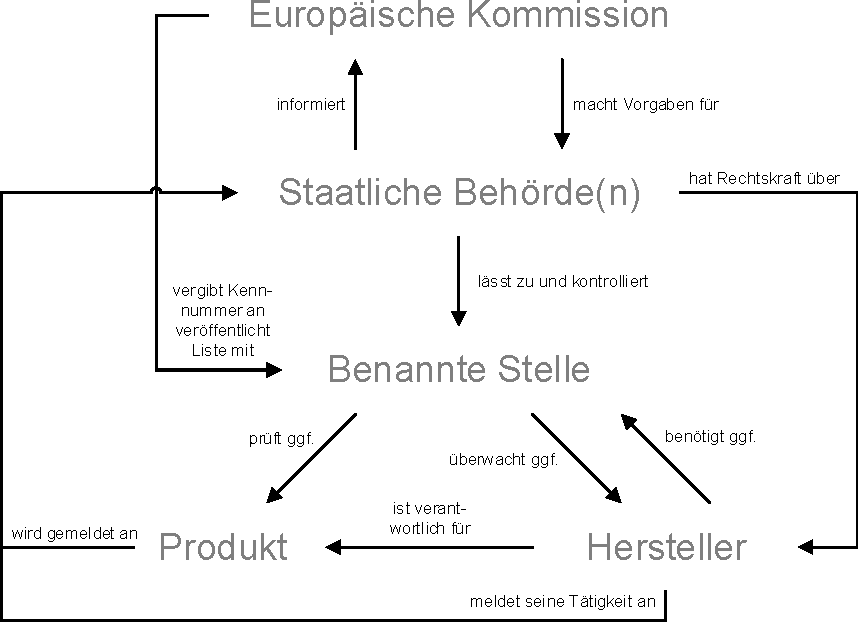
\includegraphics[width=0.7\textwidth]{Images/regulativ_structure_eu}
\caption[Beziehung zwischen Kommission, staatlicher Behörde, benannter Stelle und Hersteller auf dem Medizintechnikmarkt in Europa]{Beziehung zwischen Kommission, staatlicher Behörde, benannter Stelle und Hersteller auf dem Medizintechnikmarkt in Europa \citep[S. 38]{Johner2015}}
\label{regulativ_structure_eu}
\end{figure}

Auf dem Weg zu einem verkaufsfähigen Produkt müssen neben der eigentlichen Entwicklung und Produktion verschiedene Stufen in der europäischen Union durchlaufen werden. Der erste Schritt besteht in der Auswahl der passenden Direktive der europäischen Kommission. Anschließend muss die Risikoklasse bestimmt werden, die die Ausprägung der folgenden Schritte festlegt oder ob sogar Schritte übersprungen werden dürfen. Um die Konformitätsbescheinigung zu erhalten, muss eine Prüfung durch die benannte Stelle erfolgen, die zunächst durch den Hersteller ausgewählt werden muss. Eine Liste der möglichen benannten Stellen wird dazu von der europäischen Kommission zur Verfügung gestellt. Nach erfolgreicher Prüfung erhält der Hersteller die CE-Kennzeichnung, die ihm die Konformität zu den Anforderungen der europäischen Kommission und den erfolgreichen Abschluss der Prüfungen bescheinigt. Mit dieser Bescheinigung kann das Produkt auf dem Markt platziert werden. Während das Produkt im Markt ist, ist der Hersteller zur Meldung von unerwünschten Zwischenfällen und zur ständigen Beobachtung anhand von klinischen Studien verpflichtet \citep[vgl.][S. 32f]{Ramakrishna2015}.
\begin{figure}[ht]
\centering
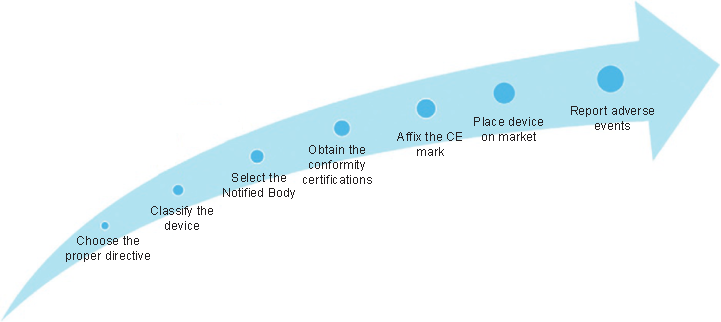
\includegraphics[width=1\textwidth]{Images/route_assure_compliance}
\caption[Route zur Erfüllung regulatorischer Anforderungen für medizinische Geräte in der EU]{Route zur Erfüllung regulatorischer Anforderungen für medizinische Geräte in der EU \citep[S. 33]{Ramakrishna2015}}
\label{route_assure_compliance}
\end{figure}

Der zentrale Rechtsrahmen zur Zulassung medizinischer Geräte in der EU bestand bisher aus den folgenden drei Direktiven, die über die Zeit mehrfach angepasst wurden \citep[vgl.][S. 32]{Ramakrishna2015}:
\begin{itemize}
\item Direktive 90/385/EWG (aktive implantierbare medizinische Geräte)
\item Direktive 93/42/EWG (medizinische Geräte)
\item Direktive 98/79/EG (in vitro diagnostische medizinische Geräte)
\end{itemize}
Durch die neue MDR 2017/745 werden die Direktiven 90/385/EWG und 93/42/EWG ersetzt. Auch die Direktive 98/79/EG wird ersetzt, bekommt mit der IVDR 2017/746 eine eigene Verordnung \citep[vgl.][]{Johner2018}.
\subsection{Auswirkungen auf die Entwicklung und den Produktlebenszyklus}\label{subsec:AuswirkungenAufEntwicklung}
Die vorangegangenen Kapitel haben klargestellt, dass sich Hersteller medizinischer Produkte in einem stark reglementierten Markt bewegen. Die Verantwortung dem Patienten gegenüber und die Anforderungen der Autoritäten schlagen sich in weitreichenden Konsequenzen für den Entwicklungs- und Produktionsprozess nieder. Das Maß der Beeinflussung kann beispielsweise am Fokus der verschiedenen Arbeitsgruppen der GHTF erkannt werden. Auch wenn diese mittlerweile nicht mehr existiert, dient sie immernoch als Vorlage und Querschnitt über die Bemühungen solcher Organisationen. Aus Abbildung \ref{ghtf_focus} ist ersichtlich, dass die Arbeitsgruppen jeweils verschiedene Schwerpunkte setzen (dargestellt als durchgezogene Linie). Über die gestrichelten Linien wird angezeigt, dass der Einfluss jeder Gruppe prinzipiell in jedem Tätigkeitsbereich zu finden ist.
\begin{figure}[ht]
\centering
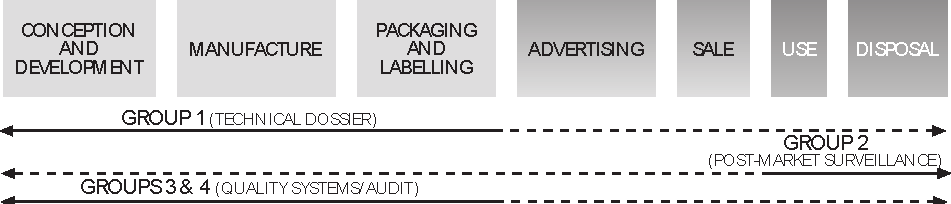
\includegraphics[width=1\textwidth]{Images/ghtf_focus}
\caption[Fokus der verschiedenen Studiengruppen der GHTF]{Fokus der verschiedenen Studiengruppen der GHTF \citep[S. 16]{Cheng2003}}
\label{ghtf_focus}
\end{figure}

Die Anforderungen an den Entwicklungsprozess eines Unternehmens verlangen einen durchgängigen Nachweis der Entwicklungssystematik. In den Normen werden dabei keine konkreten Vorschriften zur Umsetzung gegeben, sondern höchstens unverbindliche Hinweise zur möglichen Umsetzung. Dies stellt die Unternehmen zwar vor große Herausforderungen, lässt ihnen jedoch auch Freiräume bei der Umsetzung. In jeder Hinsicht muss berücksichtigt werden, dass das Ziel entsprechender Normen darin besteht, die Sicherheit der Geräte zu bewerkstelligen und nicht die Gewinnmaximierung der wirtschaftenden Unternehmen durch die Bereitstellung einfacher und günstiger Prozesse in der Entwicklung und Herstellung voranzutreiben. Abhängig von den eigenen individuellen Bedingungen (z.B. Unternehmensgröße, Kultur, spezielle Unternehmensrichtlinien) muss somit jedes Unternehmen nach einer eigenen kostengünstigen und effizienten Lösung suchen \citep[vgl.][S. 103-107]{Johner2015}.

Der Schwerpunkt dieser Arbeit liegt auf der Rückwirkung der nachgelagerten Qualitätsprozesse auf den Entwicklungsbereich, weswegen mit dem Requirements Engineering und dem Product Lifecycle Management folgend die Auswirkungen auf die dafür wichtigsten Schnittstelle im Unternehmen kurz beleuchtet werden sollen.
\subsubsection{Requirements Engineering und Änderungsmanagement}\label{subsec:RQEUndAM}
Generell beschäftigt sich das Requirements Engineering mit dem Erheben und Pflegen der Anforderungen für die Entwicklung eines Produktes. Für das Hauptthema dieser Arbeit soll an dieser Stelle die Bedeutung der Traceability herausgehoben werden, die für die Nachverfolgbarkeit der Anforderungen steht. Die Traceability stellt in vielen Gesetzestexten eine Grundanforderung an die Hersteller dar, da diese zu jeder Zeit über die Gründe wichtiger Entscheidungen berichten können müssen. Für Probleme in Bezug auf Patientensicherheit müssen beispielsweise die einzelnen Schritte zur Behebung von Gefährdungen  nachvollziehbar dokumentiert sein, um die Erfüllung der Sorgfaltspflicht des Herstellers zu belegen. Änderungen von Anforderungen an das Produkt resultieren in der Regel in Änderungen des Produktes. Der Prozess zur Änderung des Produktes, namentlich das Änderungsmanagement, besitzt demzufolge einen besonderen Stellenwert, da durch ihn die Vorgehensweise und Dokumentation bei Produktanpassungen in Folge von Beobachtungen und Feststellungen nach dem Inverkehrbringen festgelegt wird.

"`Unter Traceability versteht man die Nachvollziehbarkeit von Entscheidungen und Abhängigkeiten vom Projektbeginn bis Projektende über alle Informationen und Repräsentationsformen der Darstellung"'\citep[][S. 407]{Rupp2002}. Zu jedem Zeitpunkt einer Entwicklung muss es somit möglich sein, die Quelle für eine entsprechende Anforderung zu ermitteln, was im Rahmen der durch die Autoritäten geforderten Entwicklungssystematik für den Hersteller verpflichtend ist \citep[vgl.][S. 117]{Johner2015}. Dabei wird zwischen horizontaler und vertikaler Traceability unterschieden. Vertikale Traceability betrachtet die Beziehungen zwischen Elementen (z.B. Anforderungen) auf verschiedenen Abstraktionsebenen, womit beispielsweise geklärt werden kann, welcher Test welche Anforderung abdeckt und woher die Anforderung stammt. Horizontale Traceability wiederum stellt die Nachverfolgbarkeit von Elementen vom gleichen Typ und auf gleicher Ebene her und stellt Abhängigkeiten zwischen Anforderungen auf dem gleichen Abstraktionslevel her \citep[vgl.][]{Ebert2014}. Solange ein Produkt noch nicht verkauft wird, sind Informationen wie die Versionshistorie zu jedem Item nur für das Unternehmen selbst interessant. Dies ändert sich jedoch mit der erfolgten Zulassung, denn für Änderungen, die nach der Zulassung erfolgen, muss eine lückenlose Dokumentation erstellt werden. Meist sind solche Änderungen das Ergebnis der "`post-market"' Prozesse, die in Kapitel \ref{sec:PMProzesse} genauer erläutert werden. In der Dokumentation muss beispielsweise erläutert werden, aufgrund welchen Fehlers eine Änderung durchgeführt wurde. Zudem muss die Genehmigung der Änderung anhand der Aufzeichnungen des Entscheidungsgremiums nachvollziehbar sein \citep[vgl.][S. 145f.]{Johner2015}. Dieser ist Prozess allgemein unter dem Namen Änderungswesen (Engineering Change Management) oder Änderungskontrolle bekannt.

Das Änderungswesen ist eine koordinierte Verwaltungsdisziplin, die sich darauf versteht produktbezogene Änderungen zu überwachen. Ziel des Änderungsmanagements ist es demnach Ideen zu sammeln, daraus Lösungsansätze zu erstellen und diese auf ihre technischen und wirtschaftlichen Folgen hin zu untersuchen \citep[vgl.][S. VII]{Prostep2007}. Welch großen Einfluss das Änderungsmanagement für die Entwicklung und Produktion besitzt wird in Abbildung \ref{plm_process_map} deutlich.
\afterpage{
\begin{figure}[p]
\centering
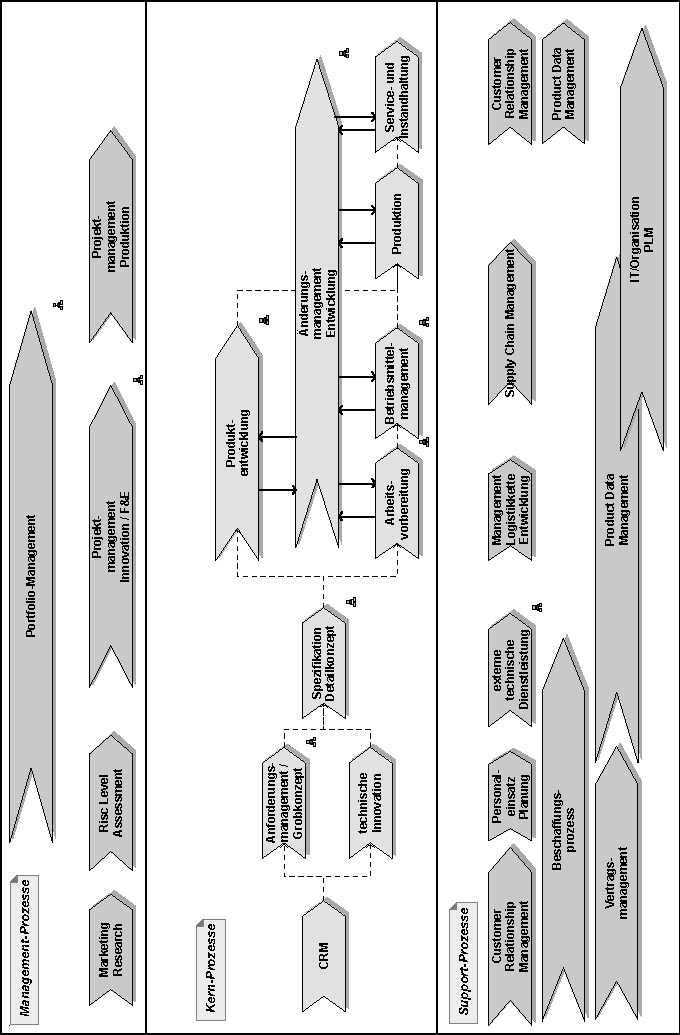
\includegraphics[height=0.9\textheight]{Images/plm_process_map}
\caption[Prozesslandkarte PLM]{Prozesslandkarte PLM \citep[S. 36]{Scheer2006}}
\label{plm_process_map}
\end{figure}
\clearpage
}
In der gesamten Prozesslandkarte besitzt das Änderungsmanagement neben der Produktentwicklung weitere Schnittstellen zur Arbeitsvorbereitung, dem Betriebsmittelmanagement, der Produktion und dem Service und der Instandhaltung. Prinzipiell resultiert die Wichtigkeit des Änderungswesens aus der günstigen Kosten-Nutzen-Konstellation, die sich aus der besseren Erfüllung der Kundenanforderungen durch den direkten Einfluss durch den Nutzer ergibt \citep[vgl.][]{Wu2014}.  Über die Ausprägung des Änderungsprozesses gibt es keinen klaren Konsens, so dass sich verschiedene Formen entwickelt haben, die sich schon allein in der Anzahl der Prozessschritte deutlich unterscheiden. Mindestens besteht der Prozess demnach aus 3 Schritten, aber auch Beispiele mit bis zu 19 Schritten sind bekannt \citep[vgl.][S. 155]{Stark2015}.

Höchste Anforderungen stellt das Änderungsmanagement an die IT, denn die Auswirkungen von veränderten Anforderungen müssen einfach ersichtlich sein und Transparenz sollte möglichst über eine direkte Navigation gegeben sein. Die oberste Anforderung besteht darin auch nach einer Produktänderung konsistente Daten sicherzustellen, um alle historischen Änderungszustände reproduzierbar zu machen \citep[vgl.][S. 85]{Scheer2006}.


\subsubsection{Product Lifecycle Management}
Das \ac{PLM} stellt den Geschäftsprozess dar, der die Produkte eines Hersteller über die erste Produktidee bis zur Abkündigung während ihres gesamten Lebenszyklus begleitet \citep[vgl.][S. 203]{Kale2016}. Somit hilft dieser zentrale Prozess all die Teilprozesse richtig einzuordnen und gibt dem gesamten Produktlebenszyklus auf abstrakter Betrachtungsebene eine gleichbleibende Struktur. Zu den Kernfunktionen zählen zum Beispiel das Produktstrukturmanagement, das Dokumentenmanagement, das Änderungsmanagement oder das Workflowmanagement \citep[vgl.][S. 44]{Saaksvuori2008}. Änderungsvorgänge spielen häufig eine zentrale Rolle in Unternehmen, was auch für die Medizintechnik gilt, da die Pflege von Änderungen eine grundlegende Anforderung für die Hersteller ist \citep[vgl.][S. 175]{Arnold2011}. Der Fokus von \ac{PLM} liegt somit auf Datenmanagement, denn der Kern der PLM Prozesse unterstützt die Aufnahme, Organisation und Wiederverwendung von Wissen über den gesamten Produktlebenszyklus \citep[vgl.][S. 46]{Tayaran2012}.

In Bezug auf Datenmanagement besitzen Informationsflüsse einen speziellen Stellenwert. Häufig sind Informationsflüsse im Anschluss an die Produktauslieferung zum Hersteller nahezu abgeschnitten, wodurch wichtige Informationen aus dem Service und der Wartung verloren gehen und nicht in die Entwicklung und Produktion eingepflegt werden \citep[vgl.][S. 16f.]{Jun2012}. Dieses Vorgehen ist in der Medizintechnik jedoch nicht akzeptabel, da durch die regulativen Anforderungen speziell dieser Informationsfluss in Verbindung mit dem Änderungswesen einen sehr hohen Stellenwert besitzt.
\section{Qualitätsprozesse nach Markteinführung medizinischer Geräte}\label{sec:PMProzesse}
Die Hauptaufgabe eines \ac{QMS} besteht darin die Qualität der durch ein Unternehmen erstellten Produkte sicherzustellen. Um dieses Ziel umsetzen zu können, hat das \ac{QMS} weitreichenden Einfluss auf alle Phasen des Produktlebenszyklus, wozu auch die Aktivitäten nach Markteinführung der Produkte gehören \citep[vgl.][S. 13]{Cheng2003}. Die auf die Markteinführung folgenden Prozesse lassen sich mit den korrigierenden und den präventiven Prozessen in zwei Gruppen unterteilen. Während die korrigierenden Prozesse die Suche nach einer Lösung nach aufgetretenen Problemen oder Vorkommnissen charakterisiert, versuchen die präventive Maßnahmen die Ursache von Problemen bereits vor dem Auftreten zu identifizieren und anschließend zu verhindern \citep[vgl.][S. 338-350]{Abuhav2012}.

Ein funktionsfähiges \ac{QMS} gehört heutzutage in weiten Teilen der Industrie zum Standard. Speziell im Bereich der Medizinprodukte ergeben sich für das QMS jedoch verglichen mit anderen Märkten spezielle Anforderungen, da der Hersteller eine Sorgfaltspflicht dem Patienten gegenüber besitzt und Schäden an Patienten vermieden werden sollen. Während in vielen Branchen der Hauptteil der Arbeit mit dem Markteintritt des Produktes, also mit dem Abschluss der Entwicklung, getan ist, müssen Hersteller für Medizingeräte neben den reinen Supportaufgaben weitere kritische Anforderungen und Pflichten erfüllen, die die Sicherheit der Patienten sicherstellen soll. Der Hauptvorteil für diese Aufgaben das QMS zu bemühen, liegt im präventiven Charakter, der dem modernen Qualitätsansatz innewohnt. Dieser birgt wesentliche Effizienzvorteile gegenüber reaktiven Ansätzen wie beispielsweise Kontrollen am Ende der Fertigungslinie \citep[vgl.][S. 14]{Cheng2003}.

Dieses Vorgehen manifestiert sich durch zahlreiche Normen, die solche Forderungen explizit an das QMS stellen. Dazu gehören unter anderem ISO 13485:2016, ISO 14971:2012, ein von der FDA veröffentlichtes separates Guidance Dokument und die MDR \citep[vgl.][]{Johner2017}. Speziell in Europa war die Gesetzeslage in diesem Kontext jedoch vor der Verabschiedung der MDR nicht zufriedenstellend, da durch fehlende Transparenz und uneindeutige Festlegungen ein viel zu großer Spielraum bestand \citep[vgl.][S. 1]{Chowdhury2014}. Die gestellten Anforderungen erstrecken sich dabei auf das allgemeine Vorgehen, das durch detaillierte Pläne und genaue zeitliche Vorgaben beschrieben wird. Außerdem wird festgelegt, wie mit Zwischenfällen umzugehen ist, da diese mitunter bei regulativen Institutionen bekannt gemacht werden müssen.

Das allgemeine Ziel der daraus resultierenden Prozesse ist es, die Qualität der Produkte zu gewährleisten, indem die notwendigen Daten gesammelt und evaluiert werden. Auf dieser Grundlage kann über die folgenden Aktivitäten und Aktionen entschieden werden. Im folgenden sollen mit \ac{PMS}, \ac{PMCF} und dem Vigilanzsystem drei Komponenten näher vorgestellt werden. Diese drei Komponenten stecken den Beobachtungshorizont der in dieser Arbeit betrachteten betrieblichen Prozesse ab.
\subsection{Post Market Surveillance}\label{subsec:PMS}
Vor der Markteinführung der Produkte müssen Hersteller die Risiken, die von der Benutzung ihrer Produkte ausgehen, minimieren und die Sicherheit der Patienten gewährleisten. Im Rahmen der Zulassung beziehungsweise Konformitätsbewertung wird dies durch die Behörden und die benannten Stellen kontrolliert \citep[vgl.][]{Johner2017}. In der Theorie sollten Produktfehler oder Probleme mit den Produkten somit nahezu ausgeschlossen sein. Die Realität sieht jedoch aufgrund der hohen Komplexität der Anwendungsfälle und der eingesetzten Technik anders aus. Fehler können nie komplett ausgeschlossen werden oder vor der Markteinführung verhindert werden und manche Risiken werden erst im Laufe der Zeit bekannt, wenn die Anwender die Produkte täglich einsetzen. Um diesem Problem zu begegnen wird mit \ac{PMS} analytisch nach Problemen der medizinischen Geräte gesucht, die nicht vor Markteinführung erkannt wurden \citep[vgl.][S. 213]{DeMarco2011}.

Anders als in der vorangegangenen \ac{MDD} wird in \citep[Kapitel 1 Artikel 2 60.]{MDR2017} (MDR) eine genaue Definition für PMS gegeben \citep[vgl.][S. 1]{Pugh2017}: 
\begin{quote}
"`Überwachung nach dem Inverkehrbringen"' bezeichnet alle Tätigkeiten, die Hersteller in Zusammenarbeit mit anderen Wirtschaftsakteuren durchführen, um ein Verfahren zur proaktiven Erhebung und Überprüfung von Erfahrungen, die mit den von ihnen in Verkehr gebrachten, auf dem Markt bereitgestellten oder in Betrieb genommenen Produkten gewonnen werden, einzurichten und auf dem neuesten Stand zu halten, mit dem ein etwaiger Bedarf an unverzüglich zu ergreifenden Korrektur- oder Präventivmaßnahmen festgestellt werden kann. 
\end{quote}

\ac{PMS} (auf deutsch Überwachung nach dem Inverkehrbringen) hat sowohl für den Hersteller als auch den Benutzer große Bedeutung und verfolgt vielfältige Ziele. Zu den Zielen zählt die Risiken des Produktes unter realistischen Situationen systematisch zu identifizieren. Bei der Entwicklung von neuen Geräten werden zwar klinische Tests durchgeführt, diese können allerdings verglichen mit dem späteren Einsatz in der Regel maximal als Stichproben gesehen werde. Zudem sollen Produktfehler und unentdeckt gebliebene Sicherheitsprobleme durch die Analysen aufgedeckt werden \citep[vgl.][]{Johner2017}.

Für den Hersteller ergeben sich tiefe Einsichten in die tatsächlichen Umstände unter denen ihr Produkt agieren muss, was auch kontinuierliche Aktualisierung der Nutzen-Risiko-Bewertung zulässt. Des Weiteren kann die Leistungsfähigkeit der Produkte "`im Feld"' überprüft werden, was für die Produktverbesserung oder Entwicklung von Folgeprodukten eine wichtige Informationsquelle darstellt. Eines der wichtigsten Ziele ist zudem die Einleitung von notwendigen Maßnahmen für Produktrückrufe \citep[vgl.][]{Johner2017}.

Zu den möglichen Datenquellen gehören laut \citep[vgl.][S. 285-288]{Abuhav2012}:
\begin{itemize}
\item Distributoren
\item Kundenbefragungen
\item Service Telefonate
\item Produktbewertungen und Audits
\item Veröffentlichungen in Journalen, Literatur und Fachartikel
\item Forschung und klinische Bewertung
\item Kundenbeschwerden
\item Rückrufe medizinischer Geräte
\end{itemize}

\ac{PMS} stellt zwar zahlreiche Anforderungen an die Hersteller, was aber nicht bedeutet, dass es nicht auch aus Sicht der Hersteller positive Aspekte und Folgen gibt. So wurde bereits angesprochen, dass die detaillierten Informationen, die sich aus der Verwendung der Produkte ergeben, positive Rückwirkungen auf die Produktverbesserung oder die Entwicklung neuer Produkte besitzen. Außerdem kann die Qualität in Folge der Überwachung der Leistung der Produkte verbessert werden. Dies ermöglicht die Qualität zu verbessern, was wiederum zu einer Reduktion der Kosten führen kann \citep[vgl.][S. 2]{Pugh2017}.
\subsection{Post Market Clinical Follow-Up}\label{subsec:PMCF}
\ac{PMCF} (auf deutsch Klinische Nachbeobachtung nach dem Inverkehrbringen) hat das Ziel, die initiale klinische Bewertung zu aktualisieren \citep[vgl.][S. 286]{Abuhav2012}. Auch für die \ac{PMCF} liefert die \ac{MDR} eine detaillierte Definition \citep[Anhang XIV Teil A 5.]{MDR2017}:
\begin{quote}
Die klinische Nachbeobachtung nach dem Inverkehrbringen ist als ein fortlaufender Prozess zur Aktualisierung der klinischen Bewertung gemäß Artikel 61 und Teil A dieses Anhangs zu verstehen und wird im Plan des Herstellers zur Überwachung nach dem Inverkehrbringen behandelt. Bei der klinischen Nachbeobachtung nach dem Inverkehrbringen sammelt und bewertet der Hersteller auf proaktive Weise klinische Daten, die aus der Verwendung eines die CE-Kennzeichnung tragenden, im Rahmen seiner Zweckbestimmung gemäß dem einschlägigen Konformitätsbewertungsverfahren in den Verkehr gebrachten oder in Betrieb genommenen Produkts im oder am menschlichen Körper hervorgehen, um die Sicherheit und die Leistung während der erwarteten Lebensdauer des Produkts zu bestätigen, die fortwährende Vertretbarkeit der ermittelten Risiken zu gewährleisten und auf der Grundlage sachdienlicher Belege neu entstehende Risiken zu erkennen.
\end{quote}

Demnach steht PMCF für das systematische Sammeln von klinischen Daten, um offen gebliebene Fragen, bezogen auf die Sicherheit oder Leistung des Produktes zu klären. Es ist als Untermenge von PMS zu sehen, worauf die MDR explizit hinweist, da PMS alle Arten von bedeutsamen Informationen sammelt. PMS verfolgt zudem das Ziel über notwendige Maßnahmen im Problemfall zu entscheiden und diese einzuleiten, wobei die Erkenntnisse aus den PMCF mit einbezogen werden \citep[vgl.][]{Johner2017}.

Weitere Gründe für die Durchführung von PMCF sind \citep[vgl.][S. 287]{Abuhav2012}:
\begin{itemize}
\item Designänderungen
\item Behandlungsverfahren oder grundsätzliche Verwendung des Gerätes sind neu
\item neue Ansprüche des Herstellers
\item hohes Risiko bei Verwendung des Gerätes
\item Auswertung der Lebenserwartung des Gerätes
\end{itemize}
\subsection{Vigilanzsystem}\label{subsec:Vigilance}
Das Vigilanzsystem übernimmt die Rolle des Marktüberwachungs- und Meldesystems. In ihm werden Festlegungen getroffen, wie die Marktüberwachung gewährleistet wird und wie die Vorkommnisse an die zuständigen Behörden kommuniziert werden. Zur Art und Weise der Kommunikation werden von den Institutionen (beispielsweise die Europäische Union durch die MDR) genaue Forderungen und Vorgaben gestellt \citep[vgl.][]{Johner2017}. Das Ziel ist die Gesundheit und die Sicherheit der Patienten zu schützen, indem Vorfälle bewertet werden und Maßnahmen eingleitet werden, um Wiederholungen zu verhindern. Außerdem wird die Wirksamkeit der Korrektur- und Präventivmaßnahmen bestimmt und Erfahrungen aus der Überwachung gewonnen \citep[vgl.][S. 1]{Pugh2017}.

Auch das Vigilanzsystem stellt allgemein betrachtet eine Untermenge von PMS dar, da vor diesem Hintergrund ebenso die "`post-market"'-Daten ausgewertet werden. Der Fokus des Vigilanzsystems liegt jedoch dabei auf den reaktiven Tätigkeiten, die von den regulativen Autoritäten und dem Gesetzgeber eingefordert werden. Einen großen Stellenwert hat beispielsweise die Einhaltung von genauen Timelines, die abhängig von der Ausprägung des Zwischenfalls verschiedene Anforderungen stellen \citep[vgl.][S. 1]{Pugh2017}.

Jedes Vorkommnis, das mit einem medizinischen Gerät verbunden ist, das in der EU auftritt, muss vom Hersteller genau untersucht werden, um sicherzustellen, ob es an die entsprechende Autorität berichtet werden muss. Ein solcher Bericht stellt eine der möglichen Maßnahmen des Vigilanzsystems dar. Die zweite Form stellt die \ac{FSCA} dar, die für den Hersteller weitreichende Konsequenzen hat. Verbunden mit einem \ac{FSCA} muss auch ein FSCA-Bericht an die regulative Institution gesendet werden \citep[vgl.][S. 1f.]{Loh2017}.
\subsection{Integration in die Entwicklungsprozesse}\label{subsec:IntegrationInDevProzesse}
Die vorgestellten Komponenten für die Sicherstellung der Produktqualität nach dem Marktstart besitzen großen Wert für die Entwicklung. Sie stellen den direkten Rückkanal vom Kunden in das Unternehmen zurück dar und nehmen damit für die Entwicklung und Produktverbesserung eine fundamentale Rolle ein. Die direkte Schnittstelle für die zurückfließenden Informationen stellt das Änderungswesen dar, das in Kapitel \ref{subsec:RQEUndAM} vorgestellt wurde. Vor der Auslösung eines Änderungsvorganges sind jedoch durch die Analyse und Evaluation der Vorkommnisse weitere Unternehmensprozesse vorgeschaltet. Ein Beispiel für einen solchen Prozess ist das Risikomanagement, das die resultierenden Risiken bewertet und durch seine Einschätzung erst weitere Prozesse anstößt.

%===================================================================== Chapter 3
\chapter{Aufnahme des Status Quo bei WOM}\label{chap:AufnahmeStatusQuo}
In diesem Kapitel wird die Modellierung des aktuellen Zustandes beschrieben. Dies stellt den ersten Schritt für eine erfolgreiche Optimierung und Analyse der Prozesse dar, denn erst, wenn alle betroffenen Prozesse erfasst wurden, kann über Veränderungen nachgedacht werden. Zudem erleichtert eine Visualisierung die Diskussion über die einzelnen Elemente und Teilschritte eines Prozesses, da der Ablauf wesentlich leichter erfasst werden kann.
\section{Planung}\label{sec:Planung}
In der Planungsphase werden richtungsweisende Entscheidungen getroffen. Als erstes wird dazu die zu verwendende Modellierungssprache festgelegt. Zukunftsträchtigkeit und Langlebigkeit ist für Unternehmen in solchen Fragen besonders wichtig, da der Mehrwert gering ist, wenn Tools und Methoden verwendet werden, die sich in der Zukunft nicht behaupten können und am Ende schnell wieder substituiert werden. Für die Bearbeitung der gestellten Aufgabe wird deswegen die Notation nach BPMN 2.0 gewählt, da diese einige Vorteile verspricht. Eines der Argumente liegt in der Pflege und Verwaltung durch die \ac{OMG}, die sich auch um den UML-Standard kümmert. Zudem steht BPMN für ein sehr praktikables Verhältnis zwischen Modellierungskomplexität und Intuitivität (siehe \ref{subsec:BPMN}). Dass auch bei WOM erste Überlegungen zur Nutzung von BPMN bei leitenden Prozessverantwortlichen bestehen, sichert die Unterstützung und ermöglicht eventuell die Fortführung der Modelle, sofern die Entscheidung für den ganzheitlichen Einsatz von BPMN für das Unternehmen gefällt werden sollte.

Nachdem die Modellierungssprache festgelegt ist, geht es darum ein passendes Programm auszuwählen, was für die rechnergestützte Modellierung der Prozesse verwendet werden soll. Auch hierfür gab es eine Reihe von Anforderungen, die im Folgenden aufgezählt werden:
\begin{itemize}
\item Support von BPMN Version 2.0
\item Windows 7 kompatibel
\item Freeware, um freie Verwendung und vollen Funktionsumfang für die kommerzielle Nutzung sicherzustellen
\item Standalone Version, die keine Serverinstallation benötigt
\item Regelmäßige Updates und letztes Update innerhalb der letzten zwei Jahre, um sicherzustellen, dass die Software weitgehend fehlerfrei ist und der Standard gut eingehalten wird
\item Exportfunktion für Bilder
\item Unterstützung eines "`interchange formats"', um eventuell Daten später in andere Programme portieren zu können
\end{itemize}
Seitens des Unternehmens werden bis auf die Verwendung eines Freeware-Tools, was auch für die kommerzielle Nutzung komplett freigegeben ist, keine Anforderungen gestellt. Dadurch lässt sich zumindest für die ersten Versuche mit der grafischen Modellierung von Geschäftsprozessen die Anschaffung einer Software umgehen.

Bei dem auszuwählenden Programm soll zudem darauf geachtet werden, dass der Fokus nicht auf der Interaktion mit einem Server liegt. Dies ist gerade bei BPMN sehr naheliegend, da die Automatisierung der Prozesse durch eine Process Engine sehr weit verbreitet ist und zumeist auch einen Kernbestandteil des Geschäftsmodells der Toolhersteller bildet. In diesem Zusammenhang ist oft eine separate Installation eines entsprechenden Dienstes in der Serverarchitektur des Unternehmens notwendig. Dies stellt ein Risiko für die Bearbeitungsfrist dar und sollte demzufolge vermieden werden.

Um bei einer möglichen Fortführung der Arbeiten nicht von vorn beginnen zu müssen, sollte es möglich sein, die entstandenen Daten in ein allgemeingültiges Format zu überführen. Andernfalls müsste das ausgewählte Tool in Zukunft weiter genutzt werden, auch wenn sich die Anforderungen verändern sollten und dadurch ein anderes Programm attraktiver werden würde.

Die Recherche in \citep[][]{Hesse} und in \citep[][]{Naef2012} liefert eine ausführliche Liste mit möglichen Programmen. Nach ausgiebiger Prüfung der einzelnen Vertreter fällt die Wahl auf den Bizagi BPM Modeler \citep[][]{Bizagi}, der alle Anforderungen erfüllt.

\section{Durchführung}\label{sec:durchfuehrung}
Nachdem in der Planungsphase grundlegende Festlegungen getroffen wurden, kann die Analyse der derzeitigen Prozesse begonnen werden. Ein mögliches Vorgehen bei der Modellierung von Geschäftsprozessen wird in \citep[vgl.][S. 13-17]{Jacka2009} beschrieben und besteht aus den folgenden Schritten:
\begin{enumerate}
\item Prozessidentifizierung
\item Datenerfassung
\item Interview und Modellierung
\item Datenanalyse
\item Präsentation
\end{enumerate}
Demzufolge ist die Prozessidentifizierung der Einstieg und besteht daraus, auf abstrakter Ebene die zu modellierenden Prozesse zu benennen. Da dies den Grundstein für die folgende Modellierung legt, ist hierbei besondere Sorgfalt angebracht. Methodisch hilf es in diesem Zusammenhang zunächst die möglichen auslösenden Ereignisse (engl. "`Trigger Events"') zu ermitteln und aus diesen jeweils einen Prozess abzuleiten. Das Ergebnis der Überlegungen ist in Tabelle \ref{tab:trigger_events} abgebildet.
\begin{table}[ht]
\begin{center}
\begin{tabular}{|p{0.6\textwidth}|p{0.3\textwidth}|}
\hline
Trigger Event & Prozessname \\
\hline\hline
Kunde meldet Problem mit Produkt & Kundenrückmeldung \\
\hline
Normative Anforderung zum zyklischen Aktualisierung der klinischen Evaluation & Aktualisierung der klinischen Bewertung\\
\hline
Normative Anforderung den Markt dauerhaft zu beobachten & Marktbeobachtung \\
\hline
Produkt muss zurückgerufen werden & Rückrufaktion, Korrekturmaßnahme im Feld\\
\hline
Fehler im Produkt aufgetreten, weswegen Meldepflicht besteht & Meldesystem\\
\hline
\end{tabular}
\caption[Prozessidentifikation anhand der Trigger Events]{Prozessidentifikation anhand der Trigger Events}
\label{tab:trigger_events}
\end{center}
\end{table}
Demzufolge müssten im Zuge der Modellierung mindestens fünf einzelne Prozesse ermittelt werden können.

Die nächsten beiden Schritte Datenerfassung und Interview beschäftigen sich mit der Problemstellung, die notwendigen Daten zur Prozessmodellierung zu sammeln. Als Hersteller von Medizintechnik ist WOM verpflichtet nach einem Handbuch für das Qualitätsmanagement zu arbeiten (TODO: wo wird das gefordert?). In diesem Handbuch sind die Geschäftsprozesse verteilt über Richtlinien und Verfahrensanweisungen dokumentiert. Da die Auditierungen, die durch die benannte Stelle durchgeführt werden, auf dem QM-Handbuch erfolgen, wird dieses als vorrangige Quelle für die zu modellierenden Prozesse ausgewählt. Dies bedeutet auch, dass etwaige Abweichungen, die sich aus der Befragung der mit den Aufgaben betrauten Mitarbeiter ergeben, ignoriert werden. Mitarbeiterinterviews dienen lediglich als Abgleich und zur Sicherstellung des Verständnisses für die gewonnen Daten. Die Interviews finden mit dem Fachbereichsleiter des Qualitätsmanagement, der die Hauptverantwortung über die analysierten Teile des QM-Handbuches besitzt und mit seinem generellen Überblick die Interpretation der Dokumente bestätigen kann. Zudem wird die Konformität der modellierten Prozesse mit den Dokumenten bezogen auf die normativen Anforderungen der Meldepflicht durch Mitarbeiter der Abteilung Regulatory Affairs verifiziert, da diese in diesem speziellen Teilbereich die entscheidende Instanz bei WOM darstellen.

Ziel ist es die Qualitätsprozesse nach dem Inverkehrbringen der Produkte zu untersuchen, was nur einen Teil des QM-Handbuches darstellt. Um den Aufwand bei der Analyse einzugrenzen, wird zusammen mit dem Fachbereichsleiter des Qualitätsmanagements eine Vorauswahl der relevanten Unterlagen getroffen.

Die Erfassung der Prozesse durch die Analyse des QM-Handbuches stellt sich in der Praxis als schwierig heraus. Dies liegt vor allem an der Struktur des Handbuches, das aus vielen getrennten Verfahrensanweisungen und Richtlinien besteht. Diese scheinen zumindest auf den ersten Blick einen prozessorientierten Grundgedanken zu verfolgen, was sich bei der Analyse allerdings nur teilweise bestätigt. Zwischen den einzelnen Dokumenten, die sich aus Prosatext, Stichpunktanhäufungen und Schaubildern zusammensetzen, bestehen komplexe Zusammenhänge, die sich in zahlreichen Verweisen äußern. Dadurch verteilen sich die einen einzelnen Prozess betreffenden Informationen auf mehrere Dokumente. Ein Überblick über die zu analysierenden Dokumente ist in Abbildung \ref{struktur_dokumente} zu finden, wobei in der Übersicht die Richtlinie 05 für die klinische Validierung nicht vorhanden ist, da diese keine Beziehung zu den restlichen zu betrachtenden Dokumenten aufweist und demzufolge getrennt zu betrachten ist.

\afterpage{
\begin{figure}[p]
\centering
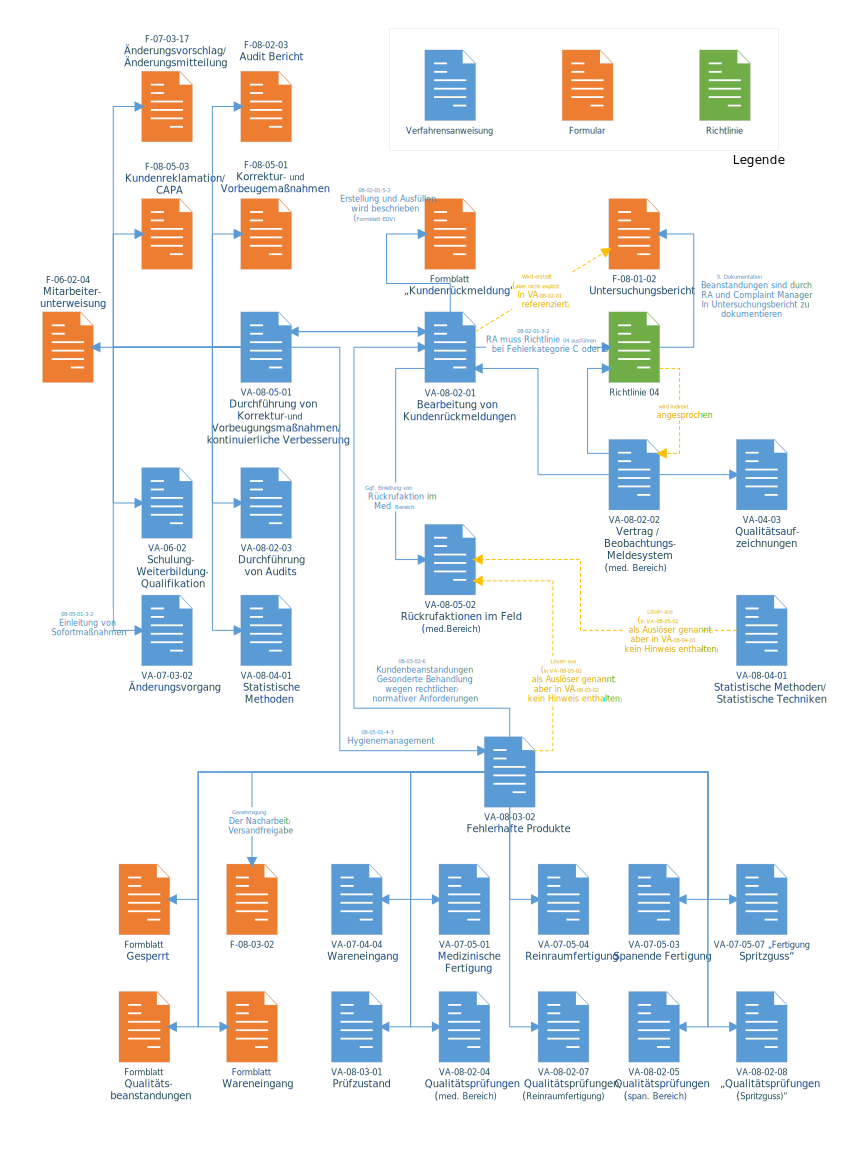
\includegraphics[height=0.9\textheight]{Images/DokumentenstrukturWOM}
\caption[Struktur der Prozessdokumentation (Qualitätsmanagement Handbuch) bei WOM]{Struktur der Prozessdokumentation (Qualitätsmanagement Handbuch) bei WOM}
\label{struktur_dokumente}
\end{figure}
\clearpage
}
Die angesprochene Komplexität bei der Erfassung der Prozesse untermauert den wesentlichen Mehrwert dieser Arbeit für das Unternehmen, da die Unterschiede zwischen dem dokumentierten und dem gelebten Prozess im Nachgang durch die visuelle Darstellung der Prozesse am effektivsten aufgedeckt werden können.

Eine wesentliche Frage, die generell bei der Modellbildung, im speziellen aber bei der Modellierung eines Teilausschnittes, beantwortet werden muss, besteht in der Definition der Modellierungstiefe. Unternehmensprozesse sind in der Regel eng miteinander verzahnt, weswegen enge Grenzen festgelegt werden müssen, um den Aufwand und die Komplexität zu begrenzen. Laut der allgemeinen Systemtheorie besteht ein direkter Zusammenhang zwischen der gewählten Detailtiefe und dem Anwendungshorizont eines Modells \citep[vgl.][S. 49f]{Morecroft2009}. In diesem konkreten Fall bedeutet dies, dass nur die Prozesse komplett modelliert werden, die sich mit den Pflichten des Herstellers nach der Markteinführung beschäftigen. Andere direkt angeschlossene Prozesse werden zur Unterstützung des Verständnisses nur oberflächlich modelliert. Dadurch wird das Zusammenspiel der einzelnen Prozesse und Rollen besser sichtbar, aber der Mehraufwand hält sich in Grenzen. Dieses Vorgehen soll an einem einfachen Beispiel verdeutlicht werden. In den Abbildungen \ref{modellierungstiefe_flach} und \ref{modellierungstiefe_tiefer} ist der gleiche Prozessablauf auf zwei verschiedene Varianten dargestellt. In der Abbildung \ref{modellierungstiefe_flach} wird lediglich der Prozess 1 beschrieben, wobei das Auslösen von Prozess 2 als normaler Schritt in der Abfolge dargestellt ist. In der darauffolgenden Abbildung \ref{modellierungstiefe_tiefer} wird Prozess 2 zwar auch nicht ausgiebig beschrieben, aber durch die grafische Entsprechung, die in der ersten Abbildung komplett fehlt, ist ein wesentlich besserer Überblick gegeben und auf den ersten Blick ersichtlich, dass es sich um zwei Prozesse handelt, die miteinander interagieren.

\begin{figure}[ht]
\centering
\noindent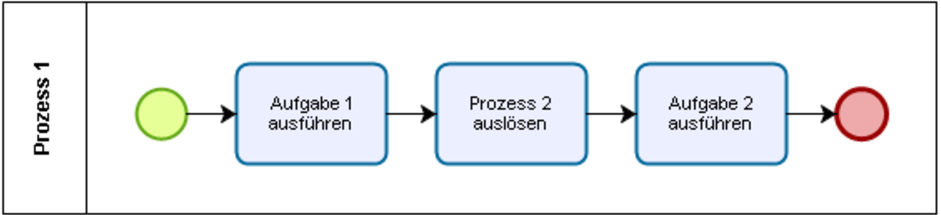
\includegraphics[width=\linewidth,height=\textheight,
keepaspectratio]{Images/modellierungstiefe1}
\caption[Beispiel ohne Darstellung der Interaktion mit anderem Prozess]{Beispiel ohne Darstellung der Interaktion mit anderem Prozess}
\label{modellierungstiefe_flach}
\end{figure}
\begin{figure}[ht]
\centering
\noindent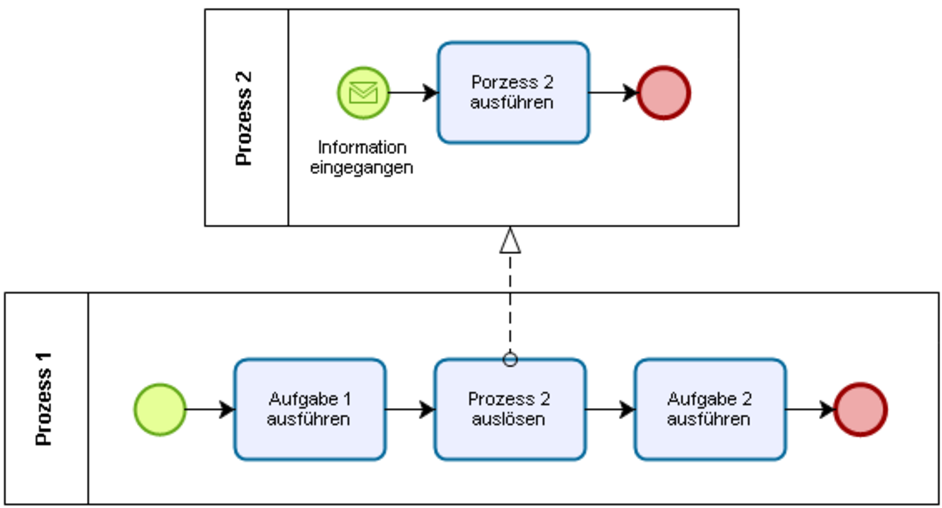
\includegraphics[width=\linewidth,height=\textheight,
keepaspectratio]{Images/modellierungstiefe2}
\caption[Beispiel mit Betonung der Interaktion mit anderem Prozess]{Beispiel mit Betonung der Interaktion mit anderem Prozess}
\label{modellierungstiefe_tiefer}
\end{figure}

Der vorletzte Schritt besteht in der Datenanalyse, der jedoch nicht als klassischer Schritt in einer Reihenfolge zu verstehen ist. Vielmehr findet die Datenanalyse während des gesamten Erhebungsprozesses statt. Bei der Präsentation geht es um den Abschluss und wie das Ergebnis des Prozesmodellierungsprojektes präsentiert wird, beziehungsweise woraus das Ergebnis im Detail besteht. Für das hier zu bearbeitende Projekt wurde bereits im Vorfeld festgelegt, dass ein Modell nach BPMN 2.0 zu erstellen ist. Es wird kein gesonderter Bericht erstellt, der den Prozess genauer analysiert und Verbesserungspotentiale offenlegen soll. Stattdessen soll der Prozess im weiteren Verlauf dieser Arbeit auf die Konformität zur MDR untersucht werden und in diesem Zusammenhang sollen gegebenenfalls Vorschläge erarbeitet werden, wie die Prozesse angepasst werden könnten, um die Anforderungen mit möglichst wenig Aufwand zu erfüllen. Ein zusätzliches Ziel beschäftigt sich wiederum trotzdem mit der Optimierung der Prozesse, wobei allerdings nur die Schnittstelle zum F\&E-Bereich untersucht werden soll.

\section{Vorstellung der Ergebnisse}\label{sec:ergebnisse_modellierung}
In diesem Teilkapitel wird das Ergebnis der Modellbildung präsentiert. Dabei liegt der Fokus auf einem groben Überblick mit zusätzlichen Erklärungen und Hinweisen zu Besonderheiten der BPMN. Aufgrund der Übersichtlichkeit ist es an dieser Stelle leider nicht möglich, sämtliche Ergebnisse aufzuführen, da die entstandenen Modelle zu groß sind. Für einen kompletten Einblick in alle Ergebnisse sei auf den Inhalt der beigelegten Disk verwiesen. Die Modelle liegen dort im HTML-Format vor, so dass sie mit jedem herkömmlichen Browser dargestellt werden können.

Insgesamt konnten die folgenden Prozesse durch die Analyse der Verfahrensanweisungen und Richtlinien bestimmt werden:

\begin{itemize}
\item Bearbeitung Kundenrückmeldung
\item Bestimmung der Fehlerkategorie
\item Meldesystem
\item Rückrufaktion/Korrekturmaßnahme im Feld
\item Änderungsvorgang
\item Statistische Auswertung der Kundenrückmeldungen
\item Statistische Analysen
\item Korrektur- und Vorbeugungsmaßnahmen
\item Aktualisierung der klinischen Bewertung (neue Erkenntnisse)
\item Aktualisierung der klinischen Bewertung (regelmäßig)
\item Fehlerursachenanalyse (Root Cause)
\item Informationen zu Beanstandung einholen
\end{itemize}

Im Modell werden einige Abkürzungen verwendet, die an dieser Stelle zur Absicherung des Verständnisses aufgelöst werden:

\begin{table}[ht]
\begin{center}
\begin{tabular}{|p{0.2\textwidth}|p{0.4\textwidth}|}
\hline
Abkürzung & Auflösung\\
\hline\hline
CEO & Chief Executive Officer\\
\hline
CFO & Chief Financial Officer\\
\hline
CS & Customer Service\\
\hline
DFV & Durchführungsverantwortlicher\\
\hline
F\&E & Forschung und Entwicklung\\
\hline
PJL & Projektleiter\\
\hline
PM & Produktmanagement\\
\hline
QM & Qualitätsmanagement\\
\hline
QMB & Qualitätsmanagementbeauftragter\\
\hline
RA & Regulatory Affairs\\
\hline
UM & Umweltmanagement\\
\hline
\end{tabular}
\caption[Abkürzungen Abteilungen und Rollen]{Abkürzungen Abteilungen und Rollen}
\label{tab:abkuerzungen_abt_rollen}
\end{center}
\end{table}

Der zentralste Prozess im gewählten Themenkomplex wird bei WOM durch die Bearbeitung von Kundenrückmeldungen dargestellt. Dieser Stellenwert kann bereits bei der näheren Betrachtung von Abbildung \ref{struktur_dokumente} erahnt werden, in der sich die Verfahrensanweisung 08-05-01 im Mittelpunkt befindet. Kundenrückmeldungen in verschiedensten Formen sind demnach für das Unternehmen die wichtigste Datenquelle für "`Post-Market-Prozesse"'. Im weiteren Verlauf der Auswertung schließen sich verschiedene Prozesse zur Bearbeitung der Fehler aber auch zur Erfüllung der Meldepflichten an. Für eine bessere Übersicht über die bestehenden Prozesse wird der Prozess der Kundenrückmeldung als Ausgangspunkt für die Modellierung eines Kollaborationsdiagramms verwendet. In diesem wird der Zusammenhang zwischen den Prozessen Kundenrückmeldung bearbeiten, Meldesystem, Rückrufaktion/Korrekturmaßnahme im Feld, Änderungsvorgang und Statistische Auswertung veranschaulicht.

Nachdem die Beanstandungen per Telefon, per Fax oder Brief, durch einen Kundenbesuch oder per Warenrücksendung beim Complaint Manager ankommt, führt dieser die initiale Bearbeitung durch, indem beispielsweise weitere Informationen von der Beanstandungsquelle eingeholt werden. Dieser Teilprozess ist in Abbildung \ref{modell_informationen_einholen} dargestellt.
\begin{figure}[ht]
\centering
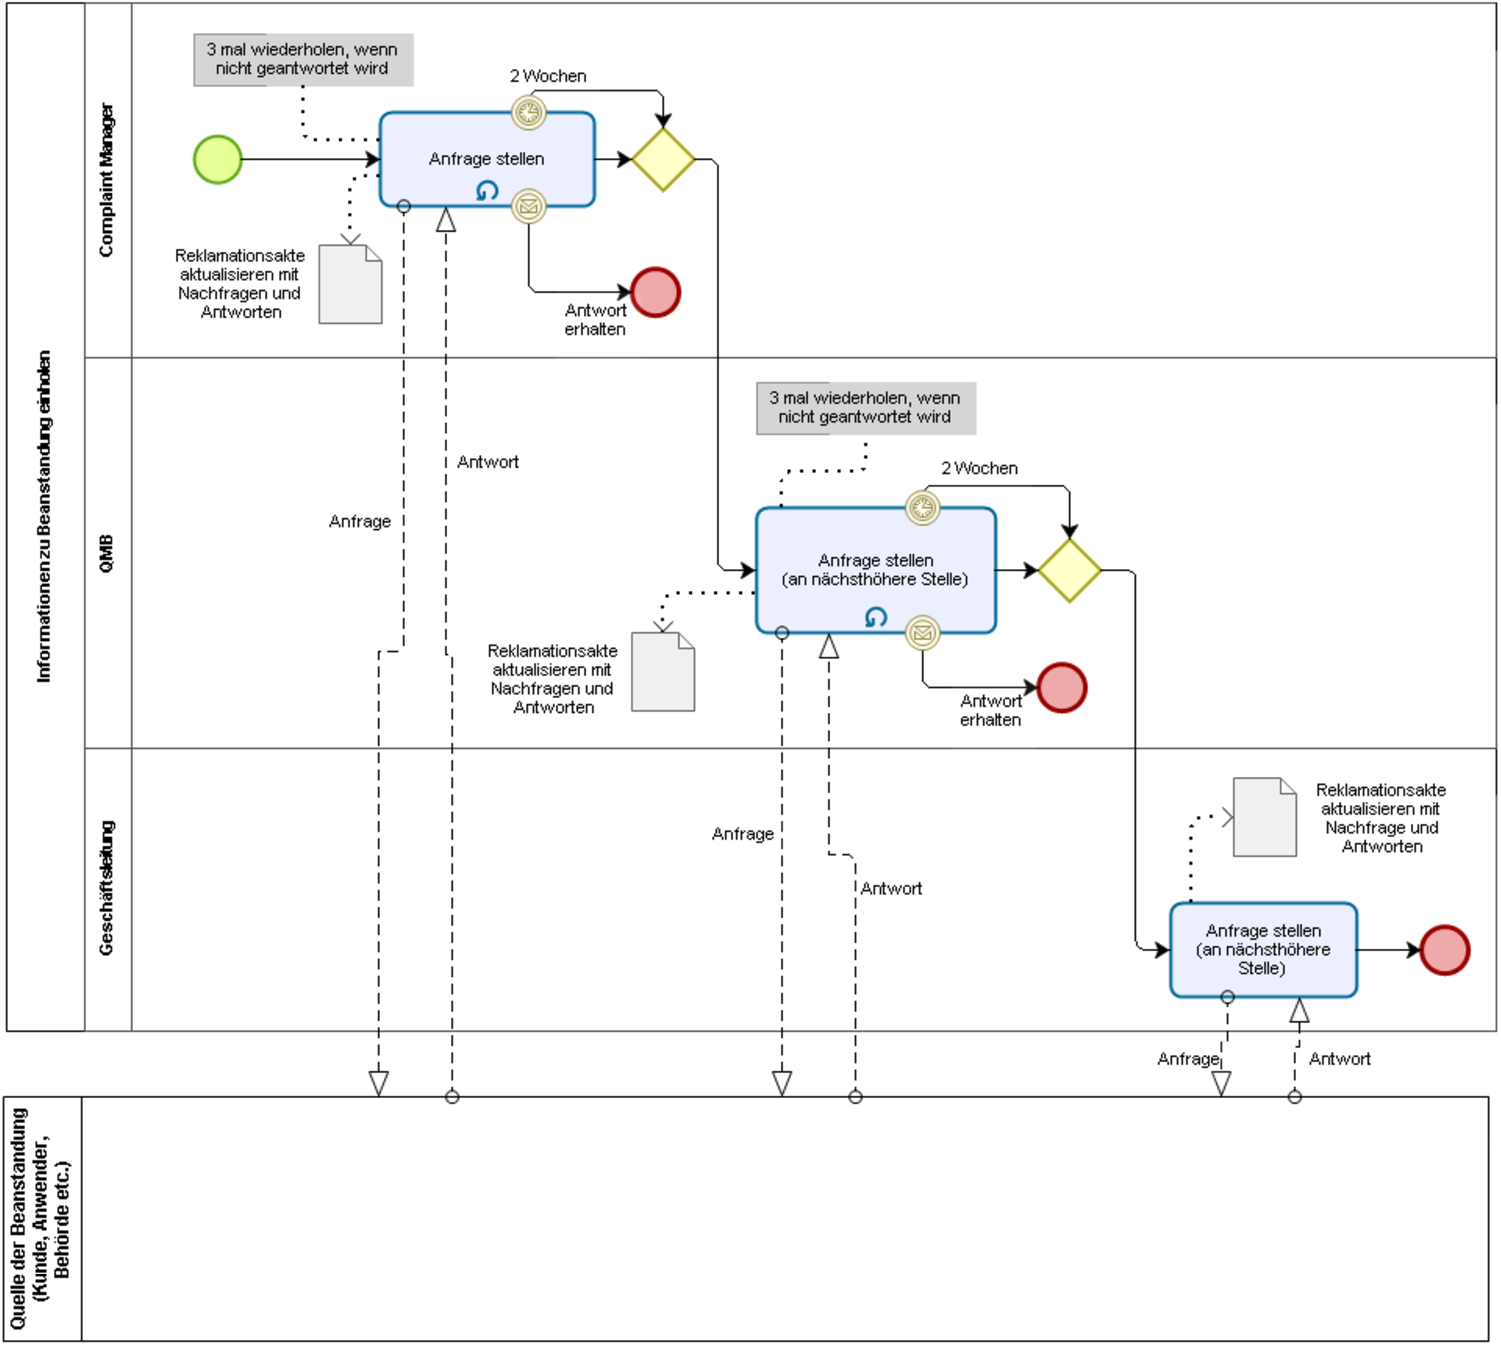
\includegraphics[width=1.0\textwidth]{Images/information_gathering}
\caption[Prozessmodell Informationen zu Beanstandung einholen]{Prozessmodell Informationen zu Beanstandung einholen}
\label{modell_informationen_einholen}
\end{figure}
Aus dem Modell ist zu erkennen, dass es drei Eskalationsebenen gibt, die über die Rollen des Complaint Managers, des QMB und der Geschäftsleitung verteilt sind. Über die Aktivität "`Anfrage stellen"' wird die Interaktion mit dem Kunden durchgeführt. Diese Aktivität wird als Schleife modelliert (zu erkennen an dem kreisförmigen Pfeil), da die Anfrage bis zu drei mal gestellt werden kann. Zudem wird die maximale Dauer, in der eine Antwort eintreffen kann auf zwei Wochen begrenzt, was über das angeheftete Zwischenereignis modelliert wird. Ein zweites unterbrechendes angeheftetes Zwischenereignis wird ausgelöst, wenn eine Antwort erhalten wurde. In beiden Fällen wird die Ausführung der Aktivität unterbrochen. Gibt es innerhalb der Bedingungen keine Rückmeldung vom Kunden, wird die Nachfrage auf die nächste Ebene im Unternehmen gehoben, bis am Ende die Anfrage auf der Ebene der Geschäftsleitung durchgeführt wird.

Aus der Aufgabe "`Anfrage stellen"' wird ein Nachrichtenereignis bis an die Poolgrenze der Quelle für die Beanstandung gesendet. Dies stellt eine Besonderheit der BPMN 2.0 dar, da Nachrichtenflüsse bei nicht vollständigen Modellierungen auch auf die Grenze der Pools gesetzt werden können. Normalerweise müsste ein Nachrichtenfluss mit einem anderen Element (z.B. Ereignis oder Aktivität) verbunden werden, um den tatsächlichen Informationsaustausch aufzuzeigen. Dies ist allerdings wie hier im Beispiel nicht immer möglich, da die internen Prozesse beim Kunden beispielsweise nicht bekannt sind. Über diese Freiheit lassen sich trotz fehlendem Wissen die Interaktionen zwischen den verschiedenen Prozessteilnehmern und Prozessen verdeutlichen.

Nachdem durch den Complaint Manager ein \ac{DFV} benannt wurde, wird mit der Bearbeitung des Fehlers, genauer gesagt mit der Identifikation, fortgefahren. Bereits so früh im Prozess wird die Bedeutung der Meldepflicht offensichtlich, da hier die erste Interaktion mit dem Prozess "`Meldesystem"' stattfindet. Die Interaktion liegt in dem Sinne vor, dass im Rahmen der Bearbeitung der Beanstandung Informationen gewonnen werden, die abhängig von der ermittelten Fehlerkategorie für den Prozess der Meldepflicht sofort zur Verfügung gestellt werden müssen. Schnelles handeln ist besonders wichtig, da durch die normativen Institutionen teilweise sehr enge Zeitfenster für Meldungen eingeräumt werden. So muss beispielsweise der FDA-5-Day Report innerhalb von fünf Tagen ausgelöst werden. Um diese Anforderung durch die Prozesse bedienen zu können, gibt es mehrere Prozessschritte bei der Bearbeitung von Kundenrückmeldungen, wo die Informationen synchronisiert werden. 

Durch die Mitarbeiter der Abteilung RA werden die Meldepflichten ausgehend von der ermittelten Fehlerkategorie bedient. Das aktuelle Modell konzentriert sich gerade bei den Meldepflichten auf den europäischen Raum, da im folgenden Kapitel die Konformität zur neuen europäischen Verordnung MDR untersucht wird. Zusätzlich wird der Prozess für die FDA dargestellt, da die meisten Vorgaben bei WOM auf den FDA-Anforderungen beruhen. Im Detail wird Schritt für Schritt beschrieben, wie mit den Beanstandungen verfahren werden muss. Für den europäischen Raum geht es bis hin zur möglichen Koordination und Durchführung von Korrekturmaßnahmen. Für die FDA besteht wiederum auch nach dem Absenden des Berichtes die Pflicht, weitere Informationen zu sammeln und in einem jährlichen Bericht bei der Behörde den Informationsstand zu aktualisieren. Am Ende steht für beide Vorgehensweisen die Dokumentation der Beanstandung in einem dafür ausgewiesenen Formular.

Parallel läuft die interne Bearbeitung der Beanstandung weiter, indem die Fehlerart bestimmt und im Formblatt EDV eingetragen wird. Anschließend findet eine genaue Ursachenanalyse statt. Dieser Prozess ist nicht trivial, da hierfür die Unterstützung mehrerer Fachbereich hinzugezogen werden kann. Da die Bedeutung dieses Teilprozesses für den Prozess der Bearbeitung einer Kundenrückmeldung vergleichsweise gering ist und die zusätzlichen Rollen im Kollaborationsdiagramm die Übersichtlichkeit verringern würden, wird er in einen eigenen Unterprozess ausgelagert. Hierfür bietet BPMN 2.0 im Wesentlichen zwei verschiedene Varianten an. Die einfachste Form ist der eingebettete Sub-Process. Dieser hat die Aufgabe die Übersichtlichkeit zu erhalten, indem mehrere Aktivitäten und Symbole in einem Symbol geclustert werden. Komplexe Abläufe über mehrere Rollen können dadurch allerdings nicht abgebildet werden. Dazu wird die Call-Activity verwendet, die für einen wiederverwendbaren Teilprozess steht. Dies ermöglicht den Einsatz von Pools und Lanes im Subprozess und lässt verschiedene Startevents zu. Die beiden Symbole sind sich sehr ähnlich, werden durch ein "`+"'-Zeichen signalisiert und unterscheiden sich lediglich in der Dicke des Rahmens des Prozesssymbols \citep[vgl.][S. 173-188]{OMG2011}. Beide Arten werden im hier beschriebenen Modell verwendet. Um den visuellen Unterschied deutlich zu machen, sind in Abbildung \ref{call_activity} die Verwendung einer Call-Actitivty und in Abbildung \ref{sub_process} ein Sub-Process gegenübergestellt.
\begin{figure}[ht]
\centering
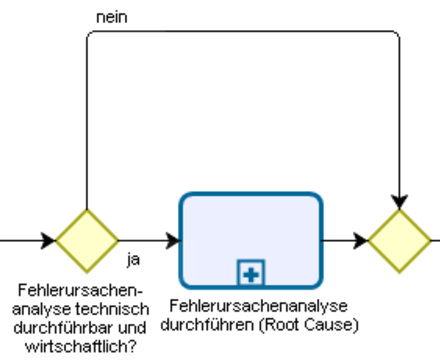
\includegraphics[width=0.5\textwidth]{Images/sub_process_call}
\caption[Anwendung einer Call Activity]{Anwendung einer Call-Activity}
\label{call_activity}
\end{figure}
\begin{figure}[ht]
\centering
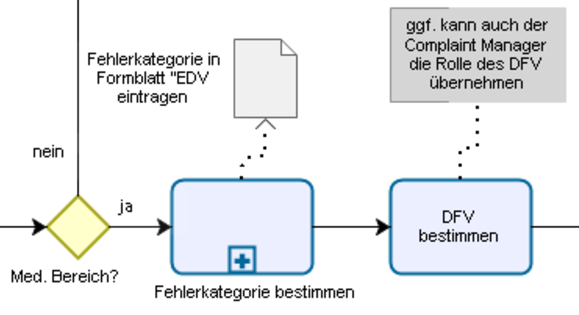
\includegraphics[width=0.5\textwidth]{Images/sub_process}
\caption[Anwendung eines Sub-Processes]{Anwendung eines Sub-Processes}
\label{sub_process}
\end{figure}

Anschließend geht es darum Maßnahmen festzulegen, um das Problem zu beheben. Diese Aufgabe wird parallel von drei Rollen im Prozess ausgeführt. Da sich eine Aufgabe nicht über eine Lane-Grenze hinweg erstrecken kann, aber trotzdem signalisiert werden soll, dass die drei Parteien diese Aufgabe gemeinsam lösen, wird eine Gruppierung mit einem gestrichelten Kasten vorgenommen, der die gleiche Aufgabe auf den verschiedenen Lanes umschließt (siehe Abbildung \ref{shared_task}). 
\begin{figure}[ht]
\centering
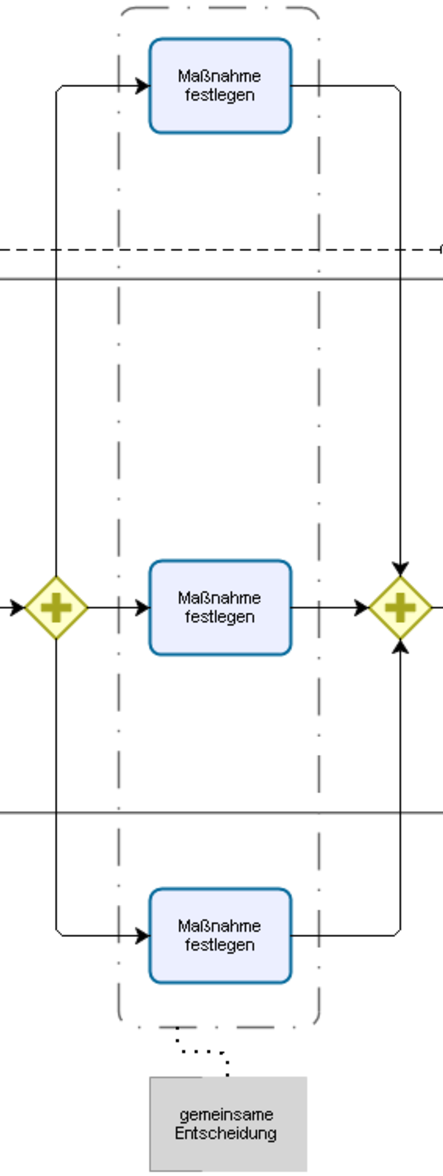
\includegraphics[width=0.3\textwidth]{Images/shared_task}
\caption[Gruppierung von Aufgaben]{Gruppierung von Aufgaben}
\label{shared_task}
\end{figure}

Nachdem die Maßnahmen festgelegt wurden, sollten diese durchgeführt werden. An dieser Stelle wird eine weitere bemerkenswerte Modellierungsmöglichkeit der BPMN eingesetzt. Die möglichen festgelegten Maßnahmen sind sehr vielfältig, weswegen es schwer fällt beziehungsweise es nicht sinnvoll erscheint alle möglichen Konstellationen exakt zu modellieren. BPMN bietet für solche Fälle die Ad-Hoc-Sub-Prozesse an, deren syntaktische Anforderungen wesentlich freier sind, als die des normalen Prozessflusses. Zu erkennen ist diese Form der gekapselten Prozesse an der Tilde im mittleren unteren Bereich des Kastens. Durch die ausführende Instanz kann in der gewählten Konstellation in Abbildung \ref{ad_hoc_process} frei entschieden werden, welche der Teilaufgaben ausgeführt werden und in welcher Reihenfolge \citep[vgl.][S. 180]{OMG2011} \citep[vgl.][S. 431]{OMG2011}. 
\begin{figure}[ht]
\centering
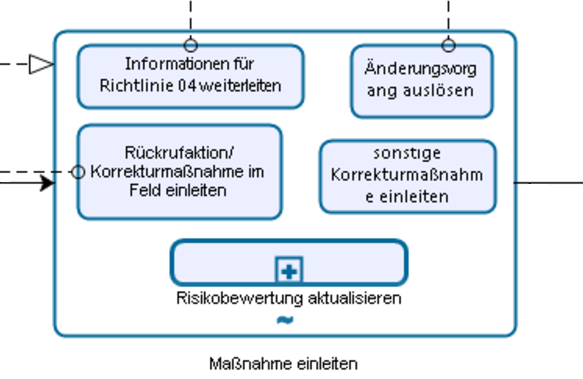
\includegraphics[width=0.5\textwidth]{Images/ad_hoc_process}
\caption[Ad-Hoc-Prozess zur Einleitung von Maßnahmen]{Ad-Hoc-Prozess zur Einleitung von Maßnahmen}
\label{ad_hoc_process}
\end{figure}
Zu den möglichen Maßnahmen gehören dem Meldesystem (Richtlinie 04) neue gewonnene Informationen zukommen zu lassen, einen Änderungsvorgang auszulösen, eine Rückrufaktion/Korrekturmaßnahme im Feld einzuleiten, die Risikobewertung zu aktualisieren oder sonstige Korrekturmaßnahmen einzuleiten. Bis auf den Sammelbegriff für sonstige Korrekturmaßnahmen steht jede Möglichkeit für die Interaktion mit einem anderen Unternehmensprozess. Die Aktualisierung der Risikobewertung wird als wiederverwendbare Call-Activity modelliert, wobei der tatsächliche Prozess aufgrund der gewählten Modellierungstiefe nicht beschrieben wird. Das gleiche Vorgehen wird für den Änderungsvorgang gewählt, der aber aufgrund seiner Allgemeingültigkeit und der hohen Bedeutung für das Unternehmen zumindest als separater Prozess vorgesehen wird. Dadurch findet an dieser Stelle ein Nachrichtenfluss zu dem entsprechenden Prozess statt.

Die vermutlich schwerwiegendste Folge aus der Verarbeitung einer Kundenbeanstandung besteht in einer Rückrufaktion beziehungsweise einer Korrekturmaßnahme im Feld. Da dieser Prozess essentiell für das Vorgehen eines Herstellers für Medizinprodukte bei Fehlern nach der Markteinführung ist, wird er durch eine eigene Verfahrensanweisung und auch im hier vorgestellten Modell in einem separaten Prozess beschrieben. Ein Rückruf kann neben einer Kundenbeanstandung aber auch durch eine Fehlerhäufung, die durch den Einsatz statistischer Methoden erkannt wird, oder durch die Analyse fehlerhafter Produkte in der Produktion ausgelöst werden. Das Thema der statistischen Auswertung spielt im späteren Verlauf der Prozessbeschreibung nochmals eine Rolle und wird an dieser Stelle genauer beleuchtet. 

Nachdem der Prozess zum Produktrückruf durch eines der beschriebenen Ereignisse initialisiert wurde, gilt es zunächst das Risiko einzuschätzen. Diese Vorgehensweise ist fest im Ablauf eines Produktrückrufs verankert, um sicherzustellen, dass die Notwendigkeit tatsächlich gegeben ist. Dazu wird eine Besprechung, bei dem jeweils ein Vertreter aus der Abteilung RA, PM und der QMB anwesend sein müssen, zur Einschätzung des Risikos vom Projektleiter einberufen. Für die Dokumentation der Ergebnisse ist ebenso der Projektleiter zuständig. Die graphische Entsprechung für diesen ersten Teil des Prozesses ist in Abbildung \ref{capa_risk_analysis} zu sehen, wo nochmals die Zusammenarbeit der verschiedenen Rollen durch die Gruppierung aufgezeigt wird.
\begin{figure}[ht]
\centering
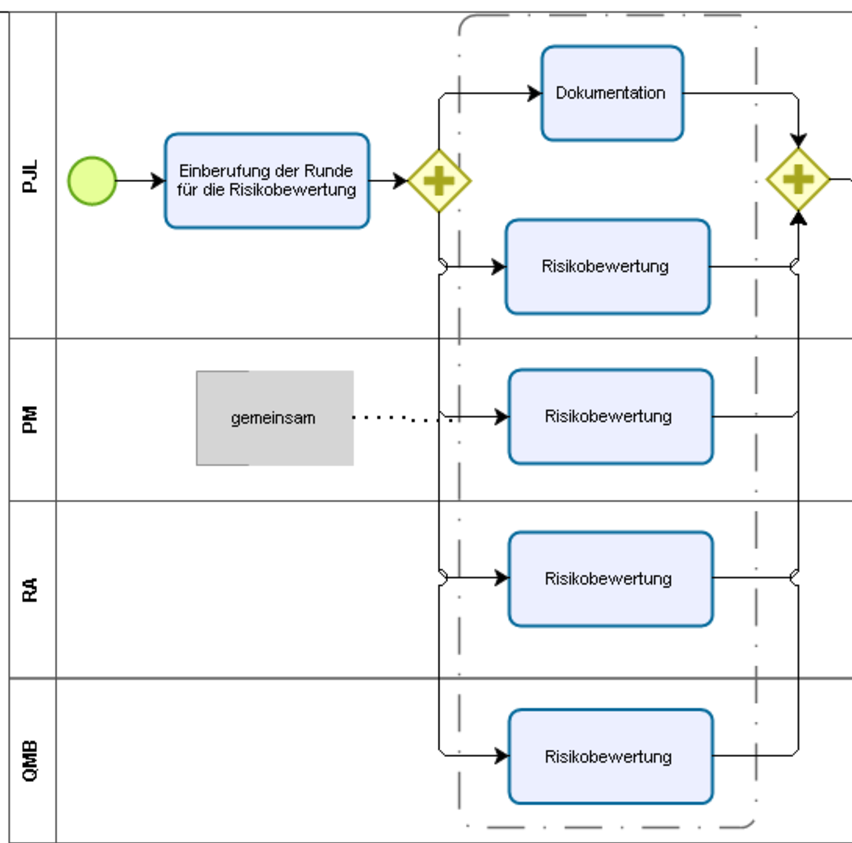
\includegraphics[width=0.6\textwidth]{Images/capa_risk_analysis}
\caption[Risikoanalyse im Rahmen des Produktrückruf-Prozesses]{Risikoanalyse im Rahmen des Produktrückruf-Prozesses}
\label{capa_risk_analysis}
\end{figure}
Die Verletzung gesetzlicher Vorgaben entscheidet am Ende über die Durchführung der Korrekturmaßnahme im Feld. Durch eine entsprechende Verletzung wäre das Unternehmen zu einem Rückruf gesetzlich verpflichtet, weswegen sich die Prüfung dieses Sachverhaltes durch einen Mitarbeiter der Abteilung RA, dem QMB und dem Sicherheitsbeauftragten für den medizinischen Bereich an die Risikobewertung anschließt. Liegt nach dieser Prüfung die gesetzliche Pflicht für eine entsprechende Feldaktion vor, werden durch die gleichen Verantwortlichen die Behörden informiert und die formellen Anforderungen der Rückrufaktion werden abgewickelt.

Neben der Erfüllung der gesetzlichen Forderungen kann sich das Unternehmen auch zu einem freiwilligen Rückruf entscheiden, worüber durch den QMB, den Vertriebsleiter, den CFO und den CEO entschieden wird. Bei der Entscheidungsfindung unterstützen die Bereiche RA, PM und der PJL.

Unabhängig davon, ob der Rückruf freiwillig oder gesetzlich vorgeschrieben ist, wird im Folgenden eine Liste der Kunden und der betroffenen Geräteseriennummern durch den QMB und einen Mitarbeiter der Abteilung PM erstellt. Diese dient als Grundlage für die Absprache zur Durchführung der Aktion mit dem Kunden, die durch den Vertriebsleiter durchgeführt wird. Über die dabei festgelegten Schritte wird der QMB und die Complaint Stelle vom Vertriebsleiter informiert. Die operative Durchführung der firmeninternen Abläufe erfolgt durch den QMB und die Complaint Stelle. Am Ende verbleibt die Erstellung eines Abschlussberichtes durch das PM und den Vertriebsleiter.

Zurück beim Prozess zur Bearbeitung von Kundenrückmeldungen steht nach der Einleitung von Maßnahmen die Dokumentation, Archivierung und Interaktion mit dem Kunden bezogen auf die konkrete Beanstandung aus. Somit wird ein Prüfbericht durch den DFV verfasst, der durch den Complaint Manager beim Vorliegen von Fehlerkategorie C oder D als Grundlage für einen Untersuchungsbericht dient. Der Kunde wird im Rahmen einer Stellungnahme, die durch den Complaint Manager verfasst wird, über die Informationslage informiert. Der Prüfbericht wird zudem zur statistischen Auswertung weitergeleitet.

Die statistische Auswertung besteht aus mehreren parallel voneinander ablaufenden Prozessen. Die Auswertung der Kundenrückmeldungen stellt somit nur einen Ausschnitt der durchgeführten Tätigkeiten dar und wird durch Zusammenarbeit des Complaint Managers und QM erstellt, um eine Datenbasis für das Erkennen von Trends aufzubauen und als Input für das jährliche Management Review zu dienen. Neben diesem Prozess gibt es in den Fachabteilungen Produktion und Materialwirtschaft, Vertrieb und Marketing, QM und UM zahlreiche überwiegend periodisch stattfindende Analysen, die wichtige Entscheidungsgrundlagen für andere Unternehmensprozesse zur Verfügung stellen.

Um den Prozess der Bearbeitung der Kundenrückmeldung abschließen zu können, muss die Wirksamkeit der gewählten Maßnahmen geprüft werden. Dazu wird durch den Complaint Manager der Zeitpunkt für die Wirksamkeitsprüfung festgelegt. Ist das festgelegte Zeitfenster verstrichen, wird durch den Complaint Manager und das Qualitätsmanagement unter Berücksichtigung der statistischen Daten die Wirksamkeit geprüft. Eine Maßnahme wird dabei als wirksam eingestuft, wenn in der Folge keine weiteren Beanstandungen erfasst werden. Die letzten beiden Schritte bestehen aus dem Prüfen der Dokumentation durch den QM-Bereich und eine finale Prüfung der Reklamation durch den QMB.

Eingangs wurde erwähnt, dass der Prozess für die Bearbeitung von Kundenrückmeldungen für WOM eine sehr hohe Priorität besitzt und eine zentrale Stellung bei der Marktbeobachtung nach dem Inverkehrbringen der Produkte einnimmt. Neben diesem gibt es mit dem Prozess für Korrektur- und Vorbeugemaßnahmen und der Aktualisierung der klinischen Bewertung aufgrund neuer Erkenntnisse oder in regelmäßigen Intervallen weitere Prozesse, die berücksichtigt werden müssen.

Bei den Korrektur- und Vorbeugungsmaßnahmen geht es um einen allgemeingültigen Prozess, der bei der Feststellung einer tatsächlichen (auch potentiellen) Abweichung initiiert wird. Aufgrund seiner Allgemeingültigkeit ist er durch die entsprechende Verfahrensanweisung nur sehr grob umrissen, da die Abweichungen und die daraus abzuleitenden Maßnahmen sehr vielfältig sein können. Die beiden teilnehmenden Rollen bestehen somit nur aus einem DFV und dem QMB. Der DFV entscheidet nach Feststellung der Abweichung, ob eine Sofortmaßnahme notwendig ist und dokumentiert den Vorgang. Nachdem der aktuelle Zustand und die Ursache für die Abweichung analysiert wurden, wird der Fehler bewertet und mögliche Korrekturmaßnahmen erarbeitet. Diese werden durch den QMB überprüft und gegebenenfalls die Freigabe erteilt. Wird die Freigabe nicht erteilt, müssen die geplanten Korrekturmaßnahmen so lange überarbeitet werden, bis die Freigabe durch den QMB erteilt wird. Im Anschluss werden die Korrekturmaßnahmen eingeleitet, was erneut durch die Modellierung in einem Ad-Hoc-Prozess Spielraum für die Durchführung lässt. Anschließend muss die Wirksamkeit der Korrekturmaßnahme geprüft werden.

Für medizinische Produkte existiert mit der klinischen Bewertung eine spezielle Anforderungen an die Hersteller. Mit Hilfe der klinischen Bewertung muss der Hersteller sicherstellen, dass seine Produkte den beschriebenen klinischen Nutzen erzielen und keine unerwarteten inakzeptablen Nebenwirkungen entstehen. Für die Zulassung der Produkte und die allgemeine Erfüllung der gesetzlichen Anforderungen ist der Prozess der klinischen Bewertung essentiell. Bereits während oder vor der Entwicklung neuer Produkte muss eine klinische Bewertung erfolgen. Nachdem das Produkt in den Markt gebracht wurde, kann der Prozess jedoch nicht als abgeschlossen angesehen werden, da neue medizinische Erkenntnisse auch für bereits im Markt platzierte Produkte berücksichtigt werden müssen \citep[vgl.][]{Johner}. Dafür wurden bei WOM zwei separate Prozesse installiert, die sich um die Aktualisierung der klinischen Bewertung kümmern.

Beim regelmäßigen Ansatz wird eine Literaturrecherche durchgeführt und die Informationen im Dokument der klinischen Bewertung aktualisiert. Der Wiederholungszeitraum ist abhängig von der Kategorisierung des Produktes, die sich nach dem Maß der vom Produkt ausgehenden Gefährdung bestimmt und beträgt entweder zwei (Klasse IIa oder IIb) oder drei Jahre (Klasse I). Die Verantwortung für diesen Prozess trägt der Medizinprodukteberater oder ein Mitarbeiter aus dem Bereich PM.

Die Aktualisierung der klinischen Bewertung aufgrund neuer Erkenntnisse wird einmal jährlich durchgeführt. Zunächst werden dazu durch den Complaint Manager alle relevanten Kundenbeanstandungen zusammengestellt. Dazu gehören auch Erfahrungsberichte von Ärzten und vom Medizinprodukteberater eingeholte Produktinformationen. Diese werden durch den Medizinprodukteberater analysiert und auf Konformität zur aktuellen klinischen Bewertung untersucht. Neue Erkenntnisse sind demzufolge in die klinische Bewertung einzuarbeiten. Die Entscheidungsgewalt über die Konformität liegt bei der Abteilung RA. Bei fehlender Konformität wird zusammen mit dem Medizinprodukteberater über die folgenden Schritte beraten und die Durchführung einer Literaturrecherche oder einer klinischen Prüfung durch den Medizinprodukteberater angefordert. Ist die Konformität sichergestellt wird die Freigabe durch RA erteilt, womit das Ende dieses Prozesses erreicht ist.

Für einen abschließenden Überblick dient die Übersicht in Abbildung \ref{process_overview}. In dieser Darstellung sind alle modellierten Prozesse und die Beziehungen zwischen Ihnen aufgeführt. Die Beziehungen zwischen den Prozessen sind mit der üblichen Pfeilcharakteristika der BPMN 2.0 dargestellt. Durchgezogene Pfeillinien signalisieren somit einen direkten Aufruf, gestrichelte Pfeile mit einem weißen Pfeilkörper stehen für Nachrichtenflüsse und gepunktete Pfeilverbindungen stehen für weitergereichte Artefakte. Auf den ersten Blick ist nochmals deutlich, dass die Bearbeitung von Kundenrückmeldungen eine zentrale Rolle besitzt und die Prozesse zur Aktualisierung der klinischen Bewertung und für Korrektur- und Vorbeugungsmaßnahmen ohne konkrete Referenzierung in anderen Prozessen existieren.
\begin{figure}[ht]
\centering
\noindent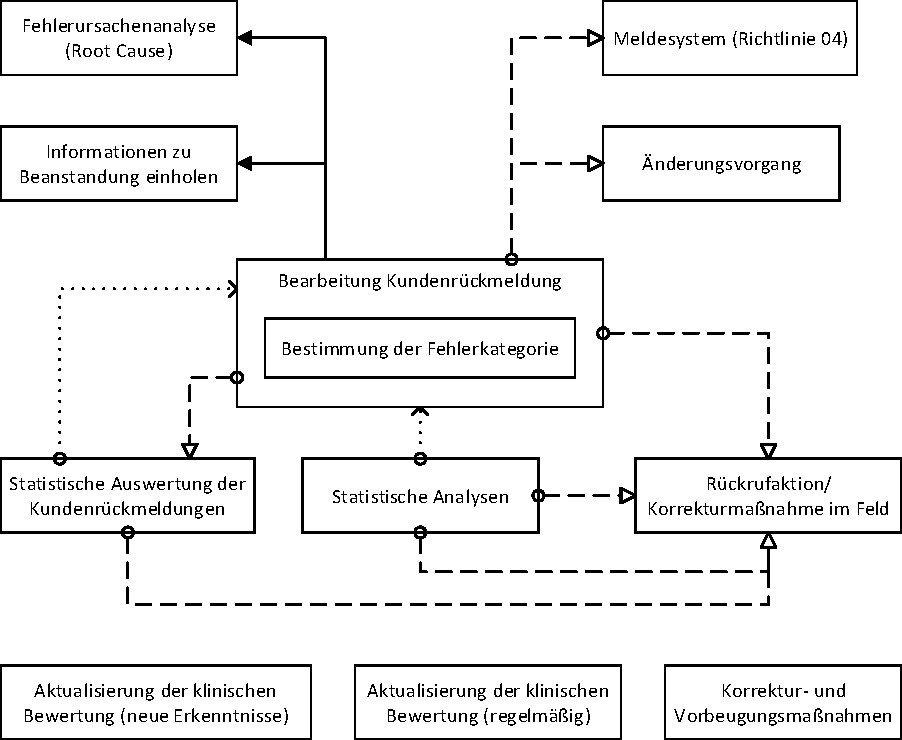
\includegraphics[width=\linewidth,height=\textheight,
keepaspectratio]{Images/process_overview}
\caption[Übersicht über die modellierten Prozesse]{Übersicht über die modellierten Prozesse}
\label{process_overview}
\end{figure}
%===================================================================== Cahpter 4
\chapter{Anpassung des Prozesses unter Berücksichtigung der Medizinprodukteverordnung}\label{chap:AnpassungAnMDR}
Im vorangegangenen Kapitel wurden die aktuellen Prozesse nach dem Inverkehrbringen der Produkte analysiert und mittels BPMN 2.0 in eine grafische Darstellung überführt. Wie bereits in Kapitel \ref{sec:RegRequ} vorgestellt wurde, bestehen für den Medizinproduktmarkt spezielle Anforderungen in Form von regulatorischen Bestimmungen. Für den europäischen Raum wurde im Jahr 2017 mit der MDR eine neue Verordnung erlassen, die viele neue Anforderungen stellt. Die im Rahmen dieser Arbeit betrachteten Prozesse sind mit am stärksten von den Neuerungen betroffen, da in den bisherigen Verordnungen vergleichsweise wenige Pflichten der Hersteller formuliert wurden, beziehungsweise die gegebenen Forderungen großen Spielraum zuließen. Die meisten der Forderungen werden in "`Kapitel VII: Überwachung nach dem Inverkehrbringen, Vigilanz und Marktüberwachung"' formuliert, aber speziell die Anforderungen an die klinische Nachbeobachtung nach dem Inverkehrbringen verteilen sich über einige einzelne Artikel in der MDR.

Für WOM besitzt die Erfüllung der neuen Norm eine hohe Bedeutung, da dies nach Ablauf der Übergangsfristen über die künftige Zulassung von neuen Geräten entscheidet. Im folgenden Kapitel wird deswegen die MDR auf ihre Anforderungen bezogen auf das gewählte Themengebiet untersucht, um im Anschluss den Erfüllungsgrad der Anforderungen zu ermitteln. Am Ende wird ein Vorschlag für die Prozessanpassung erarbeitet, mit dem WOM dem neuen Standard gerecht werden kann.
\section{Ermittlung der Anforderungen der MDR}
Die MDR ist eine durch den Europäischen Rat verabschiedete Verordnung und besitzt folglich Gesetzescharakter, der sich sowohl in der Struktur als auch in den Formulierungen widerspiegelt. Die Ermittlung, ob alle Anforderungen erfüllt werden, gestaltet sich somit schwierig. Die Hauptgründe dafür sind in der thematisch orientierten Struktur, die einen starken Kontrast zum prozessorientierten Blickwinkel von Unternehmen darstellt, und den vielen Querverweisen und Redundanzen, die sich vermutlich aus dem Anspruch ergeben, dass jeder Artikel in sich geschlossen ist und alle für das Verständnis notwendigen Informationen beinhaltet, zu sehen. Thematisch eng zusammenhängende Sachverhalte sind häufig über mehrere Artikel verteilt, was es erschwert, den Zusammenhang zu erfassen und somit einen allumfassenden Blick zu gewinnen. Zudem sind nicht alle Informationen für WOM relevant, da beispielsweise für die angesprochenen Gerätetypen keine entsprechenden Geräte im Portfolio bestehen oder Anforderungen formuliert werden, die vorrangig in den Aufgabenbereich der Behörden fallen und somit keine Aktionen bei den Herstellern erfordern. Diese zusätzlichen Informationen müssen folglich herausgefiltert werden, was zusätzliche Sorgfalt erfordert.

Um dem Anspruch der systematischen Arbeitsweise gerecht zu werden und das Verständnis und die Nachvollziehbarkeit für die zu erzielenden Arbeitsergebnisse sicherzustellen, wird beschlossen, vor der eigentlichen Einschätzung und Analyse der Deckungsgleichheit der Prozesse bei WOM mit den Forderungen der MDR eine ausgiebige Analyse der MDR vorzuschalten. Dies hat zum Ziel jeden relevanten Artikel auf seinen für WOM wesentlichen Anteil zu komprimieren und in eine Anforderungsform zu überführen. Dazu wird jeder Artikel einzeln analysiert und konkrete Anforderungen an die Unternehmensprozesse bei WOM extrahiert. Zur Veranschaulichung dieses Vorgehens soll Artikel 84 dienen, der im Originaltext der MDR folgendermaßen lautet:
\begin{quote}
Das System zur Überwachung nach dem Inverkehrbringen gemäß Artikel 83 stützt sich auf einen Plan zur Überwachung nach dem Inverkehrbringen; die für diesen Plan geltenden Anforderungen sind in Anhang III Abschnitt 1.1 dargelegt. Bei Produkten, die keine Sonderanfertigungen sind, ist der Plan zur Überwachung nach dem Inverkehrbringen Teil der technischen Dokumentation gemäß Anhang II.
\end{quote}
Nach eingehender Analyse können die folgenden Anforderungen extrahiert werden:
\begin{itemize}
\item Plan zur Überwachung nach dem Inverkehrbringen muss erstellt werden
\item Plan ist Teil der technischen Dokumentation (außer bei Sonderanfertigungen)
\end{itemize}
Um die Nachvollziehbarkeit zu erhöhen und einen Überblick zu ermöglichen, werden diese ermittelten Anforderungen in einer zusammenfassenden Liste vereint. Dabei wird über Gruppierung und Clusterung von Anforderungen und Auslöschung von Redundanzen (z.B. in Form von Verweisen und Wiederholungen) eine zusammenfassende Anforderungsliste generiert, die die Analyse der Unternehmensprozesse erleichtern sollte. Das Ergebnis ist eine Checkliste, mit der der Erfüllungsgrad transparent festgestellt werden kann. Dieses Ergebnis ist in Tabelle \ref{tab:MDRRequAndRef} zu erkennen. Über die zweite Spalte ist es weiterhin möglich nachzuvollziehen, aus welchen Artikeln und Absätzen die einzelnen Anforderungen abgeleitet wurden, was die Transparenz und Nachvollziehbarkeit sicherstellt und somit den Nutzen für WOM maximiert.

\def\requestListTabHead{\begin{table}[ht] \centering \begin{tabular}{|p{0.84\textwidth}|p{0.1\textwidth}|} \hline\vspace{0mm} Anforderung & \vspace{0mm}Art.\\ \hline\hline}
\def\ListTabBottom{\end{tabular}\end{table}}
\def\ListTabBottomWithCaptionAndLabel#1#2#3{\end{tabular}\caption[#1]{#2}\label{#3}\end{table}}
\def\plainTabularText#1#2{\begin{tabular}{p{13,6cm}}#1 \\\end{tabular} & \begin{tabular}{p{1cm}}#2 \\\end{tabular}\\}
\def\tabularitemizeFirstLayer#1#2{\begin{tabular}{p{0,3cm}p{12,9cm}}\textbullet & #1 \\\end{tabular} & \begin{tabular}{p{1cm}}#2 \\\end{tabular}\\}
\def\tabularitemizeSecondLayer#1#2{\begin{tabular}{p{0,3cm}p{0,3cm}p{12,1cm}}& - & #1 \\\end{tabular} & \begin{tabular}{p{1cm}}#2 \\\end{tabular}\\}
\def\tabularitemizeSecondLayerUncheck#1{\begin{tabular}{p{0,3cm}p{0,3cm}p{12,7cm}}& - & #1 \\\end{tabular} & \unchecked\\}

\afterpage{
\requestListTabHead
\plainTabularText{System zur Überwachung nach dem Inverkehrbringen (als integraler Bestandteil des QMS) muss eingerichtet sein, angewendet, instandgehalten und dauernd aktualisiert werden}{83/1 83/2}
\hline
\plainTabularText{Plan zur Überwachung nach dem Inverkehrbringen:}{}
\tabularitemizeFirstLayer{Für die Überwachung nach dem Inverkehrbringen muss ein Plan erstellt werden, der Teil der technischen Dokumentation ist (außer bei Sonderanfertigungen}{84}
\tabularitemizeFirstLayer{Enthält u.A. Vorgehen, wie Trends erkannt werden (Methodik), zu behandeln sind und wie der Beobachtungszeitraum festgelegt wird}{88/1}
\hline
\plainTabularText{Es werden Daten über Qualität, Leistung und Sicherheit eines Produktes während gesamter Lebensdauer gesammelt, aufgezeichnet, analysiert und verwendet für:}{83/2 83/3}
\tabularitemizeFirstLayer{Aktualisierung des Risikomanagements}{83/3}
\tabularitemizeFirstLayer{Aktualisierung der GA, Informationen zur Herstellung und Kennzeichnung}{83/3}
\tabularitemizeFirstLayer{Aktualisierung der klinischen Bewertung}{83/3}
\tabularitemizeFirstLayer{Aktualisierung Kurzbericht über Sicherheit und klinische Leistung (für Klasse III Geräte)}{83/3}
\tabularitemizeFirstLayer{Ermittlung des Bedarfs an Präventiv-, Korrektur- oder Sicherheitskorrekturmaßnahmen im Feld}{83/3}
\tabularitemizeFirstLayer{Ermittlung von Möglichkeiten zur Verbesserung der Gebrauchstauglichkeit, der Leistung und der Sicherheit des Produkts}{83/3}
\tabularitemizeFirstLayer{Gegebenenfalls Beitrag zur Überwachung anderer Produkte nach dem Inverkehrbringen}{83/3}
\tabularitemizeFirstLayer{Erkennung und Meldung von Trends}{83/3}
\plainTabularText{Die Technische Dokumentation ist immer aktuell zu halten}{83/3}
\hline
\plainTabularText{Durchführung und Überwachung von Präventiv- und Korrekturmaßnahmen aufgrund von gesammelten Daten inklusive Unterrichtung der zuständigen Behörden und gegebenenfalls benannter Stelle durch den Hersteller, bei schwerwiegenden Vorkommnissen und notwendigen Sicherheitskorrekturmaßnahmen im Feld}{83/4}
\hline
\plainTabularText{Schwerwiegende Vorkommnisse oder Sicherheitskorrekturmaßnahmen im Feld:}{}
\tabularitemizeFirstLayer{Schwerwiegende Vorkommnisse, die im Zusammenhang zum Produkt stehen, werden den Behörden über elektronisches System gemeldet, außer es sind erwartete Nebenwirkungen laut Produktinformation, in technischer Dokumentation quantifiziert und durch Meldung von Trends erfasst}{87/1 92/1}
\tabularitemizeSecondLayer{Meldung innerhalb 2 Tage nach Kenntnis der Gefahr, wenn schwerwiegende Gefahr für öffentliche Gesundheit besteht}{87/4}
\tabularitemizeSecondLayer{Meldung innerhalb 10 Tage nach Kenntnis des Vorkommnisses, wenn Tod oder unvorhergesehener Verschlechterung des Gesundheitszustandes einer Person und Kausalzusammenhang zum Produkt besteht oder vermutet wird}{87/5}
\hline
\ListTabBottom

\requestListTabHead
\tabularitemizeSecondLayer{Meldung innerhalb 15 Tage nach Kenntnis des Vorkommnisses, wenn Kausalzusammenhang zwischen Produkt und Vorkommnis festgestellt wurde oder möglich ist}{87/3}
\hline
\plainTabularText{Schwerwiegende Vorkommnisse oder Sicherheitskorrekturmaßnahmen im Feld:}{}
\tabularitemizeFirstLayer{Schwerwiegende Vorkommnisse, die im Zusammenhang zum Produkt stehen, werden den Behörden über elektronisches System gemeldet, außer es sind erwartete Nebenwirkungen laut Produktinformation, in technischer Dokumentation quantifiziert und durch Meldung von Trends erfasst}{87/1 92/1}
\tabularitemizeSecondLayer{Meldung innerhalb 2 Tage nach Kenntnis der Gefahr, wenn schwerwiegende Gefahr für öffentliche Gesundheit besteht}{87/4}
\tabularitemizeSecondLayer{Meldung innerhalb 10 Tage nach Kenntnis des Vorkommnisses, wenn Tod oder unvorhergesehener Verschlechterung des Gesundheitszustandes einer Person und Kausalzusammenhang zum Produkt besteht oder vermutet wird}{87/5}
\tabularitemizeSecondLayer{Meldung innerhalb 15 Tage nach Kenntnis des Vorkommnisses, wenn Kausalzusammenhang zwischen Produkt und Vorkommnis festgestellt wurde oder möglich ist}{87/3}
\tabularitemizeFirstLayer{Sicherheitskorrekturmaßnahmen im Feld, auch wenn Vorkommnis außerhalb der EU aufgetreten ist, aber Grund für Maßnahme direkt von einem Produkt, das auch in EU gehandelt wird, ausgeht, werden den zuständigen Behörden über elektronisches System gemeldet}{87/1 92/1}
\tabularitemizeSecondLayer{Meldung über Sicherheitskorrekturmaßnahme im Feld in nicht dringenden Fällen ohne gebührliche Verzögerung vor der Durchführung}{87/8}
\tabularitemizeSecondLayer{Bei wiederholenden Meldungen (ähnliches Vorkommnis mit gleichem Produkt oder Produktart,  schon erfolgter Sicherheitskorrekturmaßnahme oder häufig auftretend aber gut dokumentiert) kann periodische Sammelmeldung über elektronisches System erfolgen}{87/9 92/1}
\tabularitemizeFirstLayer{Untersuchung  (u.A. Risikobewertung) folgt unverzüglich auf Meldung eines schwerwiegenden Vorkommnisses durch den Hersteller}{89/1}
\tabularitemizeSecondLayer{Zusammenarbeit gegebenenfalls mit Behörden und benannter Stelle}{89/1}
\tabularitemizeSecondLayer{Untersuchung muss sicherstellen, dass spätere Bewertung der Ursache des Vorkommnisses noch möglich ist oder Maßnahmen, die dagegen verstoßen würden, müssen vorher mit Behörde abgesprochen werden}{89/1}
\tabularitemizeFirstLayer{Notwendige Unterlagen müssen bei entsprechenden Anfragen an die Behörden ausgehändigt werden}{89/3}
\tabularitemizeFirstLayer{Erstellung eines Abschlussberichtes (enthält Schlussfolgerungen und gegebenenfalls zu ergreifende Korrekturmaßnahmen) und Einreichung über elektronisches System}{89/5}
\tabularitemizeFirstLayer{Bei ergriffenen Sicherheitskorrekturmaßnahmen im Feld müssen die Anwender mittels Sicherheitsanweisung im Feld über elektronisches System informiert werden}{89/8 92/1}
\hline
\ListTabBottom

\requestListTabHead
\tabularitemizeSecondLayer{Entwurf der Anweisung wird koordinierender zuständiger Behörde vorgelegt (außer in dringenden Fällen), damit diese Anmerkungen abgeben kann}{89/8}
\tabularitemizeSecondLayer{Identifikation über UDI und SRN}{89/8}
\tabularitemizeSecondLayer{Enthalten sind Gründe für Sicherheitskorrekturmaßnahme im Feld mit Verweis auf Fehlfunktion und Risiken für Patienten, Anwender oder Dritte sowie alle zu ergreifenden Maßnahmen}{89/8}
\tabularitemizeFirstLayer{Information über mögliche schwerwiegende Vorkommnisse können von zuständiger Behörde kommen, sofern diese zuerst informiert wurde}{87/11}
\tabularitemizeSecondLayer{Behörde kann vom Hersteller Schritte gemäß schwerwiegendem Vorkommnis einfordern, auch wenn dieser ermittelt hat, dass Vorfall nicht schwerwiegend ist oder es als erwartete, unerwünschte Nebenwirkung, die in der Meldung von Trends enthalten sein wird, klassifiziert}{87/11}
\hline
\plainTabularText{Bericht zur Überwachung nach dem Inverkehrbringen/Sicherheitsbericht:}{}
\tabularitemizeFirstLayer{Klasse I:}{}
\tabularitemizeSecondLayer{Zur Zusammenfassung der Überwachung nach dem Inverkehrbringen und der ergriffenen Präventiv- und Korrekturmaßnahmen (Beschreibung und Begründung der Maßnahmen) muss ein Bericht erstellt werden}{85}
\tabularitemizeFirstLayer{Klasse IIa, IIb, III:}{}
\tabularitemizeSecondLayer{Ergebnisse und Schlussfolgerunge der PMS sowie Beschreibung und Begründung ergriffener Präventiv- und Korrekturmaßnahmen müssen enthalten sein (erstellt pro Produkt, gegebenenfalls Produktkategorie oder Produktgruppe)}{86/1}
\tabularitemizeSecondLayer{Aktualisierung über gesamte Lebensdauer}{86/1}
\tabularitemizeSecondLayer{Enthält:\newline a) die Schlussfolgerungen aus der Nutzen-Risiko-Abwägung\newline b) die wichtigsten Ergebnisse des Bewertungsberichts\newline c) die Gesamtabsatzmenge des Produkts und eine Schätzung der Anzahl und anderer Merkmale der Personen, bei denen das betreffende Produkt zur Anwendung kommt, sowie, sofern dies praktikabel ist, die Häufigkeit der Produktverwendung}{86/1}
\tabularitemizeFirstLayer{Aktualisierungsintervalle:}{}
\tabularitemizeSecondLayer{Klasse I: bei Bedarf und auf Anfrage der Behörden}{85}
\tabularitemizeSecondLayer{Klasse IIa: mindestens alle 2 Jahre (Teil der technischen Dokumentation)}{86/1}
\tabularitemizeSecondLayer{Klasse IIb: mindestens 1x jährlich (Teil der technischen Dokumentation)}{86/1}
\tabularitemizeSecondLayer{Klasse III: mindestens 1x jährlich (Teil der technischen Dokumentation)}{86/1}
\tabularitemizeFirstLayer{Vorlage des Berichtes:}{}
\tabularitemizeSecondLayer{Klasse I: bei benannter Stelle oder auf Anfrage durch Behörde}{86/3}
\tabularitemizeSecondLayer{Klasse IIa, IIb, Sonderanfertigungen: über elektronisches System bei benannter Stelle oder auf Anfrage durch Behörde}{86/3 92/1}
\hline
\ListTabBottom

\requestListTabHead
\tabularitemizeSecondLayer{Klasse III und implantierbare Produkte: über elektronisches System an benannte Stelle}{86/2 92/1}
\tabularitemizeFirstLayer{Bei Sonderanfertigungen separate Struktur der Dokumentation}{86/1}
\hline
\plainTabularText{Trends:}{}
\tabularitemizeFirstLayer{Meldung von statistisch signifikanten (entscheidend ist Vergleich mit erwartetem und in techn. Doku angegebener Häufung) Anstiegen der Häufigkeit oder des Schweregrades nicht schwerwiegender Vorkommnisse oder erwarteter unerwünschter Nebenwirkungen über elektronisches System, wenn Nutzen-Risiko-Analyse erheblich beeinflusst wird und Risiken für die Gesundheit entstehen}{88/1 92/1}
\tabularitemizeFirstLayer{Behörden können bei abweichender Einschätzung  der Meldung vom Hersteller verlangen, Maßnahmen zu ergreifen}{88/2}
\hline
\plainTabularText{Klinische Nachbeobachtung nach dem Inverkehrbringen
(PMCF):}{}
\tabularitemizeFirstLayer{Ist Teil des Qualitätsmanagementsystems und wird aufgestellt, angewendet, aufrechterhalten und auf dem neuesten Stand gehalten}{10/9}
\tabularitemizeFirstLayer{Prozess der klinischen Nachbeobachtung nach dem Inverkehrbringen aktualisiert klinische Bewertung während gesamter Lebensdauer und ist Teil des Plans zur Überwachung nach dem Inverkehrbringen}{10/3 61/11 XIV/5}
\tabularitemizeFirstLayer{Klinische Daten, die bei zweckgemäßer Verwendung erhoben werden, werden proaktiv gesammelt und ausgewertet, um:}{XIV/5}
\tabularitemizeSecondLayer{Sicherheit und Leistung während der Lebensdauer zu bestätigen}{XIV/5}
\tabularitemizeSecondLayer{Konformität der ermittelten Risiken sicherzustellen}{XIV/5}
\tabularitemizeSecondLayer{Neu entstehende Risiken und Nebenwirkungen auf Grundlage empirischer Belege zu identifizieren}{XIV/5 XIV/6}
\tabularitemizeSecondLayer{Vertretbarkeit Nutzen-Risiko-Verhältnis zu gewährleisten}{XIV/6}
\tabularitemizeSecondLayer{Systematisch fehlerhafte oder zulassungsüberschreitende Verwendung festzustellen (Prüfung auf Angemessenheit der Zweckbestimmung)}{XIV/6}
\tabularitemizeFirstLayer{Ein Plan wird erstellt, der folgendes enthält:}{XIV/6}
\tabularitemizeSecondLayer{Allgemein anzuwendende Methoden und Verfahren zur Erhebung und Begründung der Eignung}{XIV/6}
\tabularitemizeSecondLayer{Verweis auf relevante Teile des Berichts über klinische Bewertung und das Risikomanagement}{XIV/6}
\tabularitemizeSecondLayer{Abzudeckende spezifische Ziele}{XIV/6}
\tabularitemizeSecondLayer{Bewertung der klinischen Daten zu gleichartigen oder ähnlichen Produkten}{XIV/6}
\tabularitemizeSecondLayer{Verweis auf GS (gemeinsame Spezifikation), harmonisierte Normen (wenn angewendet) und einschlägige Leitlinien zum Thema}{XIV/6}
\tabularitemizeSecondLayer{Zeitplan für die geplanten Tätigkeiten}{XIV/6}
\hline
\ListTabBottom

\requestListTabHead
\tabularitemizeFirstLayer{Ergebnisse werden in Bewertungsbericht, der Teil der technischen Dokumentation ist, dokumentiert}{XIV/7}
\tabularitemizeFirstLayer{Schlussfolgerungen werden bei klinischer Bewertung und Risikomanagement berücksichtigt}{XIV/8}
\tabularitemizeFirstLayer{Notwendigkeit zur Durchführung von Präventiv-/ oder Korrekturmaßnahmen im Feld wird ermittelt und Prozesse entsprechend gestartet}{XIV/8}
\tabularitemizeFirstLayer{Durchführung von Studien über klinische Nachbeobachtung nach dem Inverkehrbringen, die von benannten Stelle gefordert werden}{56/3}
\hline
\plainTabularText{Analyseaktivitäten der Behörden:}{}
\tabularitemizeFirstLayer{Unterlagen und Informationen für Behörden zwecks Durchführung der Marktüberwachung zur Verfügung stellen}{93/3}
\tabularitemizeFirstLayer{Produktstichproben oder Zugang zu Produkten bei gerechfertigtem Anliegen den Behörden kostenfrei zur Verfügung stellen}{93/3}
\tabularitemizeFirstLayer{Hersteller ergreift erforderliche Korrekturmaßnahmen, wenn Behörden aus der Analyse der Vigilanz-Daten Risiken oder nachteilige Änderugen der Nutzen-Risiko-Abwägung ermitteln und dem Hersteller mitteilen}{90}
\tabularitemizeFirstLayer{Kooperation bei Bewertung eines Produktes aufgrund des Verdachtes}{94}
\tabularitemizeSecondLayer{Eines unvertretbaren Risikos für die Gesundheit oder Sicherheit oder für Aspekt des Schutzes der öffentlichen Gesundheit}{94}
\tabularitemizeSecondLayer{Anderweitig nicht erfüllte Anforderungen der Verordnung}{94}
\tabularitemizeFirstLayer{Prüfung des durch die Behörde erstellten Berichtes über eine durchgeführte Kontrolle und gegebenenfalls Verfassung einer Stellungnahme durch den Hersteller, die in elektronischem System in Form einer Stellungnahme erfasst wird}{93/7}
\tabularitemizeFirstLayer{Zuständige Behörde kann zu Ergreifung von geeigneten und gebührend gerechtfertigten Korrekturmaßnahmen bei vertretbaren und unvertretbaren Risiken  für die Gesundheit oder Sicherheit der Patienten, Anwenders oder anderer Personen oder in Bezug auf andere Aspekte des Schutzes der öffentlichen Gesundheit auffordern, um Konformität des Produkts herzustellen (Bereitstellung des Produktes, die der Art des Risikos angemessen ist, Beschränkung des Risikos, Bereitstellung des Produktes bestimmten Anforderungen unterwerfen, Produkt vom Markt nehmen, Produkt zurückrufen)}{95/1 97/1}
\tabularitemizeSecondLayer{Notwendige Korrekturmaßnahme in gesamter europäischer Union durchführen, wo betroffenes Produkt auf dem Markt verfügbar ist}{95/3}
\tabularitemizeFirstLayer{Unterstützung der Kommission, bei der Überprüfung der Rechtmäßigkeit von getroffenen Maßnahmen eines Mitgliedsstaates, wenn Einwände eines anderen Mitgliedsstaates dagegen bestehen oder Kommission die Maßnahme für nicht mit dem Unionsrecht vertretbar einschätzt, in Form von Anhörungen}{96/1}
\tabularitemizeFirstLayer{Unterstützung der Kommission in Form von Absprache zur Prüfung getroffener Maßnahmen nationaler Behörden, wenn erforderlich}{98/3}
\hline
\ListTabBottomWithCaptionAndLabel{Anforderungsliste aus MDR mit Referenzen}{Anforderungsliste aus MDR mit Referenzen}{tab:MDRRequAndRef}
\clearpage
}

\section{Analyse der momentan verwendeten Prozesse}
Nachdem der Anforderungskatalog aus der MDR extrahiert wurde, können die aktuellen Prozesse analysiert werden, wobei die Erfüllung jeder einzelnen Anfrage geprüft wird. Dazu wird die Anforderungstabelle aus Tabelle \ref{tab:MDRRequAndRef} in eine Checkliste überführt, indem die Spalte mit den Referenzen auf die Artikel der MDR durch eine Spalte mit Checkboxen, die den aktuellen Status der Erfüllung darstellen, ersetzt wird (siehe Anhang \ref{chap:ChecklistMDR}).

Es zeigt sich, dass nicht alle Anforderungen erfüllt werden, was aufgrund komplett neuer Anforderungen logisch erscheint. Das elektronische System, was von den Behörden als zentrale Informationsplattform zur Verfügung gestellt wird und die Verwendung dessen stellen eine der Hauptquellen für nicht erfüllte Anforderungen dar, da diese allesamt neu sind. Des Weiteren wurden die Fristen des Meldesystems der Hersteller deutlich nachgeschärft, wodurch neue striktere Fristen eingeführt wurden, die ebenfalls nicht erfüllt werden. 

Generell gilt, dass die Tätigkeiten und Aktivitäten der Behörden eine wichtige Rolle in der MDR spielen, wodurch sich einige Anforderungen für den Hersteller aus den möglichen Aktionen der Behörden ergeben. Diese können beispielsweise Korrekturmaßnahmen oder Untersuchungen einfordern, was in den aktuellen Prozessen noch nicht berücksichtigt ist. Speziell die passive Interaktion mit den Behörden (z.B. in Form von Reaktion auf Anfragen der Behörden) ist in den momentanen Prozessen nicht erschlossen, was in der Praxis zu Abstimmungsschwierigkeiten führen könnte, da nicht genau geregelt ist, welche Stelle sich um die Bearbeitung einer Anfrage von außen kümmern soll.

Ebenfalls nicht umgesetzt sind die Meldung von Trends und die Erstellung eines Plans für die Aktivitäten zur Marktbeobachtung nach dem Inverkehrbringen. Letzteres spielt zwar eine wichtige Rolle für die Erfüllung der Forderungen der MDR, da durch den Plan der Grundstein der Überwachung gelegt wird. Trotzdem wird dieser Sachverhalt nicht im Rahmen dieser Arbeit betrachtet, da dieser Prozess noch vor dem Inverkehrbringen abläuft und somit den gewählten Betrachtungshorizont übersteigt.

Mit der Schärfung der Anforderungen für die Aktualisierung der klinischen Bewertung nach dem Inverkehrbringen durch die klinische Nachbeobachtung nach dem Inverkehrbringen (PMCF) sind ebenfalls neue Aufgaben für die Hersteller festgelegt worden. Auch in diesem Falle wurden die Anforderungen für den europäischen Raum durch die MDR klarer formuliert, wodurch sich für die Hersteller neue Erfüllungskriterien ergeben. Zu den nicht erfüllten Aufgaben zählt die Erstellung eines Planes zur Überwachung, der Teil des Plans zur Überwachung nach dem Inverkehrbringen ist. Da dieser, wie bereits erwähnt wurde, nicht in den Fokus dieser Arbeit fällt, bleibt auch die Forderung für den PMCF-Plan unbeachtet. Des Weiteren werden einige Forderungen in der Praxis zwar schon gelebt, aber in den Unterlagen des QM-Handbuches nicht aufgeführt. Dazu gehört die Einbeziehung der Erkenntnisse der klinischen Bewertung in der Risikobeurteilung sowie die Ableitung von Korrekturmaßnahmen oder Rückrufen aus den neuen Erkenntnissen. Auch die Rolle der benannten Stelle wird in der MDR gestärkt, da diese nun auch klinische Studien von den Herstellern einfordern kann, worauf in den Verfahrensanweisungen und den Richtlinien aktuell nicht verwiesen wird.
\section{Prozessanpassung aufgrund nicht erfüllter Anforderungen der MDR}
Wie bereits angesprochen wurde, führen nicht alle offenen Anforderungen zu tatsächlichen Anpassungen an den ermittelten Prozessen. Dies liegt vor allem daran, dass die anzupassenden Prozesse nicht modelliert wurden und somit nicht Bestandteil der Prozesse nach dem Inverkehrbringen sind. Generell stellen die hier erarbeiteten Prozesse nur eine Möglichkeit vor, wie die Anforderungen mit möglichst wenig Aufwand umgesetzt werden können. Die tatsächliche Lösung könnte im Nachhinein aufgrund von Firmenbelangen anders aussehen. Grafische Vorher-Nachher-Vergleiche drängen sich an dieser Stelle nahezu auf, aber aufgrund der Zerstreuung der durchgeführten Änderungen in einer großen Prozesslandkarte macht es nur an wenigen Stellen Sinn, einen entsprechenden plakativen Vergleich aufzuzeigen.

Die größte Anpassung betrifft den Prozess der Kundenrückmeldung, der im bisherigen Modell den umfangreichsten und zentralsten Prozess im Kontext der Marktbeobachtung nach dem Inverkehrbringen darstellt. Kundenrückmeldungen dienten somit als einzige richtige Quelle für PMS, was nach den Anforderungen der MDR zu wenig ist. Die in dem Prozess enthaltenen Aktivitäten zur Untersuchung und Bearbeitung von Vorkommnissen und Fehlern soll erhalten bleiben und für weitere Vorkommnisse, die nicht über Kundenrückmeldungen eingesteuert wurden, verwendet werden. Mit anderen Worten wird der Prozess allgemeingültiger. Dafür wird er zunächst in "`PMS"' umbenannt, was den thematischen Rahmen für den Prozess festlegt. In der Folge werden alle Tätigkeiten, die sich mit der eigentlichen Bearbeitung der Kundenrückmeldung beschäftigen, abstrahiert, um weitere Quellen für den Untersuchungs- und Bearbeitungsprozess zu ermöglichen. Der aktuelle Prozess wird folglich aufgespalten und es entsteht ein separater Prozess, der sich mit der Aufnahme und Bearbeitung einer Kundenrückmeldung beschäftigt. In diesem separaten Prozess wird der PMS-Prozess bei Bedarf ausgelöst, was sich auch an den Startbedingungen des PMS-Prozess erkennen lässt. 

Neben den Kundenrückmeldungen gibt es die Möglichkeit, dass im Rahmen einer Instanz des PMS-Prozesses (für ein Vorkommnis von einem Gerät) festgestellt wird, dass das Vorkommnis oder der Fehler auch für andere Geräte relevant ist, weswegen eine weitere Instanz des PMS-Prozesses gestartet wird. Dafür wird ein zusätzliches Startereignis einmodelliert. Zudem können die Behörden auch über Vorkommnisse informieren oder von den Unternehmen spezielles Verhalten einfordern, was als Startereignisse für den PMS-Prozess hinzugefügt wird. Im letzten Fall können die Behörden sogar konkrete Maßnahmen vom Hersteller einfordern, wodurch die Fehleruntersuchung und die Schnittstelle zum Meldesystem für diesen Fall obsolet wird. Dies äußert sich im Prozess darin, dass die entsprechenden Prozessabschnitte übersprungen werden und zeitnah nach der Information durch die Behörde mit der Bearbeitung der geforderten Maßnahmen begonnen werden kann. Eine Übersicht über die Startereignisse des angepassten PMS-Prozesses kann Abbildung \ref{pms_process_starts} entnommen werden.
\begin{figure}[ht]
\centering
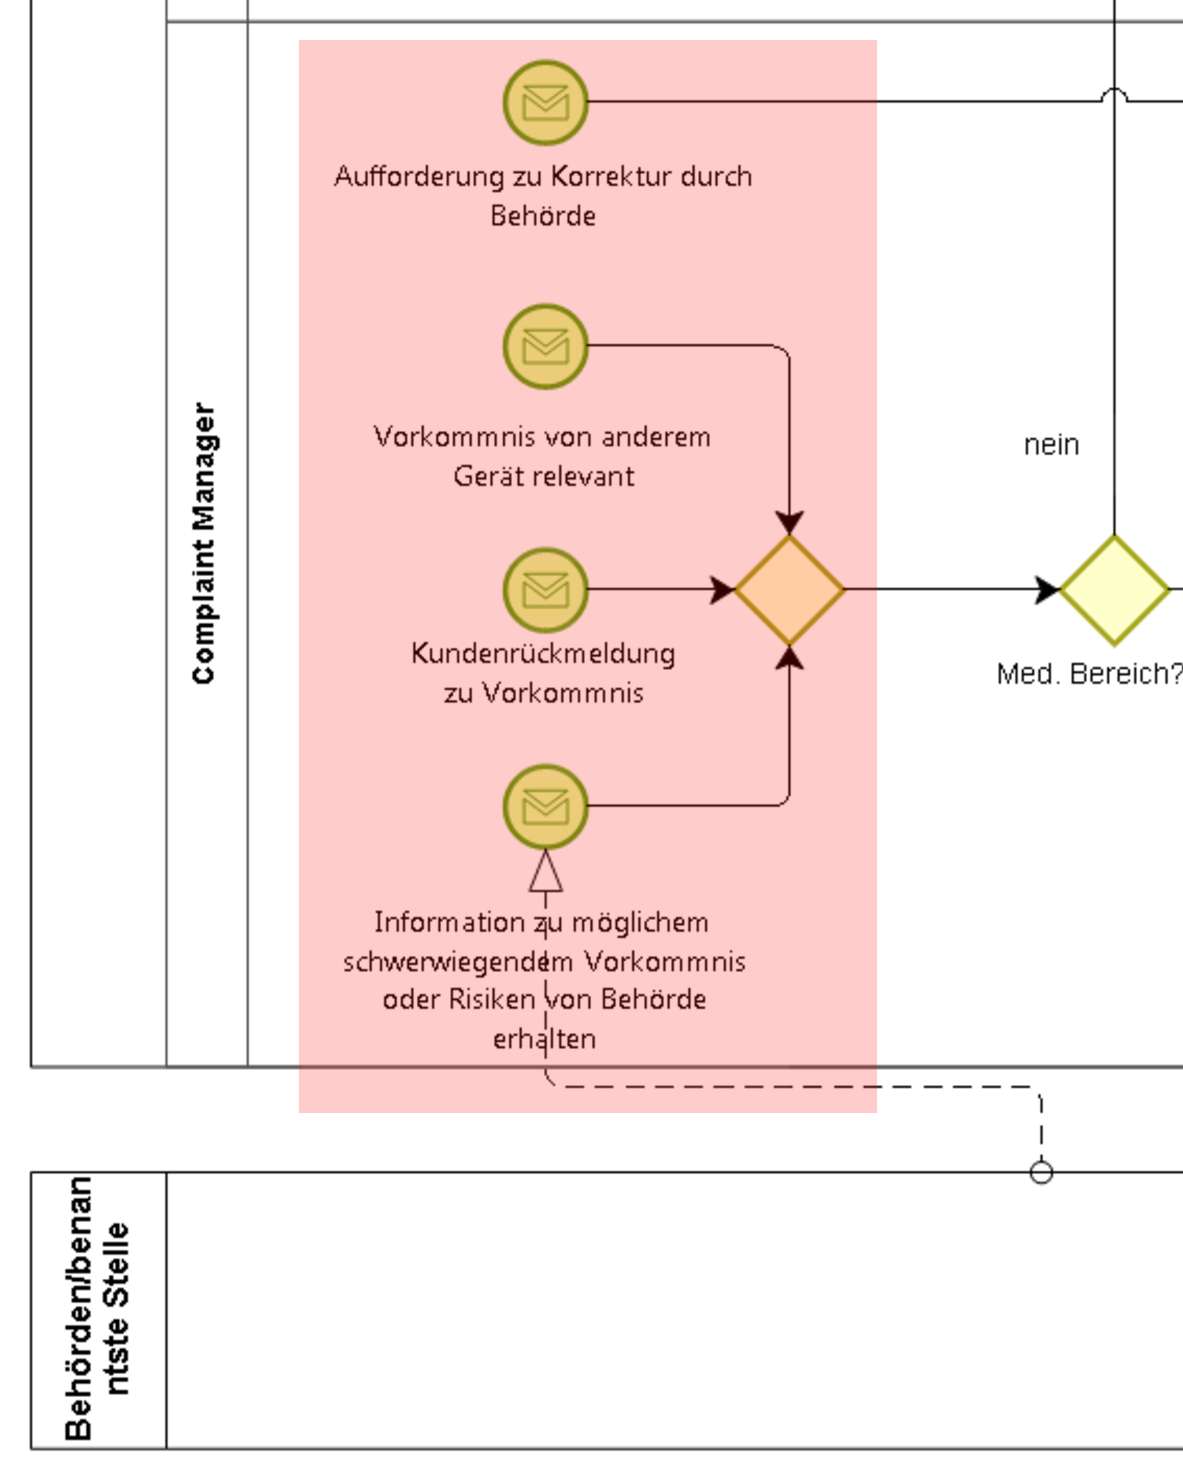
\includegraphics[width=0.6\textwidth]{Images/pms_process_starts}
\caption[Übersicht über die Startereignisse des angepassten PMS-Prozess]{Übersicht über die Startereignisse des angepassten PMS-Prozess}
\label{pms_process_starts}
\end{figure}

Für das Meldesystem gibt es ebenfalls einige Anpassungen. Zum einen gibt es deutliche Veränderungen bei den Fristen für die Einreichung von Meldungen, die nach der neuen Verordnung wesentlich straffer sind. Zum anderen hat sich auch die Form der Einreichung verändert, da hierfür ein durch die europäische Kommission und die Mitgliedsstaaten eingerichtetes elektronisches System verwendet werden soll. Da bereits im bestehenden Prozess bei bestehender Verantwortung durch WOM die Mitteilung an die Behörden gesendet wurde, muss der Prozess nicht wesentlich verändert werden. Es müssen lediglich Hinweise für die einzuhaltenden Fristen in Abhängigkeit von der Brisanz des zu meldenden Vorkommnis und ein Verweis auf das elektronische System eingefügt werden. Zudem bietet die MDR die Möglichkeit, bei Fehlern, die sich über mehrere Geräte oder Gerätegruppen erschließen, eine Sammel-/Wiederholungsmeldung durchzuführen, was den bürokratischen Aufwand für den Hersteller und die Behörden minimieren sollte. Hierbei handelt es sich jedoch um eine optionale Möglichkeit, die nicht notwendigerweise umgesetzt werden muss und demnach bei den Änderungen nicht berücksichtigt wird.

Das elektronische System für die Einreichung von Meldungen und Informationen betrifft auch den Prozess des Rückrufs und der Korrekturmaßnahmen im Feld, da der darin erstellte Abschlussbericht über die durchgeführten Aktionen über das elektronische System eingereicht werden muss. Zudem wird die Information an die Kunden nicht mehr individuell nach den Vorgehensweisen des Unternehmens weitergeleitet, sondern über das elektronische System zentral koordiniert. Dabei wird die durch den Hersteller einzureichende Sicherheitsanweisung im Feld zunächst von den Behörden geprüft, bevor sie über das elektronische System eingereicht wird und somit verfügbar ist. Dieser Teilprozess wird in den Prozess für Rückruf und Korrekturmaßnahmen im Feld eingefügt und ist in Abbildung \ref{recall_message_for_customers} einzusehen.
\begin{figure}[ht]
\centering
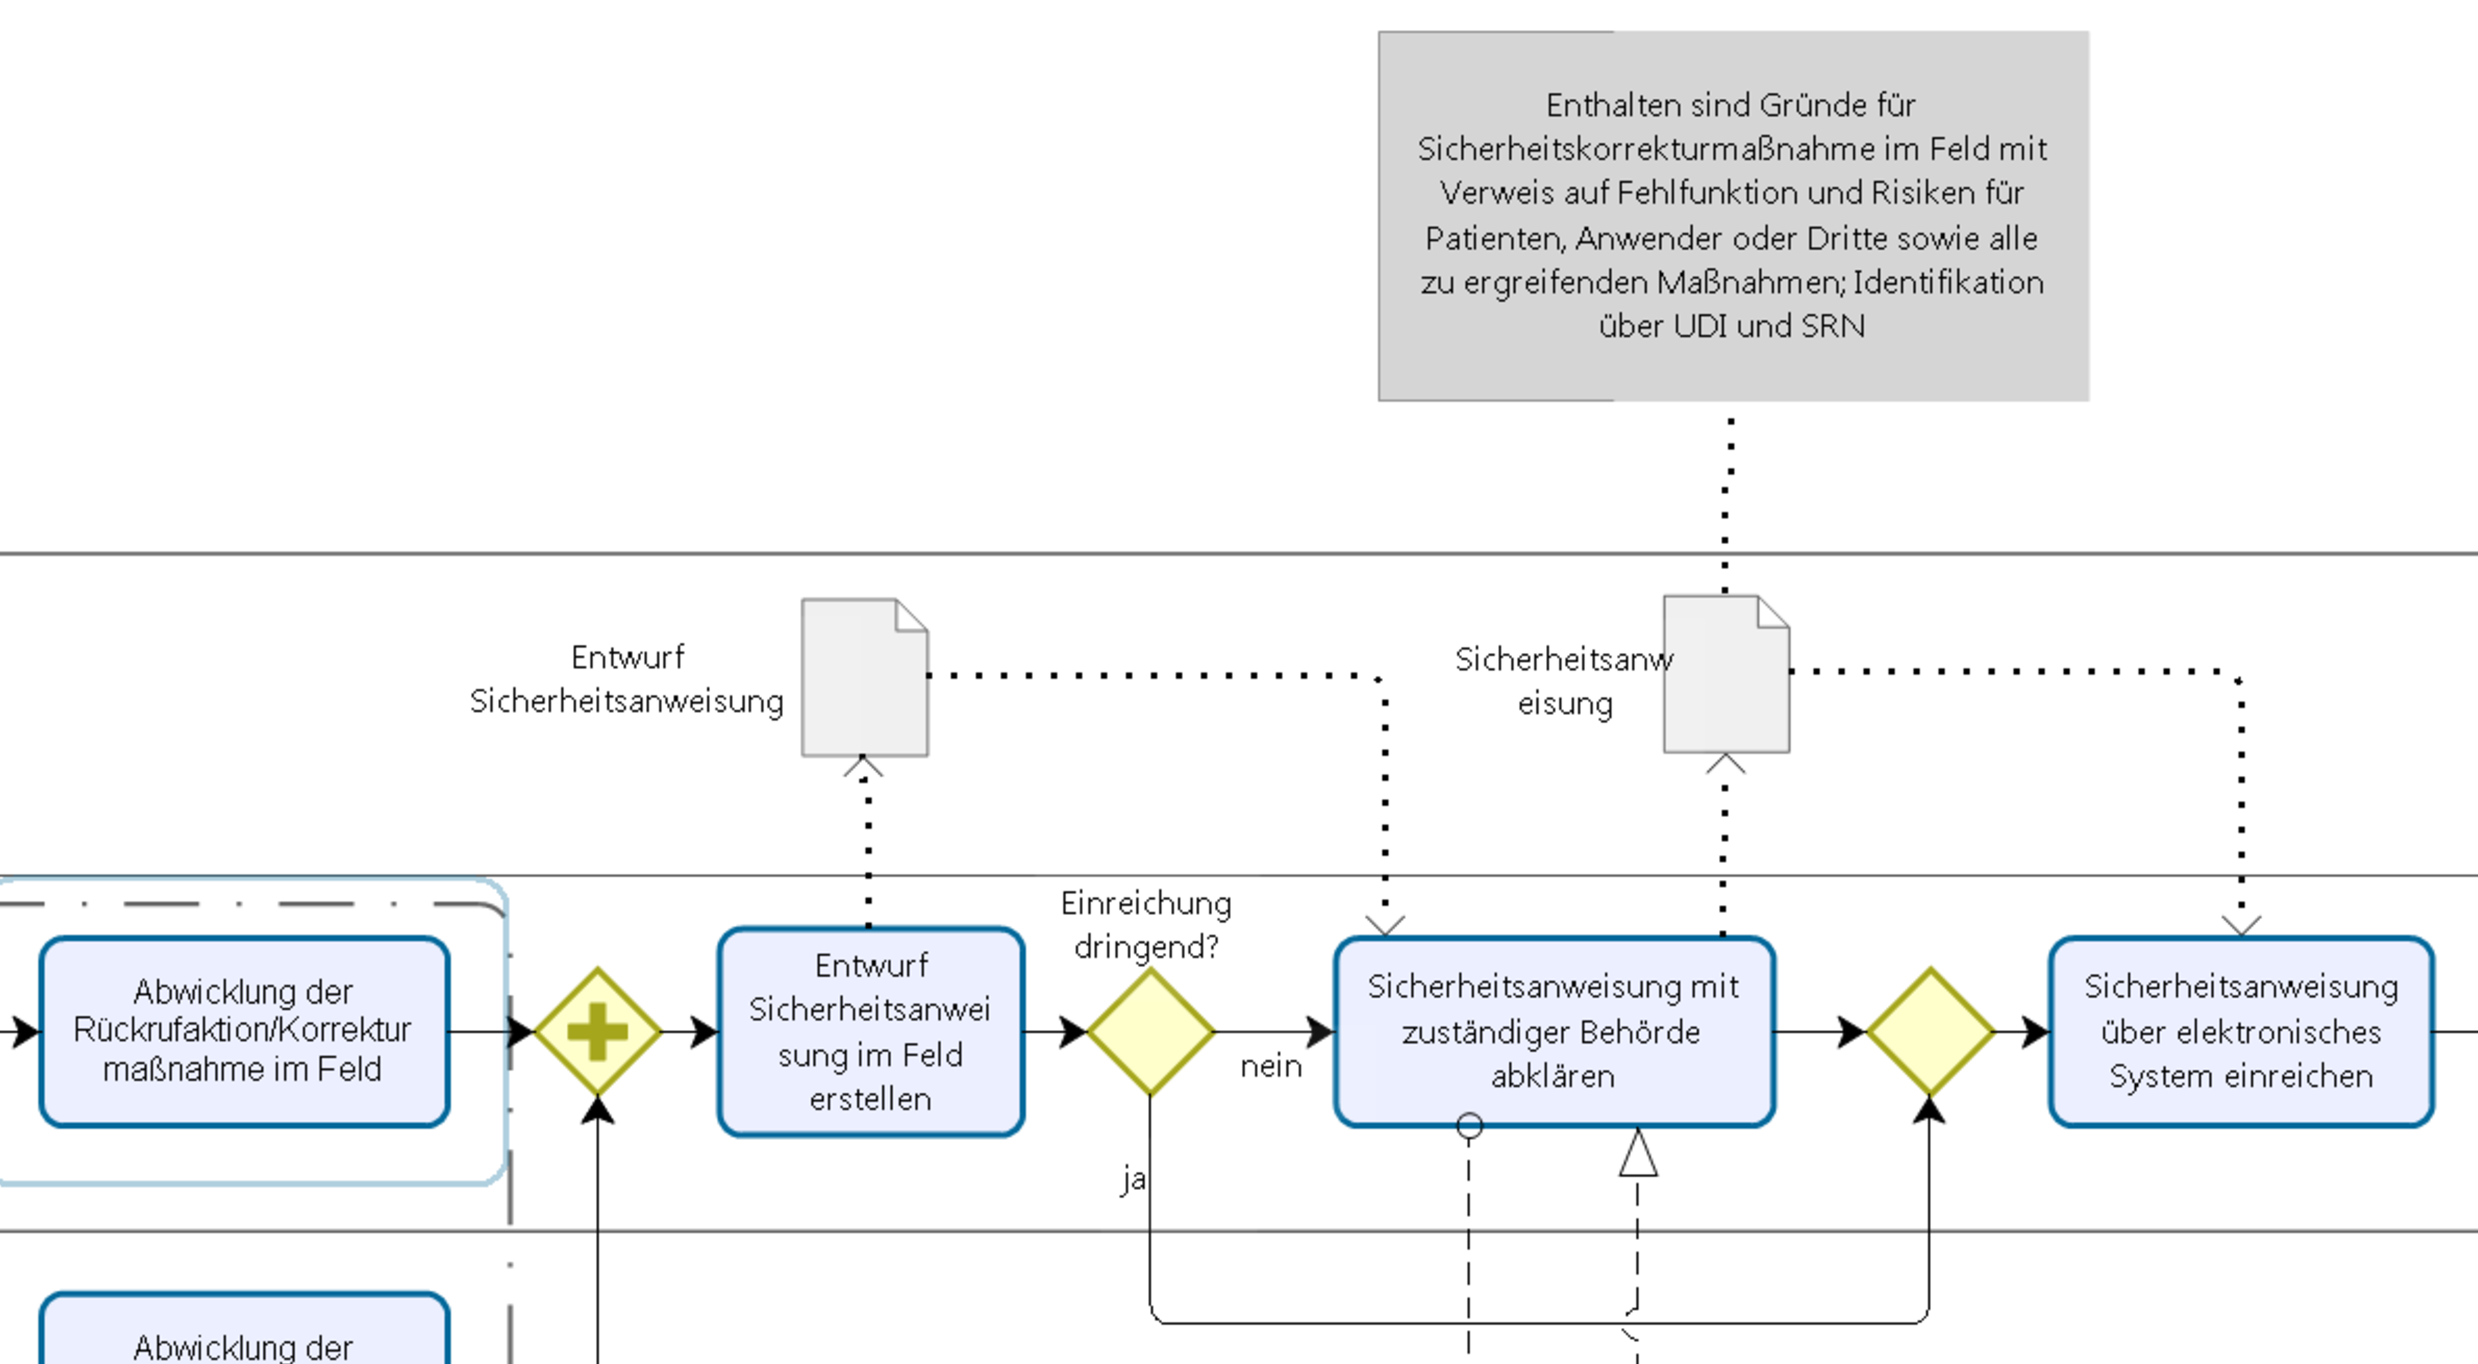
\includegraphics[width=1\textwidth]{Images/recall_message_for_customers}
\caption[Anpassungen im Prozess für Rückruf und Korrekturmaßnahmen im Feld]{Anpassungen im Prozess für Rückruf und Korrekturmaßnahmen im Feld}
\label{recall_message_for_customers}
\end{figure}

Auch die klinische Bewertung, genauer gesagt die klinische Nachbeobachtung nach dem Inverkehrbringen, muss angepasst werden, da einige Anforderungen nicht umgesetzt sind. Dabei halten sich die Änderungen jedoch in Grenzen, da der aktuelle Prozess viele Forderungen bereits abdeckt. Zu den durchzuführenden Änderungen gehört das Hinzufügen der durch die MDR angesprochenen Rückwirkung auf das Risikomanagement, das durch einen zusätzlichen Hinweis, der an den Bewertungsbericht angehängt wird, erfüllt wird. Außerdem wird nach Abschluss der Bewertung geprüft, ob Rückruf- oder Korrekturmaßnahmen im Feld nötig sind und diese bei Bedarf ausgelöst. Als letzter Punkt muss die Möglichkeit, dass durch die benannte Stelle die Durchführung von klinischen Studien gefordert werden kann, berücksichtigt werden. Dazu wird ein zusätzliches Startereignis für den Prozess modelliert, das bei einer entsprechenden Meldung der benannten Stelle den gesamten Prozess startet. Im späteren Verlauf wird dann ermittelt, ob eine zusätzliche klinische Validierung notwendig ist, die für diesen Fall entsprechend durchgeführt wird.

Eine weitere Neuerung ist die konsequente Einforderung von Trendanalysen durch den Hersteller, wonach bei entsprechenden Auffälligkeiten Meldungen an die Behörden abgesetzt werden müssen und unter Umständen Korrektur- und Sicherheitsmaßnahmen durchgeführt werden müssen. Diese Trendanalysen sind in der geforderten Form bei WOM noch nicht vorhanden. Thematisch passt eine solche Analyse am besten zu dem bereits bestehenden Prozess der statistischen Analysen, wo die entsprechend notwendigen Prozessteile eingefügt werden. Dazu wird im angesprochenen Prozess nach der statistischen Auswertung der Kundenrückmeldungen eine Trendidentifizierung durchgeführt. Kann ein Trend identifiziert werden, wird die Informationen dazu an das Meldesystem weitergeleitet (siehe Abbildung \ref{statistic_trend_analysis}). Bevor durch die Abteilung RA eine Meldung über das elektronische System abgesetzt wird, wird geprüft, ob die Nutzen-Risiko-Analyse durch den Trend beeinflusst wird und Risiken für die Gesundheit bestehen. Für die Umsetzung der Forderung nach Trendanalysen werden somit der Prozess der statistischen Analysen und das Meldesystem wie angesprochen angepasst.
\begin{figure}[ht]
\centering
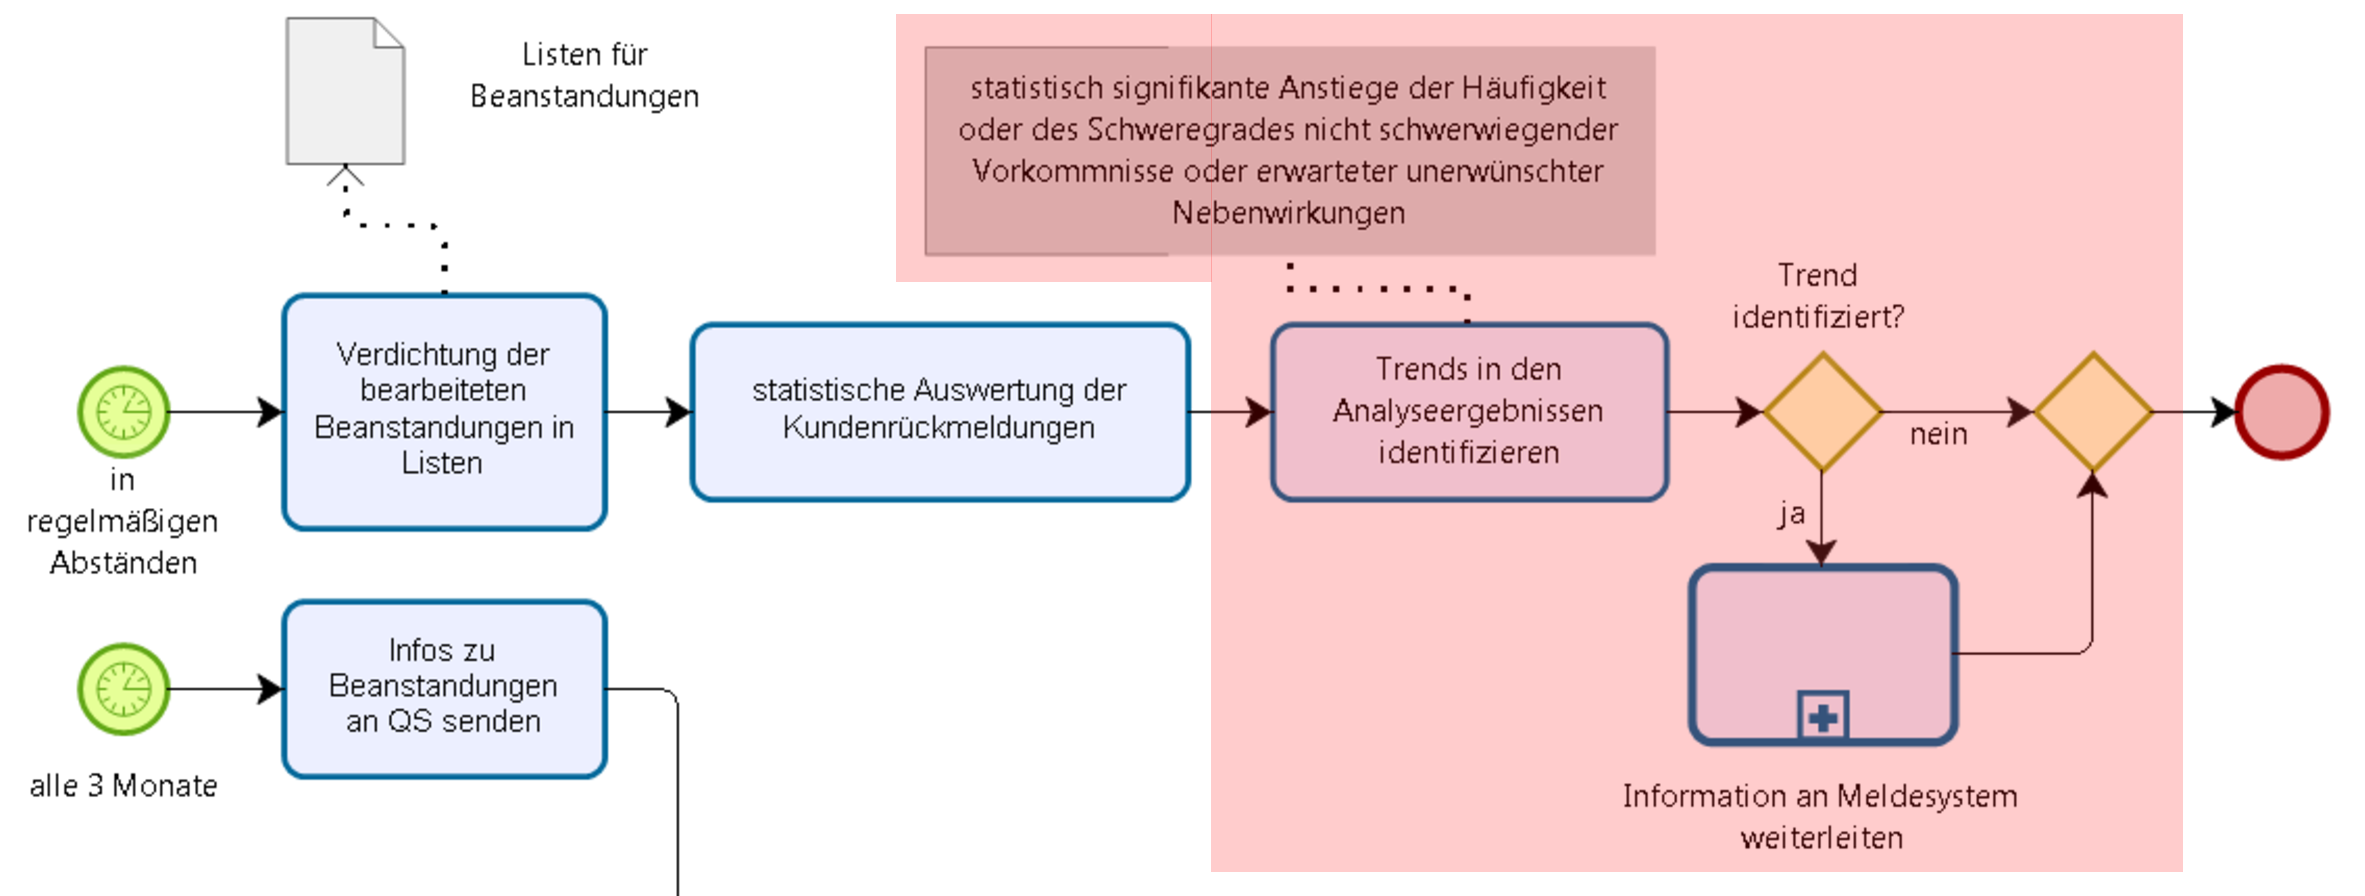
\includegraphics[width=1\textwidth]{Images/statistic_trend_analysis}
\caption[Erweiterung der statistischen Untersuchungen um Trendanalyse]{Erweiterung der statistischen Untersuchungen um Trendanalyse}
\label{statistic_trend_analysis}
\end{figure}
%===================================================================== Chapter 5
\chapter{Integration und Umsetzung der Prozessanpassungen}\label{chap:Integration}

%===================================================================== Zusammenfassung
\chapter{Zusammenfassung}\label{chap:Zusammenfassung}

%===================================================================== Diskussion
\chapter{Diskussion}\label{chap:Diskussion}

%===================================================================== Vorlagen
%\chapter{}\label{chap:}
%\section{}\label{sec:}
%\subsection{}\label{subsec:}
%\subsubsection{Requirements Engineering}  -- besitzt keine Nummerierung und taucht nicht im toc auf
%\cite[S. X]{<reference>}
%\ac{<Abkürzung>}

%===================================================================== Literaturverz.
\bibliography{literatur}
\bibliographystyle{alphadin}
%\bibliographystyle{abbrv}
% Übersicht unter: https://de.wikibooks.org/wiki/LaTeX-W%C3%B6rterbuch:_bibliographystyle

%===================================================================== Anhang
\appendix
\chapter[Anhang]{}
\newpage

% macros for checkboxes
\def\unchecked{\parbox[c]{1em}{
\includegraphics[width=1.15cm]{Images/checkbox_unchecked}}}
\def\checked{\parbox[c]{1em}{
\includegraphics[width=1.15cm]{Images/checkbox_checked}}}

\def\checkListTabHead{\begin{table}[!ht] \centering \begin{tabular}{|p{0.87\textwidth}|p{0.07\textwidth}|} \hline\vspace{0mm} Anforderung & \vspace{0mm}Erfüllt\\ \hline\hline}
\def\plainTabularTextWOCheckbox#1{\begin{tabular}{p{14,1cm}} \vspace{0mm}#1 \\\end{tabular} & \\}%{\vspace{0mm} #1 & \\}
\def\plainTabularTextChecked#1{\begin{tabular}{p{14,1cm}} \vspace{0mm}#1 \\\end{tabular} & \checked \\}
\def\plainTabularTextUnchecked#1{\vspace{0mm}#1 & \unchecked\\}
\def\tabularitemizeFirstLayerWOCheckbox#1{\begin{tabular}{p{0,3cm}p{13,4cm}}\vspace{0mm}\textbullet & \vspace{0mm}#1 \\\end{tabular} & \\}
\def\tabularitemizeFirstLayerCheck#1{\begin{tabular}{p{0,3cm}p{13,4cm}}\vspace{0mm}\textbullet & \vspace{0mm}#1 \\\end{tabular} & \checked\\}
\def\tabularitemizeFirstLayerUncheck#1{\begin{tabular}{p{0,3cm}p{13,4cm}}\vspace{0mm}\textbullet & \vspace{0mm}#1 \\\end{tabular} & \unchecked\\}
\def\tabularitemizeSecondLayerCheck#1{\begin{tabular}{p{0,3cm}p{0,3cm}p{12,7cm}}& - & #1 \\\end{tabular} & \checked\\}
\def\tabularitemizeSecondLayerUncheck#1{\begin{tabular}{p{0,3cm}p{0,3cm}p{12,7cm}}& - & #1 \\\end{tabular} & \unchecked\\}


\section{Checkliste für die Anforderungen der MDR}
\label{chap:ChecklistMDR}

\checkListTabHead
\plainTabularTextChecked{System zur Überwachung nach dem Inverkehrbringen (als integraler Bestandteil des QMS) muss eingerichtet sein, angewendet, instandgehalten und dauernd aktualisiert werden}
\hline
\plainTabularTextWOCheckbox{Plan zur Überwachung nach dem Inverkehrbringen:}
\tabularitemizeFirstLayerUncheck{Für die Überwachung nach dem Inverkehrbringen muss ein Plan erstellt werden, der Teil der technischen Dokumentation ist}
\tabularitemizeFirstLayerUncheck{Enthält u.A. Vorgehen, wie Trends erkannt werden (Methodik), zu behandeln sind und wie der Beobachtungszeitraum festgelegt wird}
\hline
\plainTabularTextChecked{Es werden Daten über Qualität, Leistung und Sicherheit eines Produktes während gesamter Lebensdauer gesammelt, aufgezeichnet, analysiert und verwendet für:}
\tabularitemizeFirstLayerCheck{Aktualisierung des Risikomanagements}
\tabularitemizeFirstLayerCheck{Aktualisierung der GA, Informationen zur Herstellung und Kennzeichnung}
\tabularitemizeFirstLayerCheck{Aktualisierung der klinischen Bewertung}
\tabularitemizeFirstLayerUncheck{Aktualisierung Kurzbericht über Sicherheit und klinische Leistung (für Klasse III Geräte)}
\tabularitemizeFirstLayerCheck{Ermittlung des Bedarfs an Präventiv-, Korrektur- oder Sicherheitskorrekturmaßnahmen im Feld}
\tabularitemizeFirstLayerCheck{Ermittlung von Möglichkeiten zur Verbesserung der Gebrauchstauglichkeit, der Leistung und der Sicherheit des Produkts}
\tabularitemizeFirstLayerUncheck{Gegebenenfalls Beitrag zur Überwachung anderer Produkte nach dem Inverkehrbringen}
\tabularitemizeFirstLayerCheck{Erkennung und Meldung von Trends}
\plainTabularTextChecked{Die Technische Dokumentation ist immer aktuell zu halten}
\hline
\ListTabBottom

\checkListTabHead
\plainTabularTextChecked{Durchführung und Überwachung von Präventiv- und Korrekturmaßnahmen aufgrund von gesammelten Daten inklusive Unterrichtung der zuständigen Behörden und gegebenenfalls benannter Stelle durch den Hersteller, bei schwerwiegenden Vorkommnissen und notwendigen Sicherheitskorrekturmaßnahmen im Feld}
\hline
\plainTabularTextWOCheckbox{Schwerwiegende Vorkommnisse oder Sicherheitskorrekturmaßnahmen im Feld:}
\tabularitemizeFirstLayerUncheck{Schwerwiegende Vorkommnisse, die im Zusammenhang zum Produkt stehen, werden den Behörden über elektronisches System gemeldet, außer es sind erwartete Nebenwirkungen laut Produktinformation, in technischer Dokumentation quantifiziert und durch Meldung von Trends erfasst}
\tabularitemizeSecondLayerUncheck{Meldung innerhalb 2 Tage nach Kenntnis der Gefahr, wenn schwerwiegende Gefahr für öffentliche Gesundheit besteht}
\tabularitemizeSecondLayerUncheck{Meldung innerhalb 10 Tage nach Kenntnis des Vorkommnisses, wenn Tod oder unvorhergesehener Verschlechterung des Gesundheitszustandes einer Person und Kausalzusammenhang zum Produkt besteht oder vermutet wird}
\tabularitemizeSecondLayerUncheck{Meldung innerhalb 15 Tage nach Kenntnis des Vorkommnisses, wenn Kausalzusammenhang zwischen Produkt und Vorkommniss festgestellt wurde oder möglich ist}
\tabularitemizeFirstLayerUncheck{Sicherheitskorrekturmaßnahmen im Feld, auch wenn Vorkommnis außerhalb der EU aufgetreten ist, aber Grund für Maßnahme direkt von einem Produkt, das auch in EU gehandelt wird, ausgeht, werden den zuständigen Behörden über elektronisches System gemeldet}
\tabularitemizeSecondLayerCheck{Meldung über Sicherheitskorrekturmaßnahme im Feld in nicht dringenden Fällen ohne gebührliche Verzögerung vor der Durchführung}
\tabularitemizeSecondLayerUncheck{Bei wiederholenden Meldungen (ähnliches Vorkommnis mit gleichem Produkt oder Produktart,  schon erfolgter Sicherheitskorrekturmaßnahme oder häufig auftretend aber gut dokumentiert) kann periodische Sammelmeldung über elektronisches System erfolgen}
\tabularitemizeFirstLayerCheck{Untersuchung  (u.A. Risikobewertung) folgt unverzüglich auf Meldung eines schwerwiegenden Vorkommnisses durch den Hersteller}
\tabularitemizeSecondLayerUncheck{Zusammenarbeit gegebenenfalls mit Behörden und benannter Stelle}
\tabularitemizeSecondLayerUncheck{Untersuchung muss sicherstellen, dass spätere Bewertung der Ursache des Vorkommnisses noch möglich ist oder Maßnahmen, die dagegen verstoßen würden, müssen vorher mit Behörde abgesprochen werden}
\tabularitemizeFirstLayerCheck{Notwendige Unterlagen müssen bei entsprechenden Anfragen an die Behörden ausgehändigt werden}
\hline
\ListTabBottom

\checkListTabHead
\tabularitemizeFirstLayerUncheck{Erstellung eines Abschlussberichtes (enthält Schlussfolgerungen und gegebenenfalls zu ergreifende Korrekturmaßnahmen) und Einreichung über elektronisches System}
\tabularitemizeFirstLayerUncheck{Bei ergriffenen Sicherheitskorrekturmaßnahmen im Feld müssen die Anwender mittels Sicherheitsanweisung im Feld über elektronisches System informiert werden}
\tabularitemizeSecondLayerUncheck{Entwurf der Anweisung wird koordinierender zuständiger Behörde vorgelegt (außer in dringenden Fällen), damit diese Anmerkungen abgeben kann}
\tabularitemizeSecondLayerUncheck{Identifikation über UDI und SRN}
\tabularitemizeSecondLayerUncheck{Enthalten sind Gründe für Sicherheitskorrekturmaßnahme im Feld mit Verweis auf Fehlfunktion und Risiken für Patienten, Anwender oder Dritte sowie alle zu ergreifenden Maßnahmen}
\tabularitemizeFirstLayerUncheck{Information über mögliche schwerwiegende Vorkommnisse können von zuständiger Behörde kommen, sofern diese zuerst informiert wurde}
\tabularitemizeSecondLayerUncheck{Behörde kann vom Hersteller Schritte gemäß schwerwiegendem Vorkommniss einfordern, auch wenn dieser ermittelt hat, dass Vorfall nicht schwerwiegend ist oder es als erwartete, unerwünschte Nebenwirkung, die in der Meldung von Trends enthalten sein wird, klassifiziert}
\hline
\plainTabularTextWOCheckbox{Bericht zur Überwachung nach dem Inverkehrbringen/Sicherheitsbericht:}
\tabularitemizeFirstLayerWOCheckbox{Klasse I:}
\tabularitemizeSecondLayerUncheck{Zur Zusammenfassung der Überwachung nach dem Inverkehrbringen und der ergriffenen Präventiv- und Korrekturmaßnahmen (Beschreibung und Begründung der Maßnahmen) muss ein Bericht erstellt werden}
\tabularitemizeFirstLayerWOCheckbox{Klasse IIa, IIb, III:}
\tabularitemizeSecondLayerUncheck{Ergebnisse und Schlussfolgerunge der PMS sowie Beschreibung und Begründung ergriffener Präventiv- und Korrekturmaßnahmen müssen enthalten sein (erstellt pro Produkt, gegebenenfalls Produktkategorie oder Produktgruppe)}
\tabularitemizeSecondLayerUncheck{Aktualisierung über gesamte Lebensdauer}
\tabularitemizeSecondLayerUncheck{Enthält:\newline a) die Schlussfolgerungen aus der Nutzen-Risiko-Abwägung\newline b) die wichtigsten Ergebnisse des Bewertungsberichts\newline c) die Gesamtabsatzmenge des Produkts und eine Schätzung der Anzahl und anderer Merkmale der Personen, bei denen das betreffende Produkt zur Anwendung kommt, sowie, sofern dies praktikabel ist, die Häufigkeit der Produktverwendung}
\hline
\ListTabBottom

\checkListTabHead
\tabularitemizeFirstLayerWOCheckbox{Aktualisierungsintervalle:}
\tabularitemizeSecondLayerUncheck{Klasse I: bei Bedarf und auf Anfrage der Behörden}
\tabularitemizeSecondLayerUncheck{Klasse IIa: mindestens alle 2 Jahre (Teil der technischen Dokumentation)}
\tabularitemizeSecondLayerUncheck{Klasse IIb: mindestens 1x jährlich (Teil der technischen Dokumentation)}
\tabularitemizeSecondLayerUncheck{Klasse III: mindestens 1x jährlich (Teil der technischen Dokumentation)}
\tabularitemizeFirstLayerWOCheckbox{Vorlage des Berichtes:}
\tabularitemizeSecondLayerUncheck{Klasse I: bei benannter Stelle oder auf Anfrage durch Behörde}
\tabularitemizeSecondLayerUncheck{Klasse IIa, IIb, Sonderanfertigungen: über elektronisches System bei benannter Stelle oder auf Anfrage durch Behörde}
\tabularitemizeSecondLayerUncheck{Klasse III und implantierbare Produkte: über elektronisches System an benannte Stelle}
\tabularitemizeFirstLayerUncheck{Bei Sonderanfertigungen separate Struktur der Dokumentation}
\hline
\plainTabularTextWOCheckbox{Trends:}
\tabularitemizeFirstLayerUncheck{Meldung von statistisch signifikanten (entscheidend ist Vergleich mit erwartetem und in techn. Doku angegebener Häufung) Anstiegen der Häufigkeit oder des Schweregrades nicht schwerwiegender Vorkommnisse oder erwarteter unerwünschter Nebenwirkungen über elektronisches System, wenn Nutzen-Risiko-Analyse erheblich beeinflusst wird und Risiken für die Gesundheit entstehen}
\tabularitemizeFirstLayerUncheck{Behörden können bei abweichender Einschätzung  der Meldung vom Hersteller verlangen, Maßnahmen zu ergreifen}
\hline
\plainTabularTextWOCheckbox{Klinische Nachbeobachtung nach dem Inverkehrbringen
(PMCF):}
\tabularitemizeFirstLayerCheck{Ist Teil des Qualitätsmanagementsystems und wird aufgestellt, angewendet, aufrechterhalten und auf dem neuesten Stand gehalten}
\tabularitemizeFirstLayerUncheck{Prozess der klinischen Nachbeobachtung nach dem Inverkehrbringen aktualisiert klinische Bewertung während gesamter Lebensdauer und ist Teil des Plans zur Überwachung nach dem Inverkehrbringen}
\hline
\ListTabBottom

\checkListTabHead
\tabularitemizeFirstLayerCheck{Klinische Daten, die bei zweckgemäßer Verwendung erhoben werden, werden proaktiv gesammelt und ausgewertet, um:}
\tabularitemizeSecondLayerCheck{Sicherheit und Leistung während der Lebensdauer zu bestätigen}
\tabularitemizeSecondLayerCheck{Konformität der ermittelten Risiken sicherzustellen}
\tabularitemizeSecondLayerCheck{Neu entstehende Risiken und Nebenwirkungen auf Grundlage empirischer Belege zu identifizieren}
\tabularitemizeSecondLayerCheck{Vertretbarkeit Nutzen-Risiko-Verhältnis zu gewährleisten}
\tabularitemizeSecondLayerCheck{Systematisch fehlerhafte oder zulassungsüberschreitende Verwendung festzustellen (Prüfung auf Angemessenheit der Zweckbestimmung)}
\tabularitemizeFirstLayerUncheck{Ein Plan wird erstellt, der folgendes enthält:}
\tabularitemizeSecondLayerUncheck{Allgemein anzuwendende Methoden und Verfahren zur Erhebung und Begründung der Eignung}
\tabularitemizeSecondLayerUncheck{Verweis auf relevante Teile des Berichts über klinische Bewertung und das  Risikomanagement}
\tabularitemizeSecondLayerUncheck{Abzudeckende spezifische Ziele}
\tabularitemizeSecondLayerUncheck{Bewertung der klinischen Daten zu gleichartigen oder ähnlichen Produkten}
\tabularitemizeSecondLayerUncheck{Verweis auf GS (gemeinsame Spezifikation), harmonisierte Normen (wenn angewendet) und einschlägige Leitlinien zum Thema}
\tabularitemizeSecondLayerUncheck{Zeitplan für die geplanten Tätigkeiten}
\tabularitemizeFirstLayerCheck{Ergebnisse werden in Bewertungsbericht, der Teil der technischen Dokumentation ist, dokumentiert}
\tabularitemizeFirstLayerUncheck{Schlussfolgerungen werden bei klinischer Bewertung und Risikomanagement berücksichtigt}
\tabularitemizeFirstLayerUncheck{Notwendigkeit zur Durchführung von Präventiv-/ oder Korrekturmaßnahmen im Feld wird ermittelt und Prozesse entsprechend gestartet}
\tabularitemizeFirstLayerUncheck{Durchführung von Studien über klinische Nachbeobachtung nach dem Inverkehrbringen, die von benannten Stelle gefordert werden}
\hline
\ListTabBottom

\checkListTabHead
\plainTabularTextWOCheckbox{Analyseaktivitäten der Behörden:}
\tabularitemizeFirstLayerUncheck{Unterlagen und Informationen für Behörden zwecks Durchführung der Marktüberwachung zur Verfügung stellen}
\tabularitemizeFirstLayerUncheck{Produktstichproben oder Zugang zu Produkten bei gerechfertigtem Anliegen den Behörden kostenfrei zur Verfügung stellen}
\tabularitemizeFirstLayerUncheck{Hersteller ergreift erforderliche Korrekturmaßnahmen, wenn Behörden aus der Analyse der Vigilanz-Daten Risiken oder nachteilige Änderugen der Nutzen-Risiko-Abwägung ermitteln und dem Hersteller mitteilen}
\tabularitemizeFirstLayerUncheck{Kooperation bei Bewertung eines Produktes aufgrund des Verdachtes}
\tabularitemizeSecondLayerUncheck{Eines unvertretbaren Risikos für die Gesundheit oder Sicherheit oder für Aspekt des Schutzes der öffentlichen Gesundheit}
\tabularitemizeSecondLayerUncheck{Anderweitig nicht erfüllte Anforderungen der Verordnung}
\tabularitemizeFirstLayerUncheck{Prüfung des durch die Behörde erstellten Berichtes über eine durchgeführte Kontrolle und gegebenenfalls Verfassung einer Stellungnahme durch den Hersteller, die in elektronischem System in Form einer Stellungnahme erfasst wird}
\tabularitemizeFirstLayerUncheck{Zuständige Behörde kann zu Ergreifung von geeigneten und gebührend gerechtfertigten Korrekturmaßnahmen bei vertretbaren und unvertretbaren Risiken  für die Gesundheit oder Sicherheit der Patienten, Anwenders oder anderer Personen oder in Bezug auf andere Aspekte des Schutzes der öffentlichen Gesundheit auffordern, um Konformität des Produkts herzustellen (Bereitstellung des Produktes, die der Art des Risikos angemessen ist, Beschränkung des Risikos, Bereitstellung des Produktes bestimmten Anforderungen unterwerfen, Produkt vom Markt nehmen, Produkt zurückrufen)}
\tabularitemizeSecondLayerUncheck{Notwendige Korrekturmaßnahme in gesamter europäischer Union durchführen, wo betroffenes Produkt auf dem Markt verfügbar ist}
\tabularitemizeFirstLayerUncheck{Unterstützung der Kommission, bei der Überprüfung der Rechtmäßigkeit von getroffenen Maßnahmen eines Mitgliedsstaates, wenn Einwände eines anderen Mitgliedsstaates dagegen bestehen oder Kommission die Maßnahme für nicht mit dem Unionsrecht vertretbar einschätzt, in Form von Anhörungen}
\tabularitemizeFirstLayerUncheck{Unterstützung der Kommission in Form von Absprache zur Prüfung getroffener Maßnahmen nationaler Behörden, wenn erforderlich}
\hline
\ListTabBottom
%===================================================================== Eidessattl. Vers.
\chapter*{Eidesstattliche Versicherung} %  *-> erstellt unnummeriertes chapter
Ich versichere, dass ich die vorliegende Arbeit selbstständig verfasst, keine anderen als die angegebenen Quellen und Hilfsmittel benutzt sowie alle wörtlich oder sinngemäß übernommenen Stellen in der Arbeit gekennzeichnet habe.
\\[2cm]
\noindent\rule{0.35\textwidth}{0.3pt}\rule{0.2\textwidth}{0pt}\rule{0.45\textwidth}{0.3pt}
\\Ort, Datum\rule{0.418\textwidth}{0pt}Unterschrift
\end{document}